%------------------------------------------------------------------------------%
%%%%%%%%%%%%%%%%%%%%%%%%%%%%%  DISE�O  %%%%%%%%%%%%%%%%%%%%%%%%%%%%%%%%%%%%%%%%%
%------------------------------------------------------------------------------%

\NeedsTeXFormat{LaTeX2e}
\documentclass[12pt]{book}

\usepackage{a4}
\usepackage[Lenny]{fncychap}    % Estilos para capitulos
\usepackage{fancyhdr}           % Estilos para cabeceras
\usepackage[english]{babel}
\usepackage[latin1]{inputenc}
\usepackage{epsfig}
\usepackage{subfig}
\usepackage[font={small,it}]{caption}
\usepackage{keyval}
\usepackage{graphicx}
\usepackage{float}              % Para poner las imags en cualquier sitio
\usepackage{lettrine}						% Para poner la primera letra de cada cap�tulo y/o p�rrafo en grande.
\usepackage{color}

\usepackage[usenames,dvipsnames,svgnames,table]{xcolor}

\usepackage[numbers,sort&compress,comma]{natbib}	% Modo de poner la bibliograf�a
\usepackage{verbatim}      %  \begin{comment}...\end{comment}
\usepackage{subeqnarray}   % equationarray with numbers 1a, 1b, ...
\usepackage{bbm}           % Para s�mbolo tipo n�meros reales. Ej: \bbm{R}
\usepackage{longtable}     % Para tablas largas de m�s de una p�gina
\usepackage{psfrag}        % Para cambiar fragmentos de text en .eps por otro en latex
\usepackage{pifont}        % Para otros s�mbolos
\usepackage{fancybox}      % Para encuadrar texto en recuadros
\usepackage{amsmath}       % Mejora la calidad de las formulas
%\usepackage{amsfonts}
\usepackage{kpfonts}
\usepackage[hyphens]{url}
\usepackage[linktocpage]{hyperref}      % Para enlaces de hipertexto
\usepackage{amssymb}
\usepackage{multirow}
\usepackage{booktabs}
\usepackage{listings}
\usepackage{fancyvrb}
\usepackage{enumerate}
\usepackage{wrapfig}
\usepackage{eurosym}
\usepackage{multicol}
\usepackage{pifont}
\usepackage{epstopdf}
\usepackage{mathtools}


\setcounter{tocdepth}{3}             % toc = table of contents. Para definir niveles del �ndice
\setcounter{secnumdepth}{3}          % Hasta cu�ndo se enumeran los caps, seccs, etc
\setlength{\topmargin}{-1.1cm}        % margen por arriba
\setlength{\parskip}{0.3cm}          % Espacio entre parrafos
\setlength{\textwidth}{15.5cm}       % Ancho del �rea imprimible	
\setlength{\evensidemargin}{-0.1cm}  % Margen izdo en p�ginas pares
\setlength{\oddsidemargin}{0.6cm}    % Margen izdo en p�ginas impares
                                     % evensidemargin = -oddsidemargin !!!

\setlength{\headsep}{1.0cm}
\setlength{\headheight}{3ex}
\setlength{\footnotesep}{5mm}

\renewcommand{\LettrineFontHook}{\color[gray]{0.5}} % Pone la letrina en gris.



%\setlength{\mathindent}{1.0cm}       % Controla el espacio entre margen y ec si no est� centrada

%%% Definitionen f�r Fancy Headings
%\renewcommand{\baselinestretch}{3mm}
%\renewcommand{\labelenumi}{\roman{enumi}.}
%\renewcommand{\chaptermark}[1]{\markboth{#1}{}}
%\renewcommand{\sectionmark}[1]{\markright{\thesection\ #1}{}}


%\renewcommand{\listtablename}{�ndice de tablas}
%\renewcommand{\tablename}{Tabla}


\lhead[\fancyplain{}{\thepage}]{\fancyplain{}{\sl\nouppercase\rightmark}}
\rhead[\fancyplain{}{\sl\nouppercase\leftmark}]{\fancyplain{}{\thepage}}
\cfoot{}
\pagestyle{fancyplain}  		% normale Kopfzeile; ohne Seitenzahl: empty

% Formato de capitulos
\ChTitleVar{\sf\Huge} % Tama�o de la letra del nombre del cap
\ChTitleAsIs


%%% Comando para quitar encabezado y pie de las pag en blanco
\newcommand{\clearemptydoublepage}
  {\newpage{\pagestyle{empty}\cleardoublepage}}

\newcommand{\R}{\mathbb{R}}
\newcommand{\x}{\mathbf{x}}

%%% Abstract
\newenvironment{abstract}
  {\begin{center}
   \begin{minipage}{0.8\textwidth}
   \slshape}
  {\end{minipage}
   \end{center}}


\typeout{ }
\typeout{----------------------------------------------------------------------}
\typeout{ }


%------------------------------------------------------------------------------%
%%%%%%%%%%%%%%%%%%%%%%%%%%%%%%  DOCUMENTO  %%%%%%%%%%%%%%%%%%%%%%%%%%%%%%%%%%%%%
%------------------------------------------------------------------------------%

\begin{document}

  \begin{titlepage}
\label{ch:cover}
\begin{center}

{\Large\textsc{Telecomunication Engeneering}}


Department:  \\ Signal Theory, Telematics and Communications

\textbf{University of Granada}


\vspace{0.5cm}

\begin{figure}[h]
	\centering
	
\epsfig{file=imagenes/ugr, width=7cm}
	\label{fig:ugr}
\end{figure}


\vspace{0.5cm}
\textbf{Master thesis}


\vspace{0.9cm}


{\Huge\textbf{Comparison of Posturographic Body-sway Measurements with Inertial Data of Parkinson Patients }}


\end{center}


\vspace{1.5cm}
\textbf{Written by:}  \hfill \textbf{Supervised by:}

Ver\'onica Torres S\'anchez \hfill    D. Juan Manuel Górriz Sáez(UGR)

							\hfill	  D. Javier Ramírez Pérez de Inestrosa (UGR)
							
							\hfill    D. Alberto Olivares Vicente (UMU)
							
							\hfill	  D. Kai Bötzel (UMU)


\end{titlepage}
						% Inclu�mos la portada en espa�ol
  \clearemptydoublepage	
	
  \pagenumbering{arabic}     % Numeraci�n de p�ginas con num romanos
  %\setcounter{page}{1}      % Establece la siguiente p�gina como la 1
  \addtocontents{toc}{\protect\sloppy}
  %\clearemptydoublepage
  \tableofcontents          % Pone �ndice
  %\pagenumbering{arabic}    % Numeraci�n de p�ginas con num normales (�rabes)
  %\setcounter{page}{1}      % Establece la siguiente p�gina como la 1
  \addtocontents{lof}{\protect\sloppy}
  \clearpage
  \listoffigures						% Crea la lista de figuras
	\addtocontents{lot}{\protect\sloppy}
  \clearemptydoublepage
	\listoftables							% Crea la lista de tablas
  \clearemptydoublepage
  %%% Capitulos
	\clearemptydoublepage
  \chapter{The GaitWatch Device}
\label{ch:gaitwatch}

\section{General description}
\indent GaitWatch is an Inertial Measurement Unit (IMU) designed for gait monitoring purposes. It was developed by Prof. Dr. Med. Kai B\"otzel at the Department of Neu\-ro\-lo\-gy of Ludwig-Maximilians University in Munich in conjunction with Dr. Alberto Olivares Vicente from the Department of Signal Theory, Telematics and Communications of the University of Granada. \\
GaitWatch is thought to be used in applications in which it is necessary to monitor the motion of patients. \\
\indent The system is composed of a box which contains the central processing unit and a set of measuring units which are wired to it. The measuring units are thought to be placed in the patients' thighs, shanks, arms and trunk. Figure XXXX shows the appearance of the complete GaitWatch device. 

\section{Hardware description}
\indent As it was aforementioned, GaitWatch has a box containing the central processing unit as well as a set of embedded magnetic and inertial sensors. The microcontroller acting as the central processing unit is in charge of gathering the data from the external measurement units and writing it to the memory card together with the data from the embedded box sensors. \\

\indent There are two different kinds of external units. The first one (type A IMU) is placed on both thighs and shanks. The second unit (type B IMU) is placed on both arms. Figure \ref{fig:GWdiagram} shows a diagram of the box (which contains the CPU and the type C IMU) together with the external units. 

\begin{figure}[H]
\centering
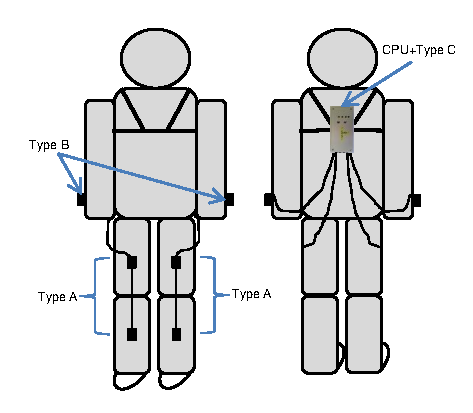
\includegraphics[width=0.8\textwidth]{figures/GWdiagram}
\caption{General diagram of the GaitWatch being worn by a subject.}
\label{fig:GWdiagram}
\end{figure}

\indent The three different kinds of IMUs have the following components:

\begin{itemize}
	\item Type A (thighs and shanks): 
	\begin{itemize}
		\item IMU 5 \cite{imu5} from Sparkfun. IMU 5 contains an IDG500 \cite{idg500} biaxial gyroscope (from which only Y axis is actually used) with a measurement range of $\pm500deg/s$ and a $\pm3g$ triaxial accelerometer, ADXL335 \cite{adxl335}.
	\end{itemize}
	\item Type B (arms):
	\begin{itemize}
		\item IDG500 \cite{idg500} biaxial $\pm500deg/s$ gyroscope.
	\end{itemize}
	\item Type C (trunk box):
	\begin{itemize}
		\item ADXL345 \cite{adxl345} triaxial accelerometer with programmable range ($\pm16g/\pm8g/\pm4g/\pm2g$).
		\item IMU3000 \cite{imu3000}triaxial gyroscope with programmable range ($\pm250/\pm500/\pm1000/\pm3000 (deg/s)$).
		\item Micromag3 \cite{micromag3} triaxial magnetometer ($\pm11Gauss$).
	\end{itemize}
\end{itemize}

In addition, the trunk box contains an AL-XAVRB \cite{avratx} board containing an AVR ATxmega processor which contains the necessary embedded firmware to gather the data from all the measurement units and store it in a microSD card.

Figure XXX shows the schematics of the complete GaitWatch device.


  \clearemptydoublepage
  \chapter{Initial configuration}
\label{ch:initial_conf}
\section{Identification of sensor's axes}
\indent The first step that needs to be carried out is to determine the orientation of the axes of the body frame that we wish to use, as well as the orientation of the rotation around those axes. One of the most popular configurations is to set the X axis pointing forwards, the Y axis pointing to the right and the Z axis pointing down. This configuration follows the rule of the right hand for the orientation of the axes and the corkscrew rule for the rotation. Both are shown in Figure \ref{fig:bodyAxes}. These two standard navigation frames are usually employed when representing the orientation of a body in space and are known as the North-East-Down (NED) and the East-North-Up (ENU) frames.

\begin{figure}[H]
\centering
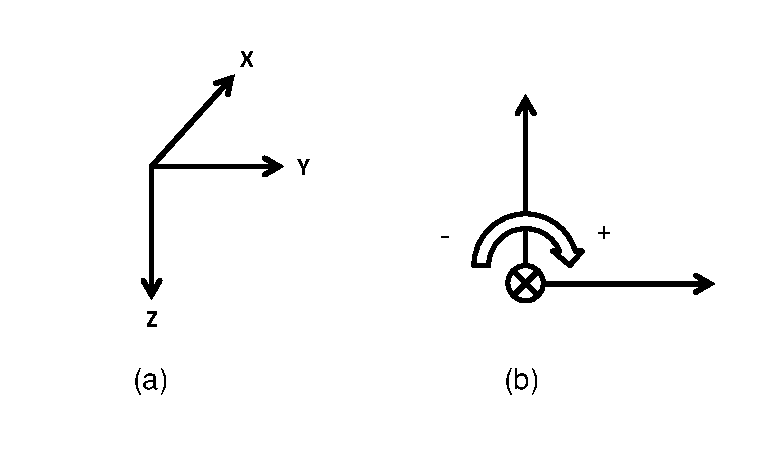
\includegraphics[width=0.6\textwidth]{figures/bodyAxes}
\caption{Definition of the desired body axes (a). Convention for the orientation of the axis rotation (b).}
\label{fig:bodyAxes}
\end{figure}
Since we will be using the GaitWatch device to monitor gait, then we need its X axis to point to the front of the patient, the Y axis pointing to the right of the patient, and the Z axis to the floor. We will start by configuring the orientation of the sensors which are inside the data gathering unit and which will be placed on the back of the patient. Figure \ref{fig:gwBox} shows the desired orientation for Gaitwatch's box.

\begin{figure}[H]
\centering
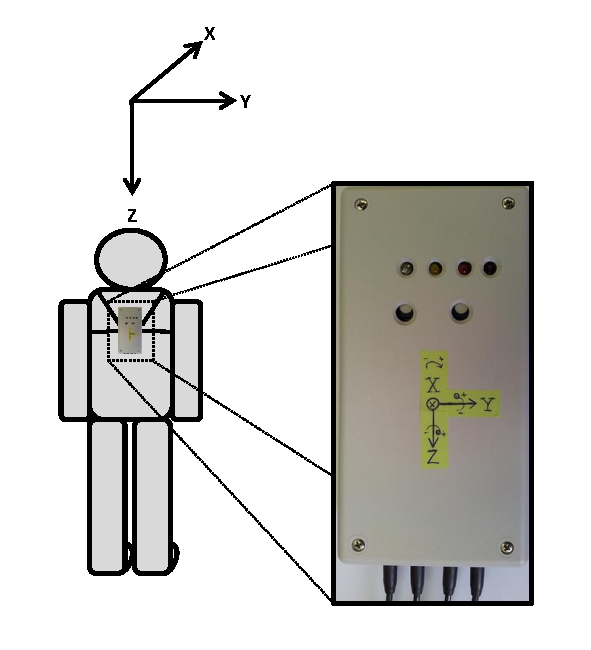
\includegraphics[width=0.6\textwidth]{figures/bodyAxesGW}
\caption{Orientation and axes of the GaitWatch box.}
\label{fig:gwBox}
\end{figure}

Once we know the desired orientation, the next step is to adapt the axes of the sensors' boards to it. We will start by adjusting the accelerometer. 

\subsection{Identification of Accelerometer's axes}
\label{subsec:acc_ID}

\indent The goal here is to determine the orientation of the axes and adapt it to the convention aforementioned. First, we set the box with the desired Z axis pointing downwards and upwards respectively while gathering data, as shown in figure \ref{fig:AccZaxis}.

Now we plot the acceleration gathered along the three axes. We have to identify the channel showing a large change in the measured acceleration.

\begin{figure}[H]
\centering
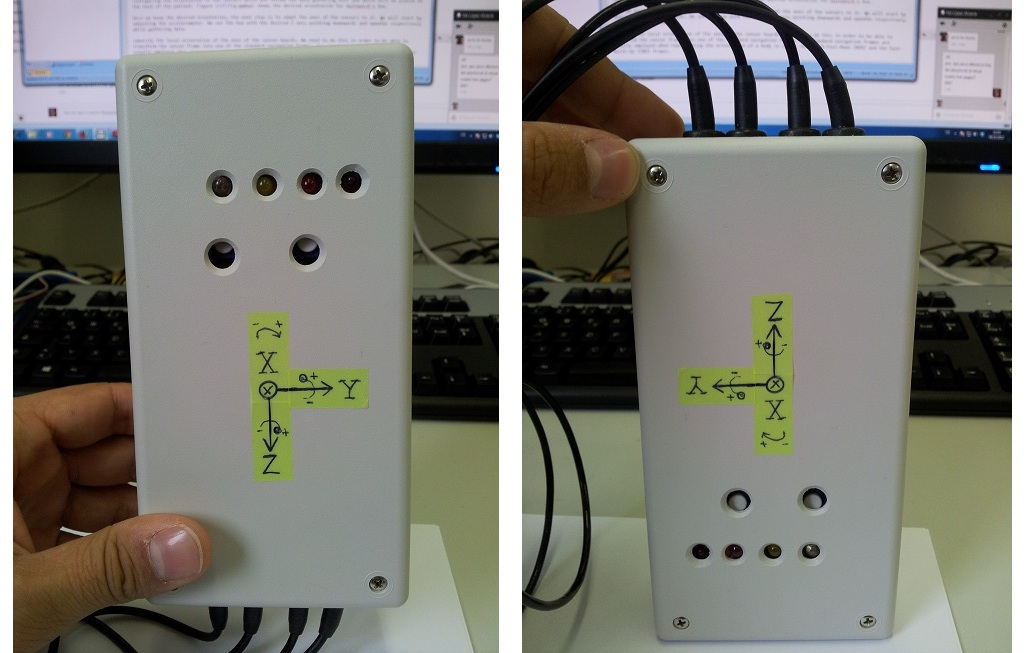
\includegraphics[width=0.6\textwidth]{figures/AccZaxis.jpg}
\caption{Identification of Z axis of the accelerometer in the box unit.}
\label{fig:AccZaxis}
\end{figure}
 
That channel will then be labeled as Z irrespective to which label it may have in the accelerometer board. That is, the sensor board may indicate that the selected channel is 'X' in the sensor frame, but we will label it as 'Z' in our desired frame which is the body frame. 

If the Z axis of the sensors has the same orientation of the desired frame, then, when pointing the Z axis of the box downwards, the accelerometer will measure 1g since its axis is parallel to the Earth's gravity vector. If it has the opposite orientation, then the accelerometer will measure -1g. Since we have not calibrated the accelerometer so far and, therefore, the data are in raw units, the way to identify the correct orientation is by knowing that the measured output when setting the accelerometer axis parallel to gravity is larger than its output when it is set anti-parallel to the gravity vector. Figure \ref{fig:ZaxisAccSignals} shows the triaxial gathered acceleration and the axis which should be labeled as 'Z'.

\begin{figure}[H]
\centering
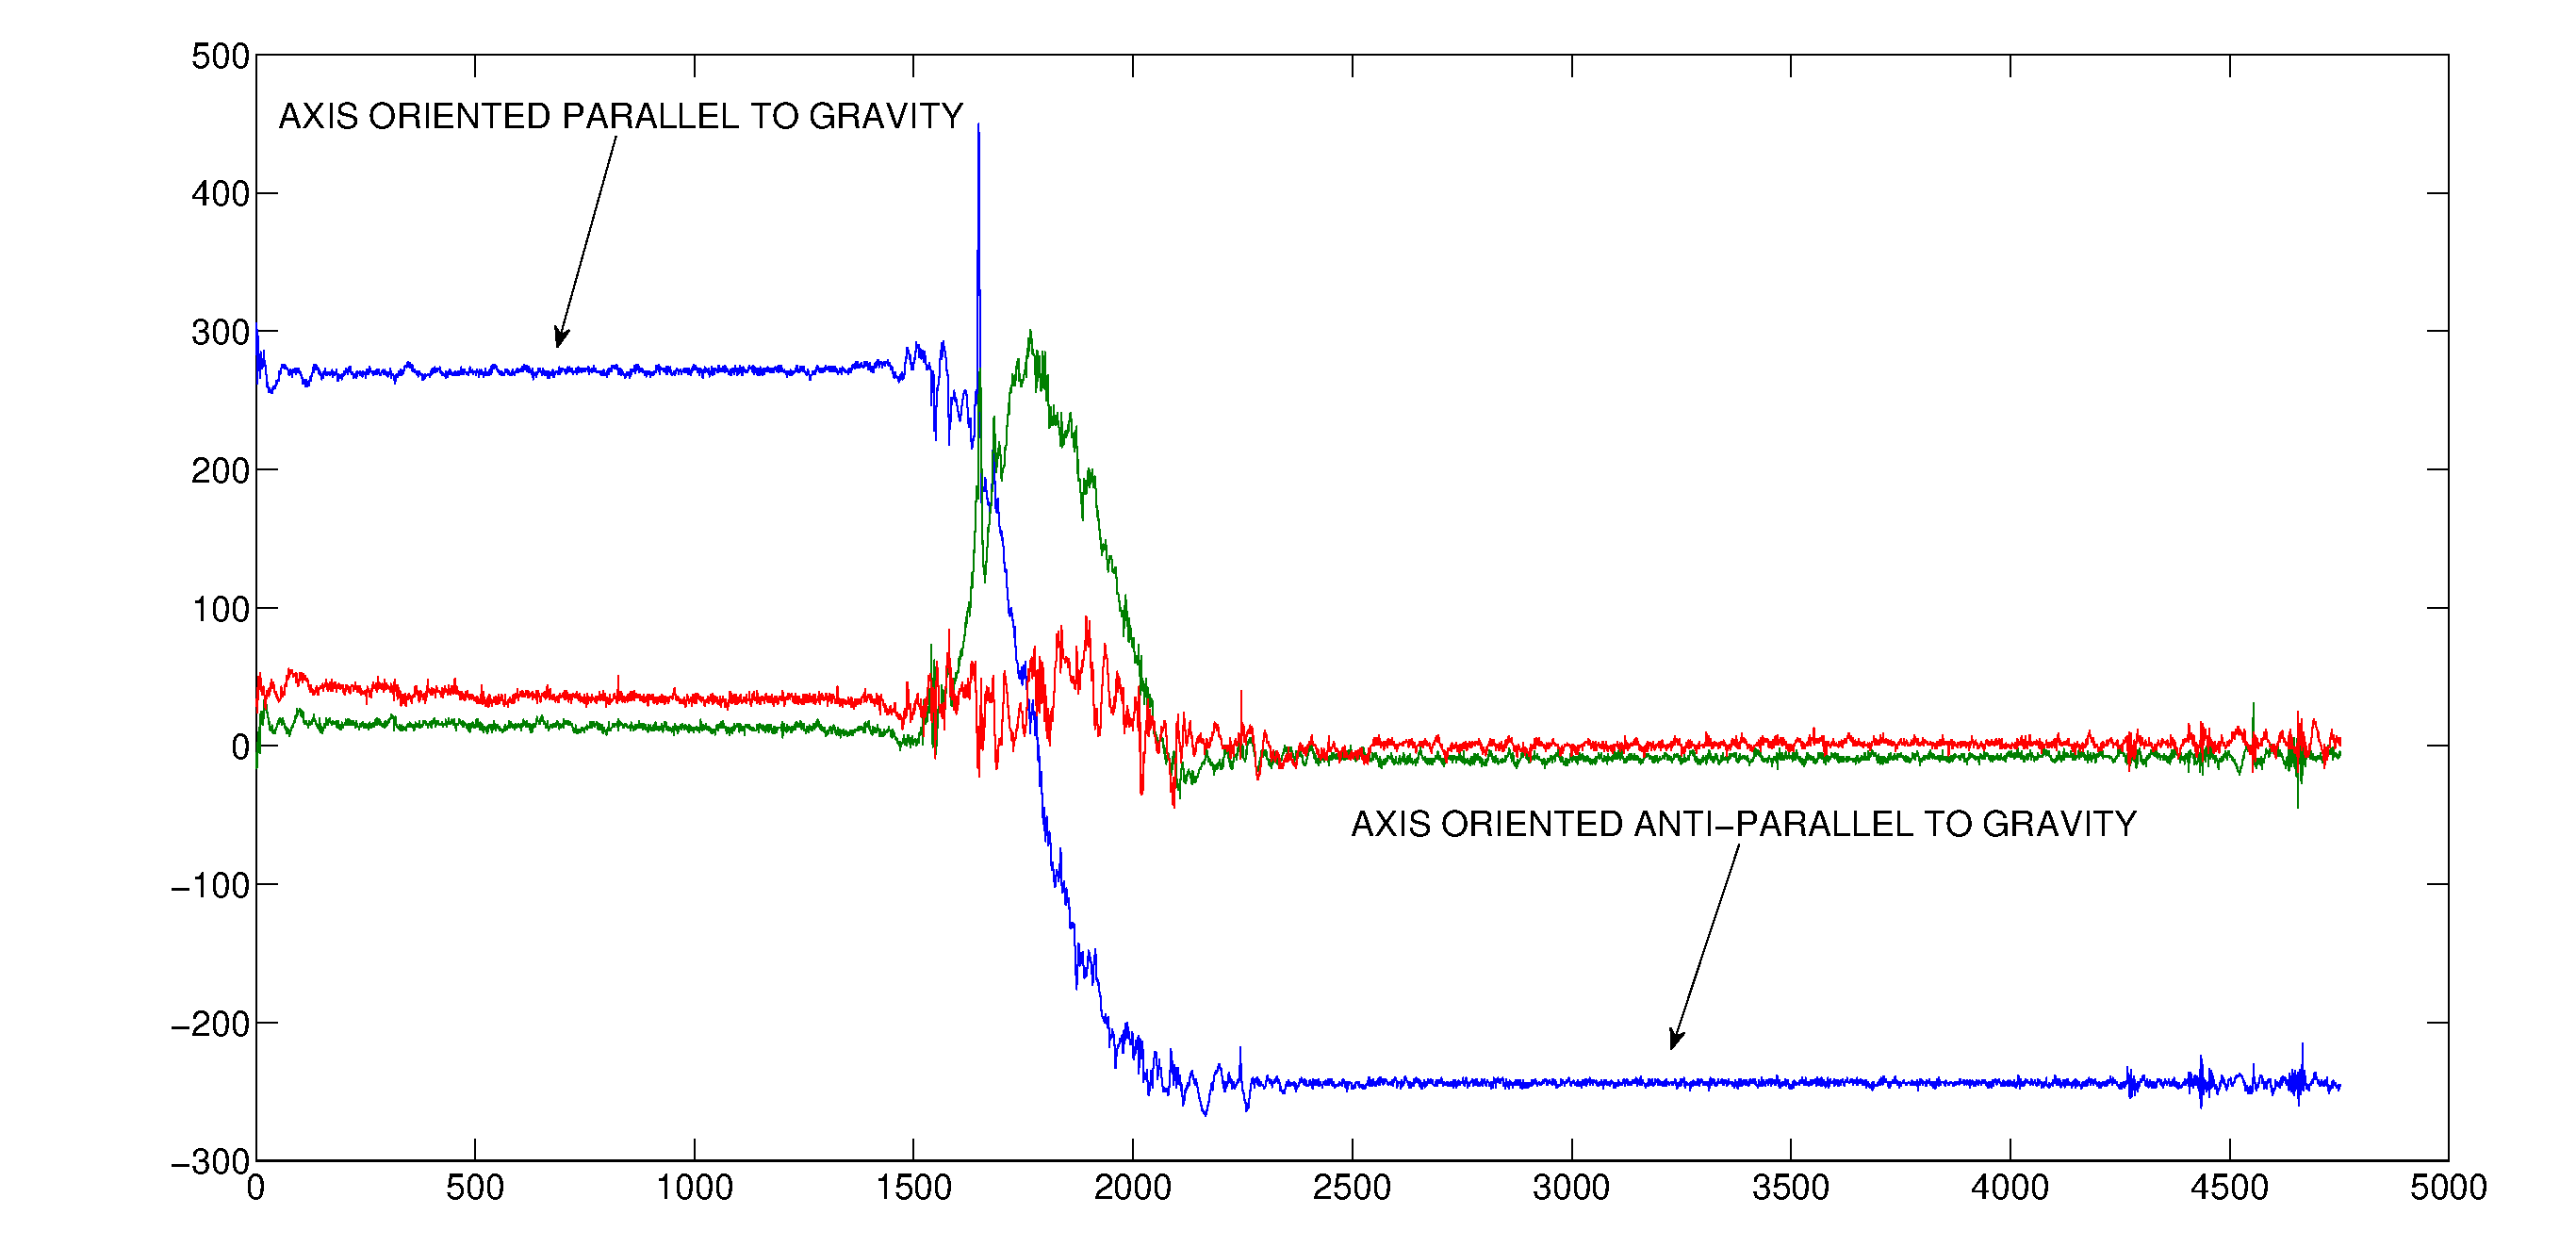
\includegraphics[width=0.85\textwidth]{figures/ZaxisAccTrunkID}
\caption{Identification of the acceleration signal gathered in the Z axis.}
\label{fig:ZaxisAccSignals}
\end{figure}

For the case of the GaitWatch, the signal showing both parallel and anti-parallel acceleration values is in channel 20. The orientation of the axis is correct, since we first put the desired Z axis pointing downwards and the accelerometer showed the largest acceleration value in that position. We, thus, set channel 20 to be the acceleration in Z axis. The remaining two axes (X and Y) are identified following the same procedure. Figure \ref{fig:XandYAccPositions} shows the box being oriented negatively and positively along X and Y axes. Both X and Y axes are properly oriented and need no orientation correction. After inspecting the gathered signals, we observe that X and Y measurements are contained in channels 22 and 21, respectively. 

\begin{figure}[H]
\centering
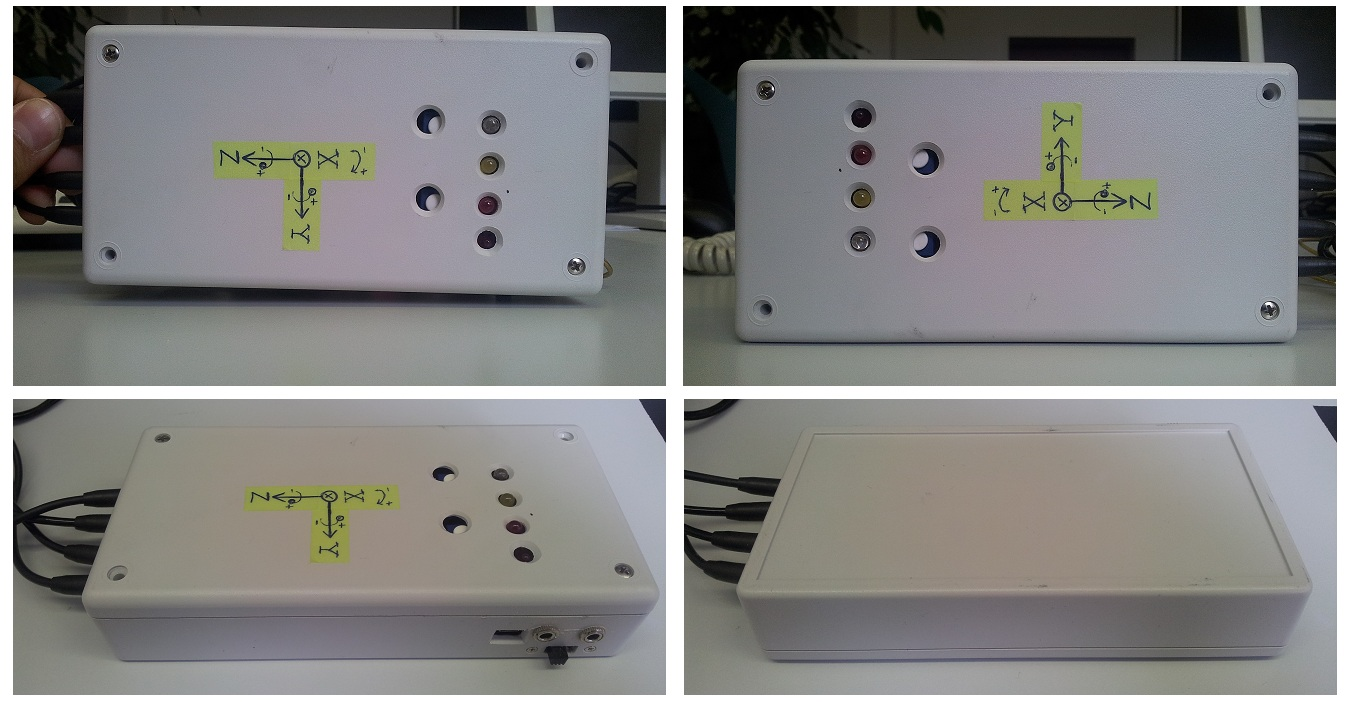
\includegraphics[width=0.7\textwidth]{figures/XandYAccPositions.jpg}
\caption{Identification of the box's acceleration Y (top) and X (bottom) axes.}
\label{fig:XandYAccPositions}
\end{figure}

Once we have identified the axes of the accelerometer inside the box which will be placed in the back of the patient, we need to apply the same aforementioned procedure to identify, on by one, the axes of the biaxial accelerometers which will be placed in the thighs and the shanks. Figure \ref{fig:thighShankAccs} shows the right shank module being placed parallel and anti-parallel to the gravity in both X and Z axes.

\begin{figure}[H]
\centering
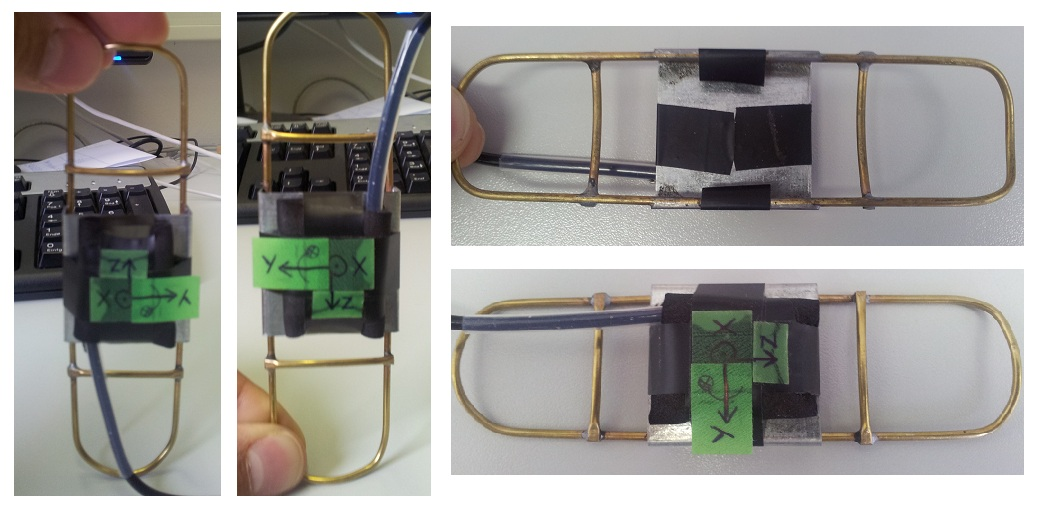
\includegraphics[width=0.7\textwidth]{figures/thighShankAccs.jpg}
\caption{Identification of the Z (left) and X (right) axes of the accelerometer in right shank's unit.}
\label{fig:thighShankAccs}
\end{figure}

Table \ref{tab:acc_channels} shows the axes of all Gaitwatch's accelerometers, their associated channel and the orientation compensation (if needed).
\begin{table}
\caption{List of Gaitwatch's accelerometers and their associated channels.}
	\centering
		\begin{tabular}{|c|c|c|c|}\hline
		\label{tab:acc_channels}
		Unit 				& Axis 	& Orientation compensation 	& Channel 	\\ \hline
		Right Shank & Z			& No  (+1)									& 2					\\
		Right Shank	& X			& No  (+1)									& 3					\\
		Right Thigh & Z			& No  (+1)									& 5					\\
		Right Thigh	& X			& No  (+1)									& 6					\\
		Left Shank  & Z			& No  (+1)									& 8					\\
		Left Shank	& X			& No  (+1)									& 9					\\
		Left Thigh  & Z			& No  (+1)									& 11				\\
		Left Thigh	& X			& No  (+1)									& 12				\\
		Trunk				& Z			& No	(+1)									& 20				\\
		Trunk				& Y			& No	(+1)									& 21				\\	
		Trunk				& X			& No	(+1)									& 22				\\ \hline
		\end{tabular}
\end{table}

\subsection{Identification of Gyroscope's axes}
\label{subsec:gyro_ID}

\indent Once we have identified the axes of the accelerometers, we now proceed to identify the axes of the gyroscopes and their orientation. By convention, as it is depicted in figure \ref{fig:bodyAxes}, the sense of the rotation around a given axis is positive when the axis is pointing forwards (from the perspective of the user) and it is turned to the right. Analogously, the rotation is negative when it is turned to the left. Knowing this, in order to identify the sense of rotation of the gyroscope and adapt it (if needed) to the body frame we need to proceed as follows:
\begin{enumerate}
\item Place the axis that we want to analyze so it is pointing forwards.
\item Rotate it to the right and then to the left. Repeat this three of four times. 
\item Identify the channel containing the data and plot them. If the measured angular rate first increases and then decreases, the sense of rotation of the sensor axis is correct. On the other hand, if the angular has the opposite behavior, that is, it first decreases and then increases, we need to change the sense of the rotation. 
\end{enumerate}
Figure \ref{fig:rotation_axis_sense1} shows the maneuvers to identify the rotation sense of the Y axis gyroscope located in the left hand unit. Figure \ref{fig:rotation_axis_sense2} shows the measured angular rate for such maneuvers. Notice how the first rotation is positive (the signal increases and then decreases), so, for the case of the left hand unit, the Y axis has the correct sense of rotation.

\begin{figure}[H]
\centering
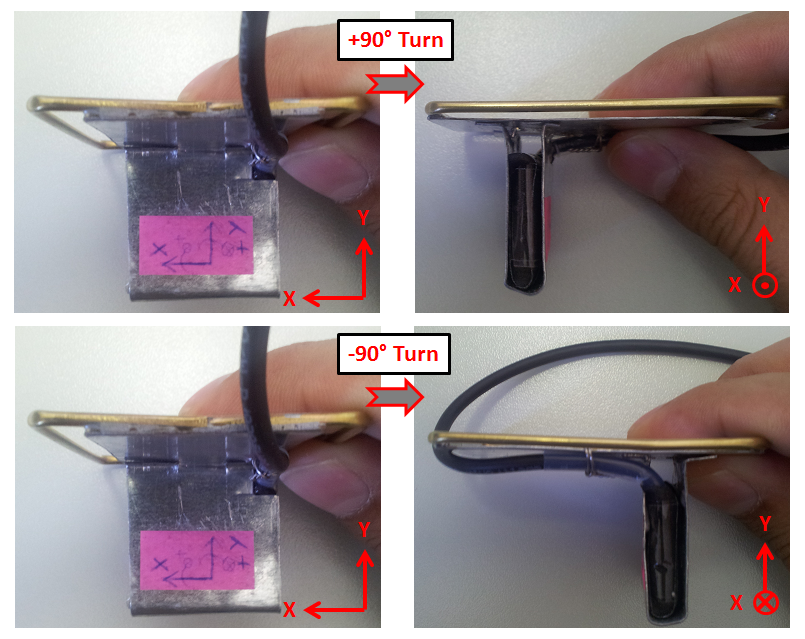
\includegraphics[width=0.7\textwidth]{figures/gyro_axis_ID.png}
\caption{Identification of the sense of rotation of the Y axis of the gyroscope in the left hand unit.}
\label{fig:rotation_axis_sense1}
\end{figure}

\begin{figure}[H]
\centering
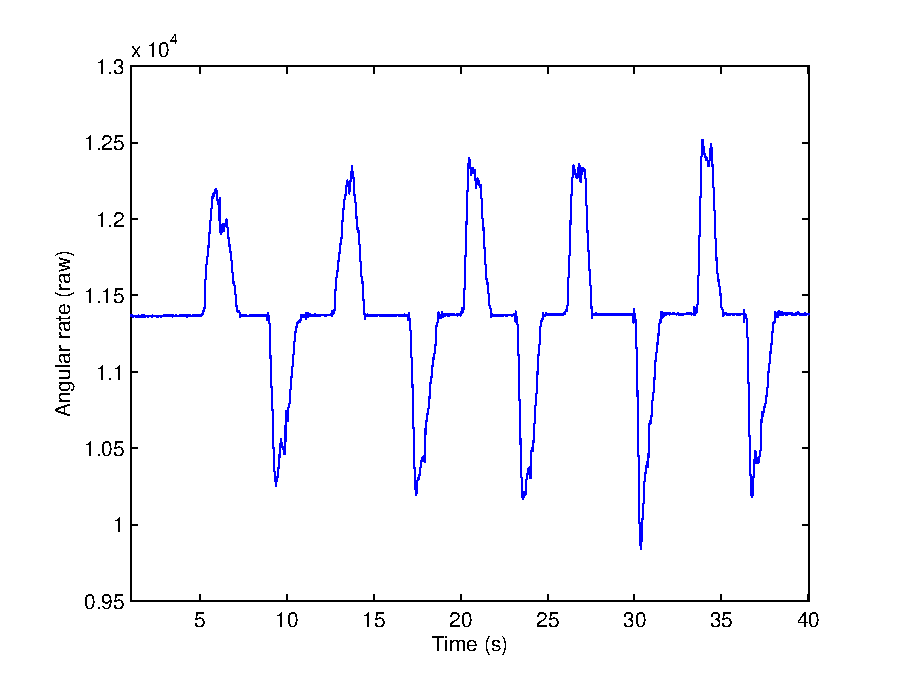
\includegraphics[width=0.7\textwidth]{figures/gyro_axis_ID_signal.eps}
\caption{Angular rate signal gathered during maneuvers of identification of rotation.}
\label{fig:rotation_axis_sense2}
\end{figure}

This procedure needs to be repeated for each one of the axis of the gyroscopes located in all the units. \\
\indent Table \ref{tab:gyro_channels} shows the channels of all GaitWatch's gyroscopes.

\begin{table}[H]
\caption{List of Gaitwatch's gyroscopes and their associated channels.}
	\centering
		\begin{tabular}{|c|c|c|c|}\hline
		\label{tab:gyro_channels}
		Unit 				& Axis 	& Sense compensation 	& Channel 	\\ \hline
		Right shank & Y			& Yes (-1)						& 1					\\
		Right thigh & Y			& Yes (-1)						& 4					\\
		Left shank  & Y			& Yes (-1)						& 7					\\
		Left thigh  & Y			& Yes (-1)						& 10				\\
		Left arm		& Y			& No  (+1)						& 13				\\
		Left arm		& X			& Yes (-1)						& 14				\\
		Right arm		& Y			& No  (+1)						& 15				\\
		Right arm		& X			& Yes (-1)						& 16				\\
		Trunk				& Z			& No	(+1)						& 17				\\
		Trunk				& Y			& No	(+1)						& 18				\\	
		Trunk				& X			& Yes	(-1)						& 19				\\ \hline
		\end{tabular}
\end{table}

\subsection{Identification of Magnetometer's axes}
\label{subsec:mag_ID}

\indent \indent The data of the triaxial magnetometer embedded in the trunk unit are all contained in the same channel (channel 23). Each axis data has a different offset so it is easy to separate them. The axes offsets are +32764, 20000 and 0. Once we have separated the data, we need to identify which axis corresponds to each offset. To do so, we place the desired axis pointing upwards or downwards and turn the box more than 360 degrees. Then, the signal corresponding to the selected axis should be the one showing the least variation (as it is shown in figure \ref{fig:mag_axis_ID}). This operation needs to be repeated two more times to identify the remaining two axes. 
\begin{table}[H]
\caption{Magnetometer's offsets and axes.}
	\centering
		\begin{tabular}{|c|c|c|}\hline
		\label{tab:mag_offsets}
		Unit		& Axis 	& Offset 	\\ \hline
		Trunk		& X			& -20000				\\ 
		Trunk		& Y			& 0	\\ 
		Trunk		& Z			& +32764	\\ \hline
		\end{tabular}
\end{table}

\begin{figure}[H]
\centering
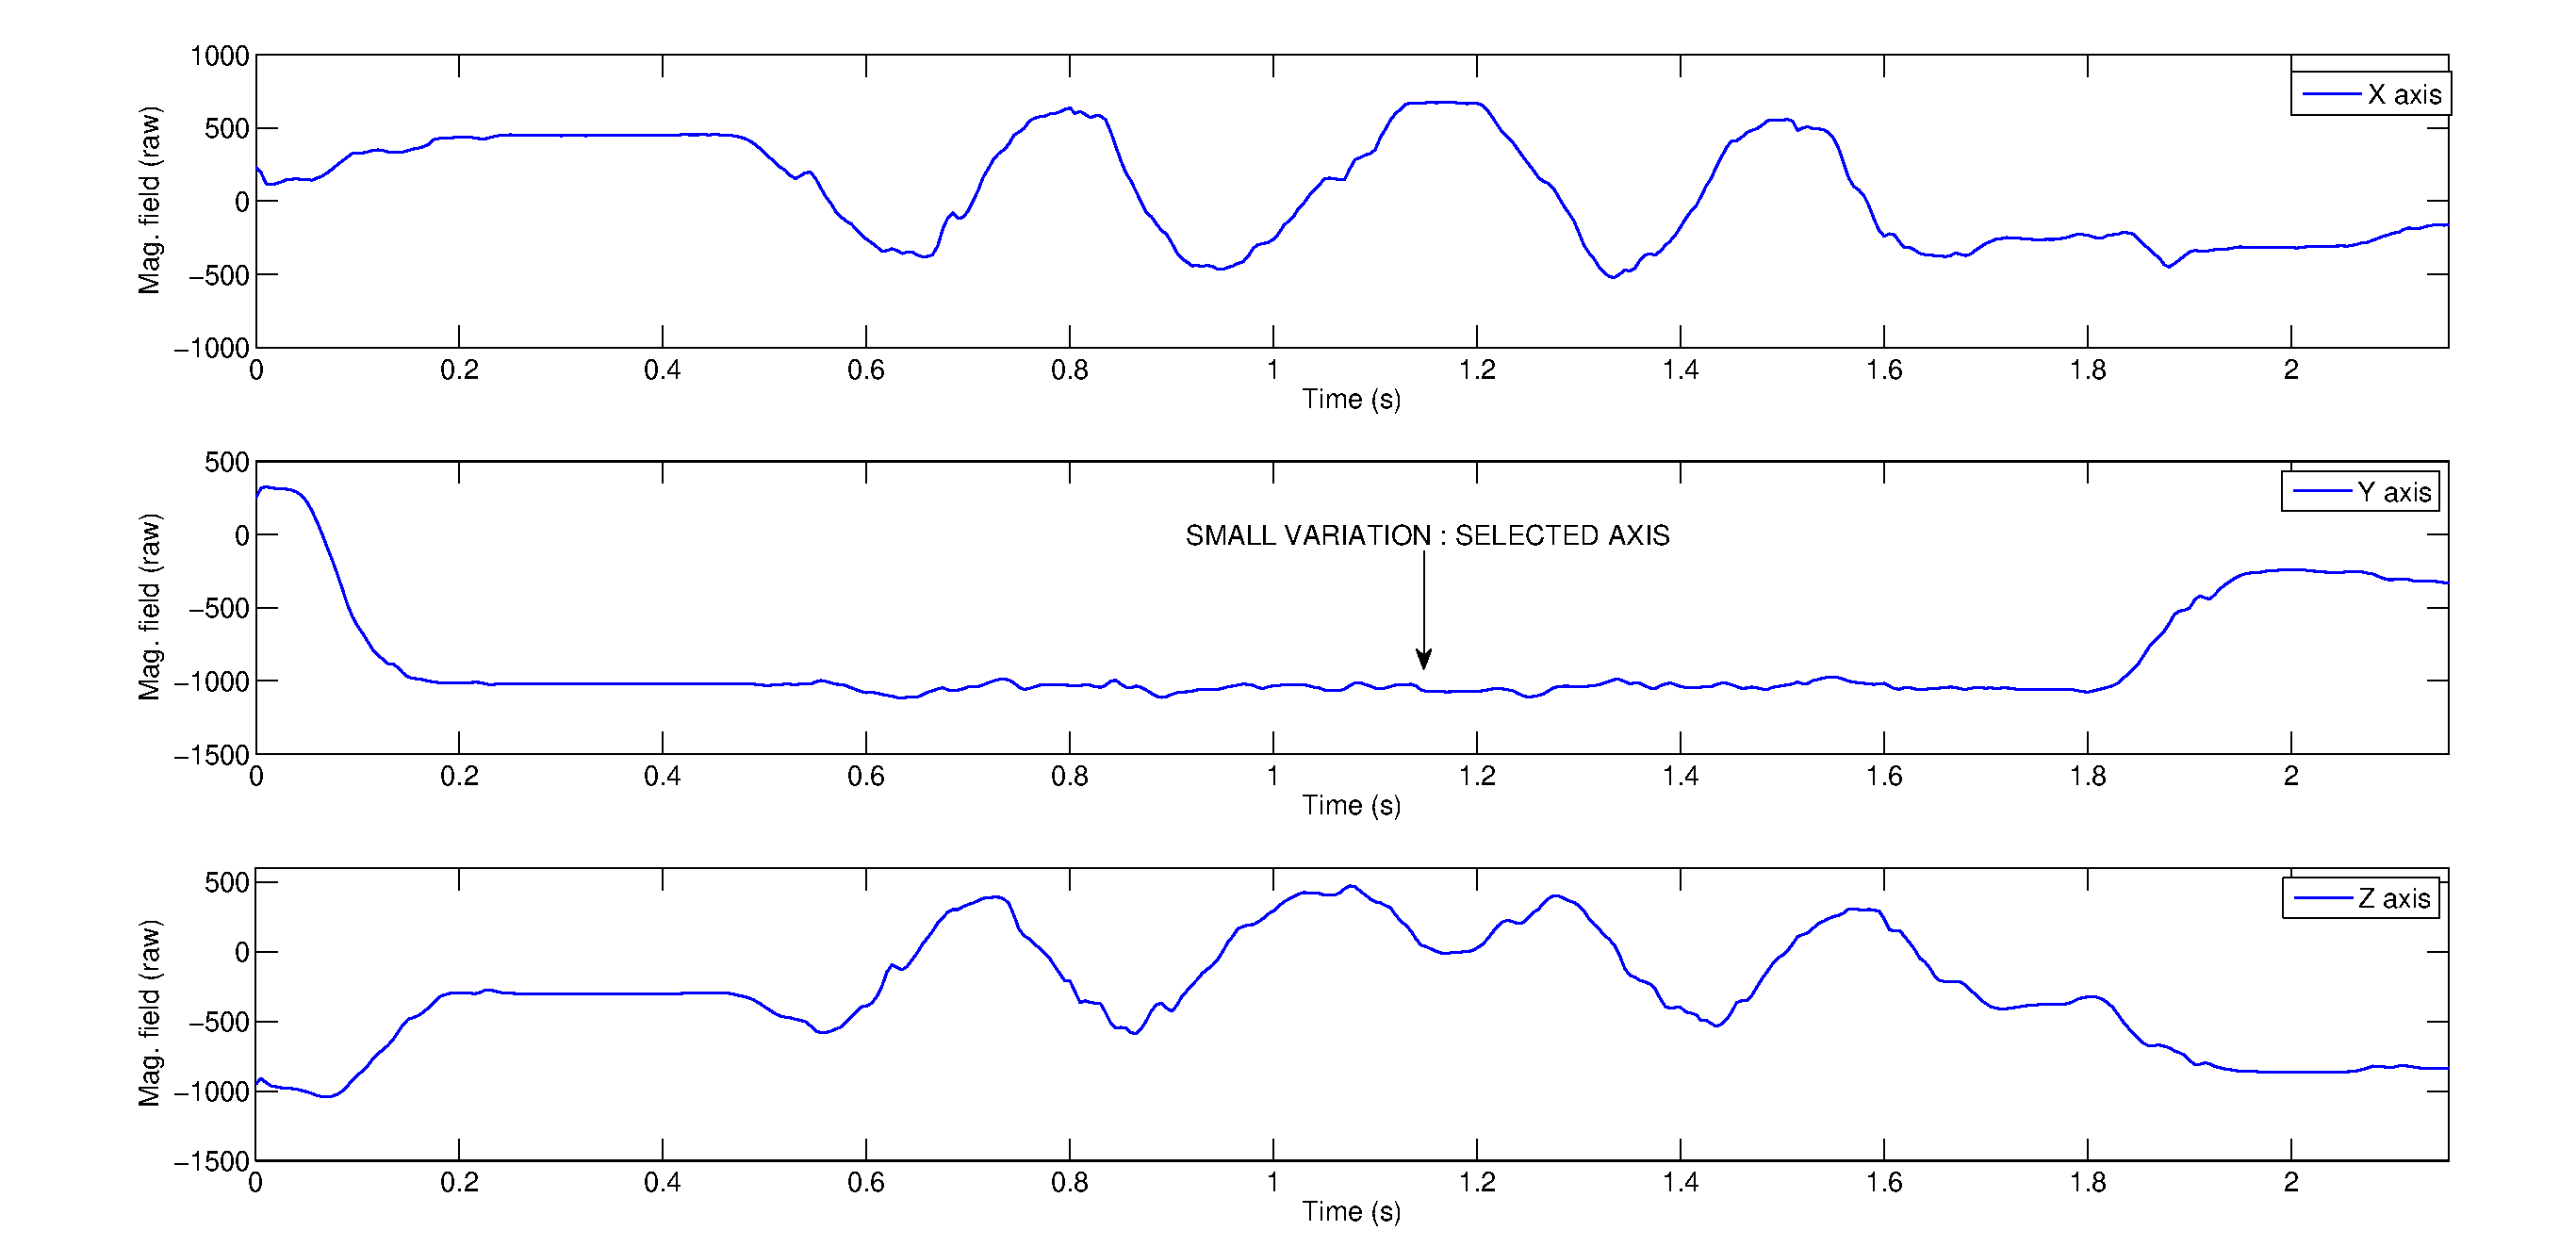
\includegraphics[width=1\textwidth]{figures/mag_axis_ID.eps}
\caption{Magnetic field signal gathered during maneuvers of Z axis identification.}
\label{fig:mag_axis_ID}
\end{figure}


	\clearemptydoublepage
	\chapter{Calibration of sensors}
\label{ch:calibration}

\indent \indent Once the axes are properly identified, the next step is to calibrate all its sensors. The main goal of the calibration process is to transform the raw data into meaningful physical units. 

\subsection{Accelerometer calibration}
\label{subsec:acc_calibration}

\indent \indent The calibration of the accelerometers is divided in two parts according to the number of axes of the accelerometer. For the triaxial accelerometer included in the trunk unit (the box) we will use the ellipsoid fitting algorithm by Camps et al. \cite{camps_numerical_2009}. They present a theoretical and experimental method to compute gains, bias and non orthogonality factors of magnetometer and acce\-le\-ro\-me\-ter sensors. The calibration procedure involves arbitrary rotations of the MIMU, so the set of maneuvers to gather the necessary data is very simple.
\begin{itemize}
\item \textbf{Sensor Modeling}: The model of the sensor output is given by:
    \begin{equation}
    \left[
      \begin{array}{c}
        \mbox{v}_{\scriptsize \mbox{x}}(t) \\
        \mbox{v}_{\scriptsize \mbox{y}}(t) \\
        \mbox{v}_{\scriptsize \mbox{z}}(t) \\
      \end{array}
    \right]=\left[
              \begin{array}{ccc}
                \mbox{s}_{\scriptsize \mbox{x}} & 0 & 0 \\
                0 & \mbox{s}_{\scriptsize \mbox{y}} & 0 \\
                0 & 0 & \mbox{s}_{\scriptsize \mbox{z}} \\
              \end{array}
            \right]\left[
                     \begin{array}{c}
                       \mbox{m}_{\scriptsize \mbox{x}}(t) \\
                       \mbox{m}_{\scriptsize \mbox{y}}(t) \\
                       \mbox{m}_{\scriptsize \mbox{z}}(t) \\
                     \end{array}
                   \right]+\left[
                             \begin{array}{c}
                               \mbox{b}_{\scriptsize \mbox{x}} \\
                               \mbox{b}_{\scriptsize \mbox{y}} \\
                               \mbox{b}_{\scriptsize \mbox{z}} \\
                             \end{array}
                           \right]+\left[
                                     \begin{array}{c}
                                       \varepsilon_{\scriptsize \mbox{x}} \\
                                       \varepsilon_{\scriptsize \mbox{y}} \\
                                       \varepsilon_{\scriptsize \mbox{z}} \\
                                     \end{array}
                                   \right]
    \label{eq:CampsModel}
    \end{equation}
    where $\mathbf{b}=(\mbox{b}_{\scriptsize \mbox{x}}, \mbox{b}_{\scriptsize \mbox{y}}, \mbox{b}_{\scriptsize \mbox{z}})^{T}$ represents the offset, $\mbox{s}_{\scriptsize \mbox{x}}$, $\mbox{s}_{\scriptsize \mbox{y}}$, $\mbox{s}_{\scriptsize \mbox{z}}$ are the sensor gains, $\mbox{m}_{\scriptsize \mbox{x}}(t)$, $\mbox{m}_{\scriptsize \mbox{y}}(t)$, $\mbox{m}_{\scriptsize \mbox{z}}(t)$ are the components of the actual magnetic field or gravity and $\varepsilon_{x}$, $\varepsilon_{y}$, $\varepsilon_{z}$ are the components of the noise for each axis. \\
    \indent If we take into consideration the effects of non-orthogonality, then the sensor output is given by:
    \begin{equation}
    \left[
      \begin{array}{c}
        \mbox{v}_{\scriptsize \mbox{x}}(t) \\
        \mbox{v}_{\scriptsize \mbox{y}}(t) \\
        \mbox{v}_{\scriptsize \mbox{z}}(t) \\
      \end{array}
    \right]=\left[
              \begin{array}{ccc}
                \mbox{s}_{\scriptsize \mbox{xx}} & s_{\scriptsize \mbox{xy}} & s_{\scriptsize \mbox{xz}} \\
                \mbox{s}_{\scriptsize \mbox{xy}} & s_{\scriptsize \mbox{yy}} & s_{\scriptsize \mbox{yz}} \\
                \mbox{s}_{\scriptsize \mbox{xz}} & s_{\scriptsize \mbox{yz}} & s_{\scriptsize \mbox{zz}} \\
              \end{array}
            \right]\left[
                     \begin{array}{c}
                       \mbox{m}_{\scriptsize \mbox{x}}(t) \\
                       \mbox{m}_{\scriptsize \mbox{y}}(t) \\
                       \mbox{m}_{\scriptsize \mbox{z}}(t) \\
                     \end{array}
                   \right]+\left[
                             \begin{array}{c}
                               \mbox{b}_{\scriptsize \mbox{x}} \\
                               \mbox{b}_{\scriptsize \mbox{y}} \\
                               \mbox{b}_{\scriptsize \mbox{z}} \\
                             \end{array}
                           \right]+\left[
                                     \begin{array}{c}
                                       \varepsilon_{\scriptsize \mbox{x}} \\
                                       \varepsilon_{\scriptsize \mbox{y}} \\
                                       \varepsilon_{\scriptsize \mbox{z}} \\
                                     \end{array}
                                   \right]
    \label{eq:CampsModel2}
    \end{equation}
    where $\mbox{s}_{ij}$ for $i\neq j$ represent the orthogonality errors between sensor axes $i$ and $j$.

\item \textbf{Calibration Procedure}: Using the fact that the norm of the input vector $\mathbf{m}=[\mbox{m}_{\scriptsize \mbox{x}}(t)\quad \mbox{m}_{\scriptsize \mbox{y}}(t) \quad \mbox{m}_{\scriptsize \mbox{z}}(t)]^{T}$ is constant, the following relation is derived:
    \begin{equation}
    \|\mathbf{m}\|^{2}=\mbox{m}_{\scriptsize \mbox{x}}(t)^{2}+\mbox{m}_{\scriptsize \mbox{y}}(t)^{2}+\mbox{m}_{\scriptsize \mbox{z}}(t)^{2}
    \label{eq:CampsGeneral}
    \end{equation}
    \begin{equation}
    \|\mathbf{h}\|^{2}=\left(\frac{\mbox{v}_{\scriptsize \mbox{x}}(t)-\mbox{b}_{\scriptsize \mbox{x}}}{\mbox{s}_{\scriptsize \mbox{x}}}\right)^{2}+\left(\frac{\mbox{v}_{\scriptsize \mbox{y}}(t)-\mbox{b}_{\scriptsize \mbox{y}}}{\mbox{s}_{\scriptsize \mbox{y}}}\right)^{2}+\left(\frac{\mbox{v}_{\scriptsize \mbox{z}}(t)-\mbox{b}_{\scriptsize \mbox{z}}}{\mbox{s}_{\scriptsize \mbox{z}}}\right)^{2}
    \label{eq:CampsEllip}
    \end{equation}
    Equation (\ref{eq:CampsEllip}) is the parametric equation of an ellipsoid with center $\mathbf{b}$ and semi-axes $\mbox{s}_{\scriptsize \mbox{x}}, \mbox{s}_{\scriptsize \mbox{y}}$ and $\mbox{s}_{\scriptsize \mbox{z}}$. Using the system of equations formed by the various measurements at times t, we estimate the parameters through non-linear least squares minimization of the error function
    \begin{equation}
    e_{\scriptsize \mbox{p}}(t)=\|\mathbf{m}\|^{2}-\left(\mathbf{v}(t)-\mathbf{b}\right)^{T}\left(\mbox{S}^{-1}\right)^{2}\left(\mathbf{v}(t)-\mathbf{b}\right)
    \label{eq:CampsError}
    \end{equation}
    where
    \begin{equation}
    \mbox{S}^{-1}=\left[
              \begin{array}{ccc}
                1/\mbox{s}_{\scriptsize \mbox{xx}} & 1/\mbox{s}_{\scriptsize \mbox{xy}} & 1/\mbox{s}_{\scriptsize \mbox{xz}} \\
                1/\mbox{s}_{\scriptsize \mbox{xy}} & 1/\mbox{s}_{\scriptsize \mbox{yy}} & 1/\mbox{s}_{\scriptsize \mbox{yz}} \\
                1/\mbox{s}_{\scriptsize \mbox{xz}} & 1/\mbox{s}_{\scriptsize \mbox{yz}} & 1/\mbox{s}_{\scriptsize \mbox{zz}} \\
              \end{array}
            \right]
    \label{eq:CampsS}
    \end{equation}
    The cost function $e_{\scriptsize \mbox{p}}(t)$ is quadratic, and is minimized iteratively by the \emph{Le\-ven\-berg\--Mar\-quardt} algorithm (LMA) \cite{Levenberg,Marquardt}.
\end{itemize}

Long story short, if the accelerometer is placed in multiple random quasi-static positions, the gathered data should ideally describe an sphere of radius equal to the magnitude of the gravity vector. \\
\indent Therefore, the first calibration step is to gather the acceleration data which will be used to find the optimal calibration parameters. As it is said before, we need to place the unit containing the accelerometer in multiple random quasi-static positions. To do so, we put the box in a set of random positions trying to cover all the orientations. Since the transitions from one quasi-static position to other cause the accelerometer to measure linear acceleration which disrupt the gravity acceleration, we can not just take every measured point but we need to apply an algorithm which is able to detect the quasi-static instants. \\
Figure \ref{fig:acc_multiposition_signals} show the triaxial acceleration measured in each quasi-static position in addition to the undesired linear acceleration. This figure also shows the output of the quasi-static instant detection algorithm. 

\begin{figure}[H]
\centering
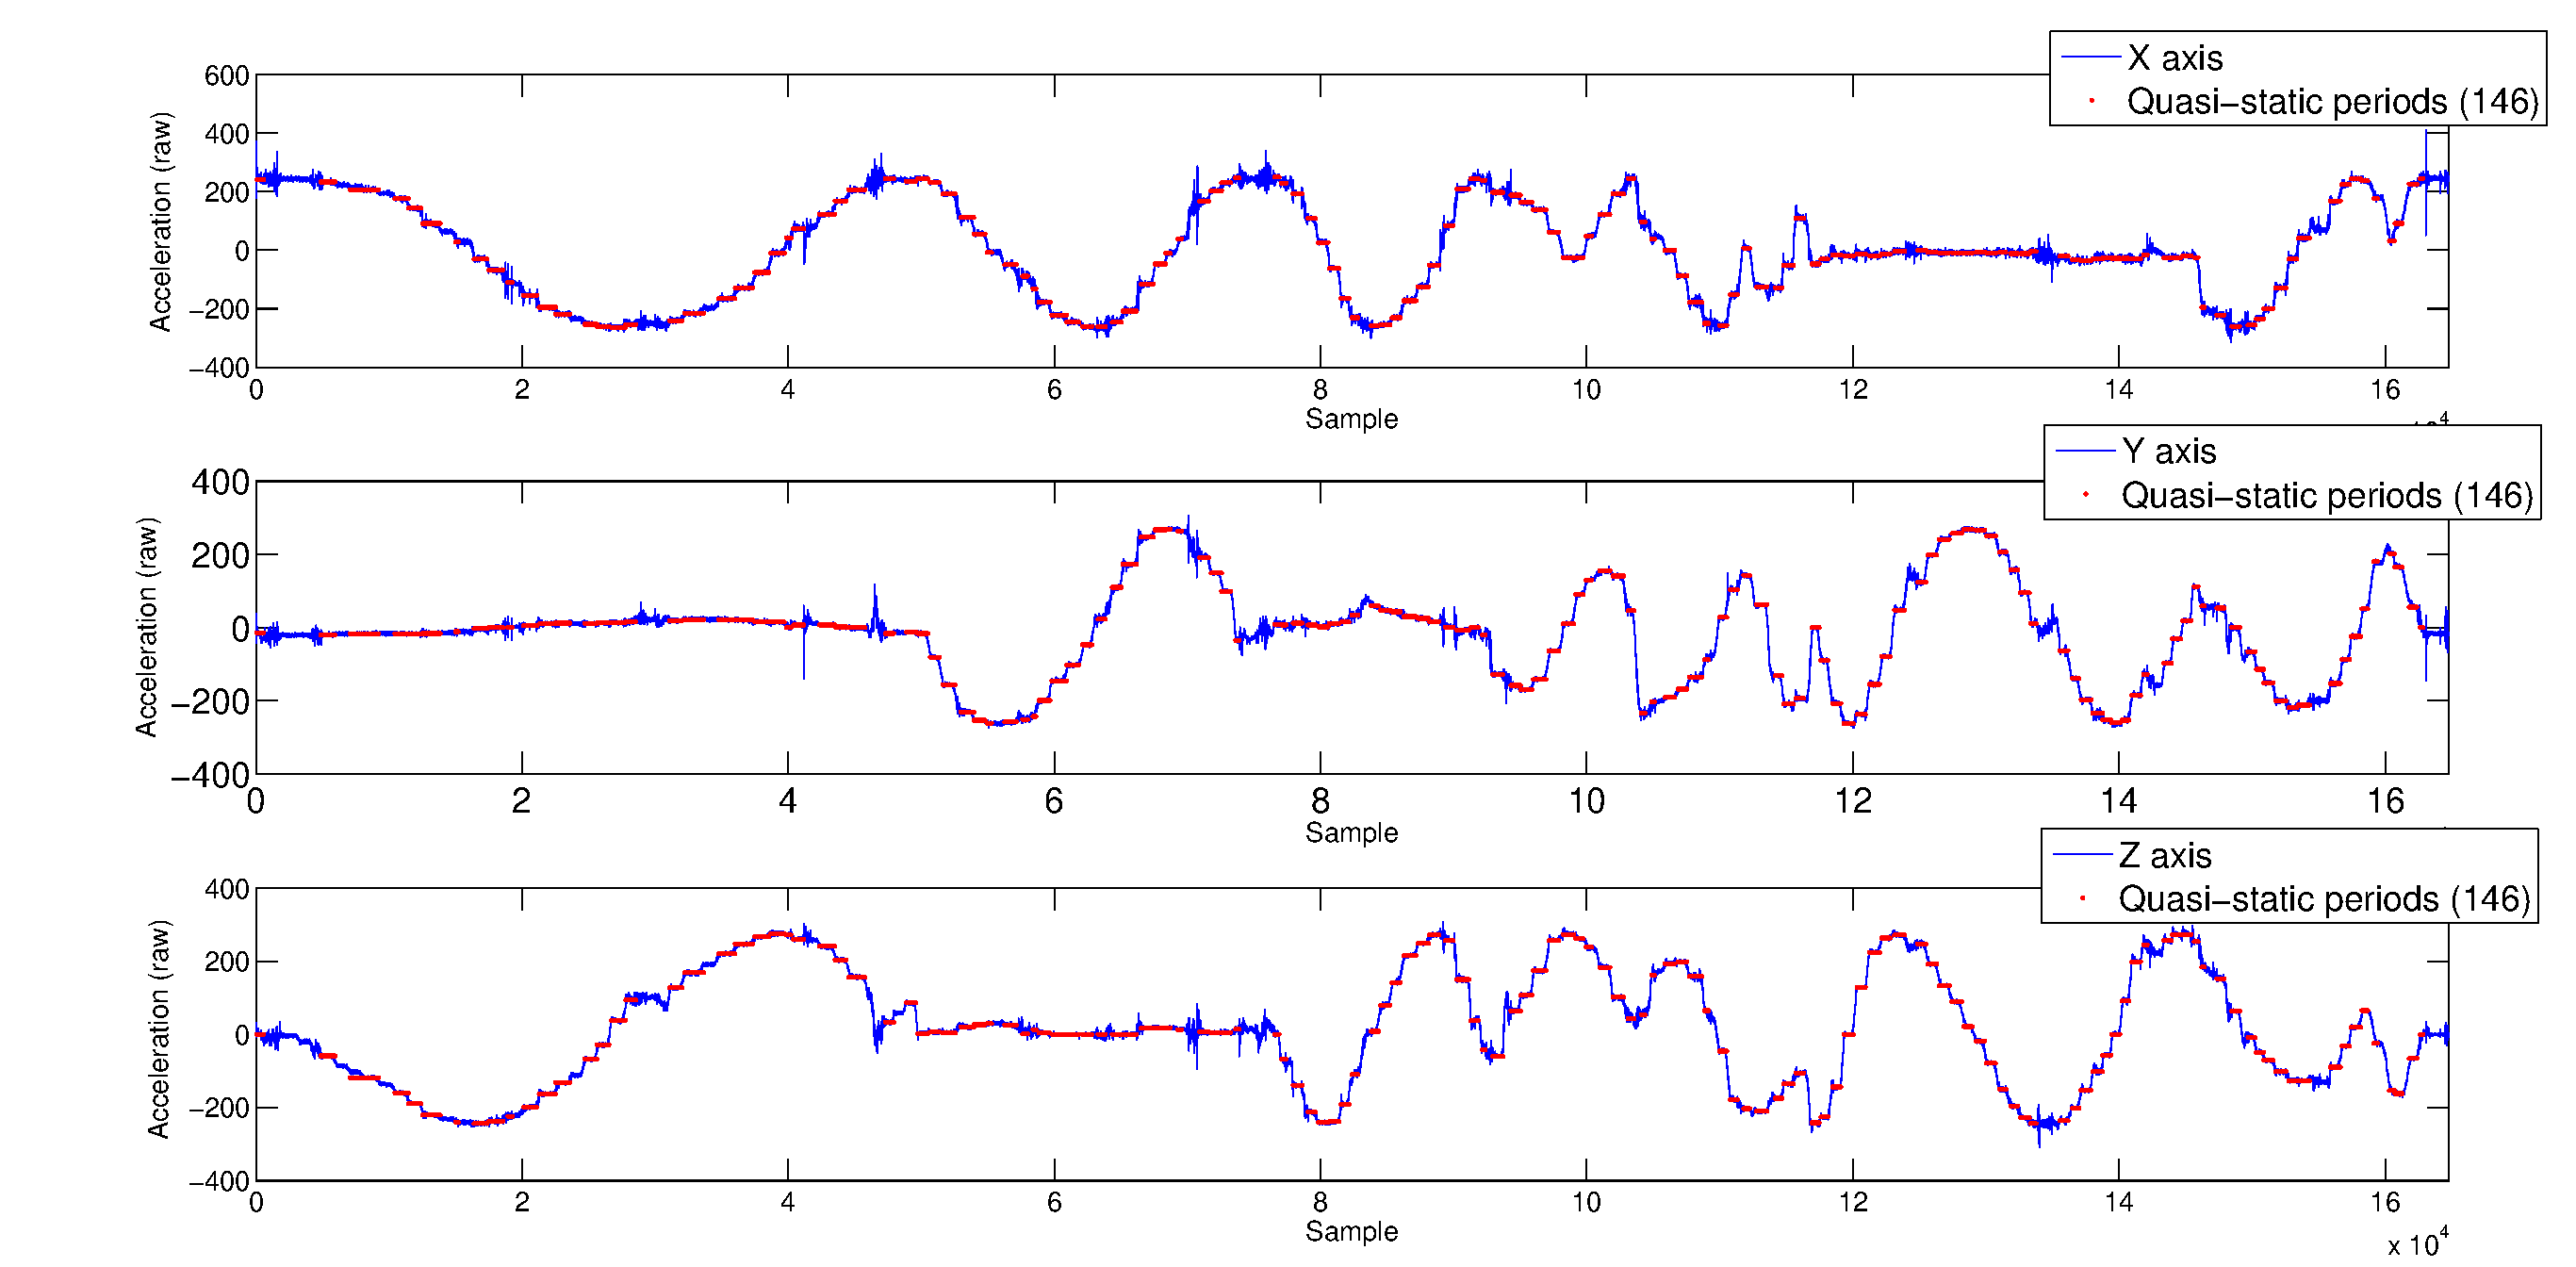
\includegraphics[width=1\textwidth]{figures/acc_multiposition_signals.eps}
\caption{Acceleration gathered during quasi-static positions and output of the detection algorithm}
\label{fig:acc_multiposition_signals}
\end{figure}

If we plot the detected quasi-static accelerations in 3D, they should cover the locus of a sphere as it is shown in figure \ref{fig:acc_multiposition_3D}

\begin{figure}[H]
\centering
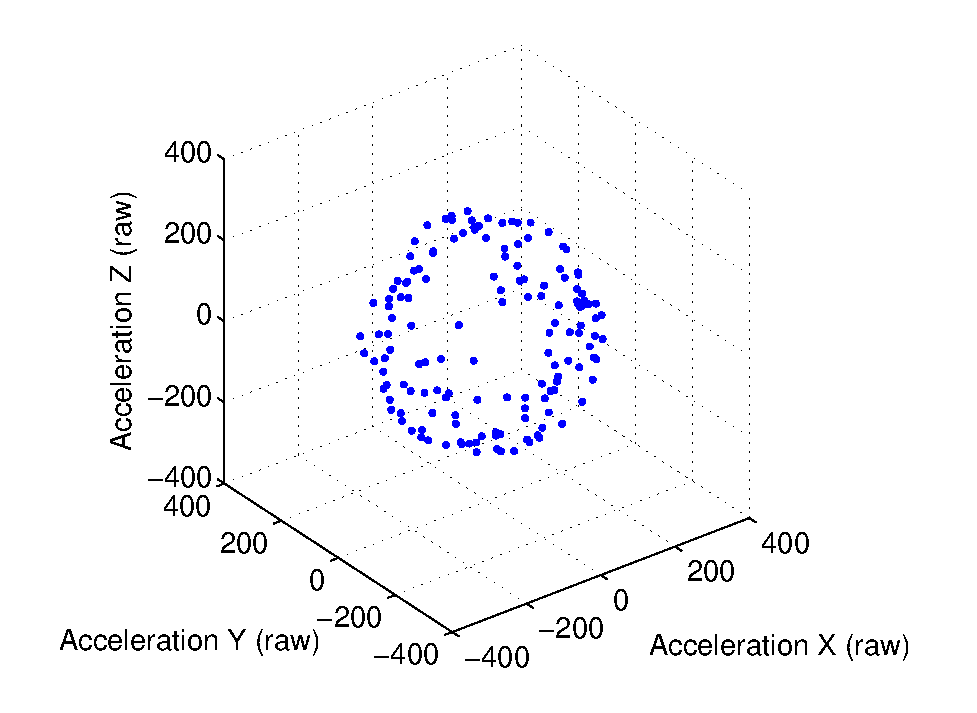
\includegraphics[width=0.6\textwidth]{figures/acc_multiposition_3D.eps}
\caption{3D representation of acceleration gathered during quasi-static positions.}
\label{fig:acc_multiposition_3D}
\end{figure}

We then feed the algorithm with these data and the calibration parameters are found. Equation \ref{eq:trunk_acc_params} shows the estimated calibration parameters for the trunk triaxial accelerometer.

\begin{gather}
\label{eq:trunk_acc_params}
S = \left[\begin{array}{ccc}
		256.68 						& -4.01\cdot10^{-5} & -2.41\cdot10^{-5} \\
		-4.01\cdot10^{-5}	&	262.74						&	-3.98\cdot10^{-7} \\
		-2.41\cdot10^{-5}	& -3.98\cdot10^{-7}	& 263.04 \\
		\end{array}\right] \\ \nonumber
\mathbf{b} = \left[-23.69\quad -6.95\quad 22.85\right]
\end{gather}

These parameters are then plugged in the following equation to obtain the calibrated triaxial acceleration:

\begin{equation}
\label{eq:cal_acceleration}
\mathbf{a}_{cal}=S^{-1}(\mathbf{a}_{raw}-\mathbf{b})
\end{equation}

where $\mathbf{a}_{cal}$ is a three dimensional vector containing the calibrated acceleration, S is the computed orthogonality matrix, $\mathbf{a}_{raw}$ is the three dimensional vector containing the raw acceleration and $\mathbf{b}$ is the computed triaxial bias vector.

Figure \ref{fig:acc_multiposition_cal_3D_4POV} shows the calibrated quasi-static accelerations. Notice how the points define now a sphere centered in the origin with a radius of 1(g).

\begin{figure}[H]
\centering
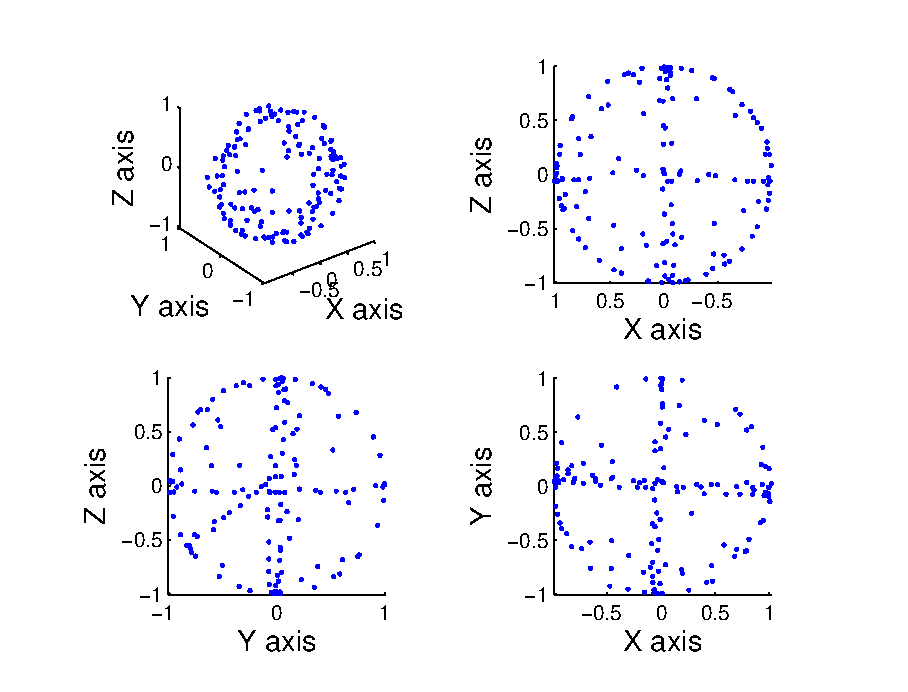
\includegraphics[width=0.8\textwidth]{figures/acc_multiposition_cal_3D_4POV.eps}
\caption{3D representation of calibrated quasi-static positions.}
\label{fig:acc_multiposition_cal_3D_4POV}
\end{figure}

For the biaxial accelerometer we could adapt the method aforementioned to two dimensions. However, the calibration maneuvers would be much more complicated since we would need to lock the unit including the accelerometer in the XZ plane and then describe a complete slow rotation to gather the quasi-static positions. \\

\indent We opted to carry out a single-axis calibration procedure which only requires to gather data from two positions for each axis. This procedure is very simple; we first set the desired axis parallel to the gravity vector and leave it in that position for a couple of seconds and we then flip it so it is anti-parallel to the gravity vector and leave it static again for another two seconds. Proceeding this way, we know the raw values corresponding to +1g and -1g respectively. Since the accelerometers included in GaitWatch's units are linear, we can then find the calibration equation in a very simple way. The calibration equation is defined as follows,

\begin{equation}
\label{eq:acc_1D_cal_equation}
a_{cal} = k\cdot a_{raw} + b
\end{equation}

where $a_{cal}$ is the calibrated acceleration, $a_{raw}$ is the raw acceleration, $k$ is the scale factor and $b$ is the bias. If we substitute the two gathered values we would have the following system of equations from which it is straight forward to find the values of $k$ and $b$,

\begin{gather}
\label{eq:acc_1D_cal_system}
1 = k\cdot a_{raw,+} + b \\ \nonumber
-1 = k\cdot a_{raw,-} + b
\end{gather}

where $a_{raw,+}$ and $a_{raw,-}$ are the gathered raw accelerations in the parallel and anti-parallel positions respectively. \\

\indent The units placed on the shanks and the thighs contain a biaxial accelerometer (X,Z) so we can put the unit in the four required positions (two for each axis) and then apply the quasi-static positions detector to extract the values in these positions. \\

\indent Figure \ref{fig:acc_raw_4_positions} shows the gathered raw acceleration in such four positions and the extracted quasi-static values for the accelerometer in the left shank unit. 

\begin{figure}[t]
\centering
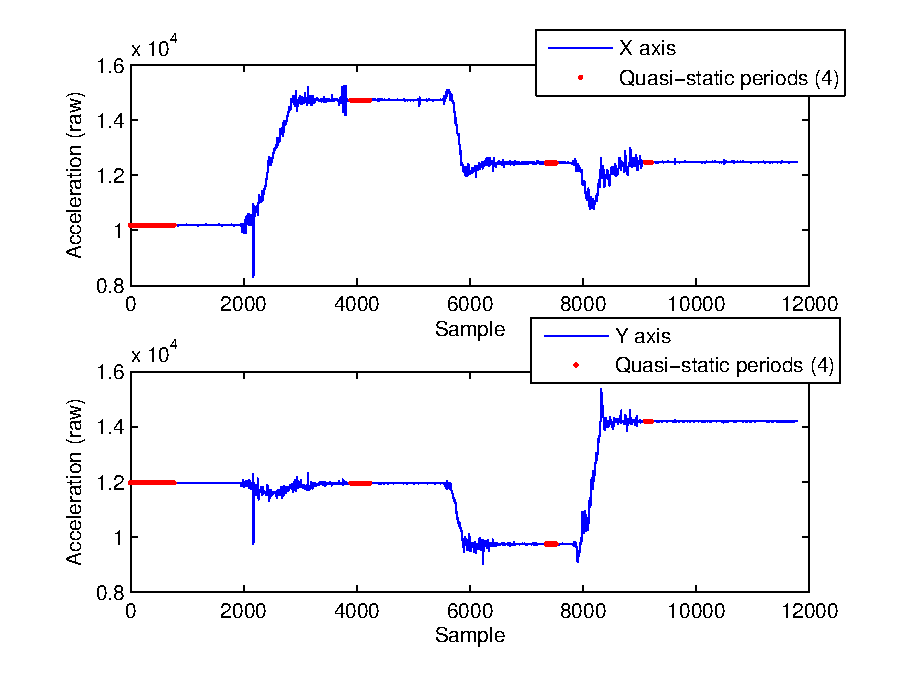
\includegraphics[width=0.8\textwidth]{figures/acc_raw_4_positions.eps}
\caption{Raw acceleration gathered when both axes X and Z are placed parallel and anti-parallel to the gravity vector.}
\label{fig:acc_raw_4_positions}
\end{figure}

Using this procedure the calibration parameters are found for all the units. Table \ref{tab:acc2D_cal_params} shows them. 

\begin{table}[H]\footnotesize
\caption{Calibration parameters of biaxial accelerometers (valid as of December the 10th, 2013).}
	\centering
		\begin{tabular}{|c|c|c|c|}\hline
		\label{tab:acc2D_cal_params}
		Unit				& Axis 	& Scale factor 	& Bias 	\\ \hline
		Left shank 	& X			& 4.45e-04			& -5.59 \\
		Left shank 	& Z			& 4.49e-04			& -5.36 \\
		Left thigh	& X			& 4.58e-04			& -5.76 \\
		Left thigh	& Z			& 4.74e-04			& -5.70 \\
		Right shank & X			& 4.38e-04			& -5.50 \\
		Right shank & Z			& 4.77e-04			& -5.72 \\
		Right thigh & X			& 4.36e-04			& -5.44 \\
		Right thigh & Z			& 4.43e-04			& -5.34 \\ \hline
		\end{tabular}
\end{table}

\subsection{Magnetometer calibration}
\label{subsec:mag_calibration}

\indent \indent The calibration of the triaxial magnetometer is also based on the algorithm by Camps et al. used for the accelerometer calibration. In this case, we only need to change the data gathering maneuvers and the value of the magnitude of the reference vector (which in this case is the Earth's magnetic field vector).\\

\indent The maneuvers are much simpler in this case since the magnetometer is not affected by the linear acceleration. Therefore, we can freely move the magnetometer at any speed trying to cover the most possible space. Figure \ref{fig:mag_raw_3D} shows the 3D representation of the raw magnetic field measured carrying these maneuvers. 

\begin{figure}[t]
\centering
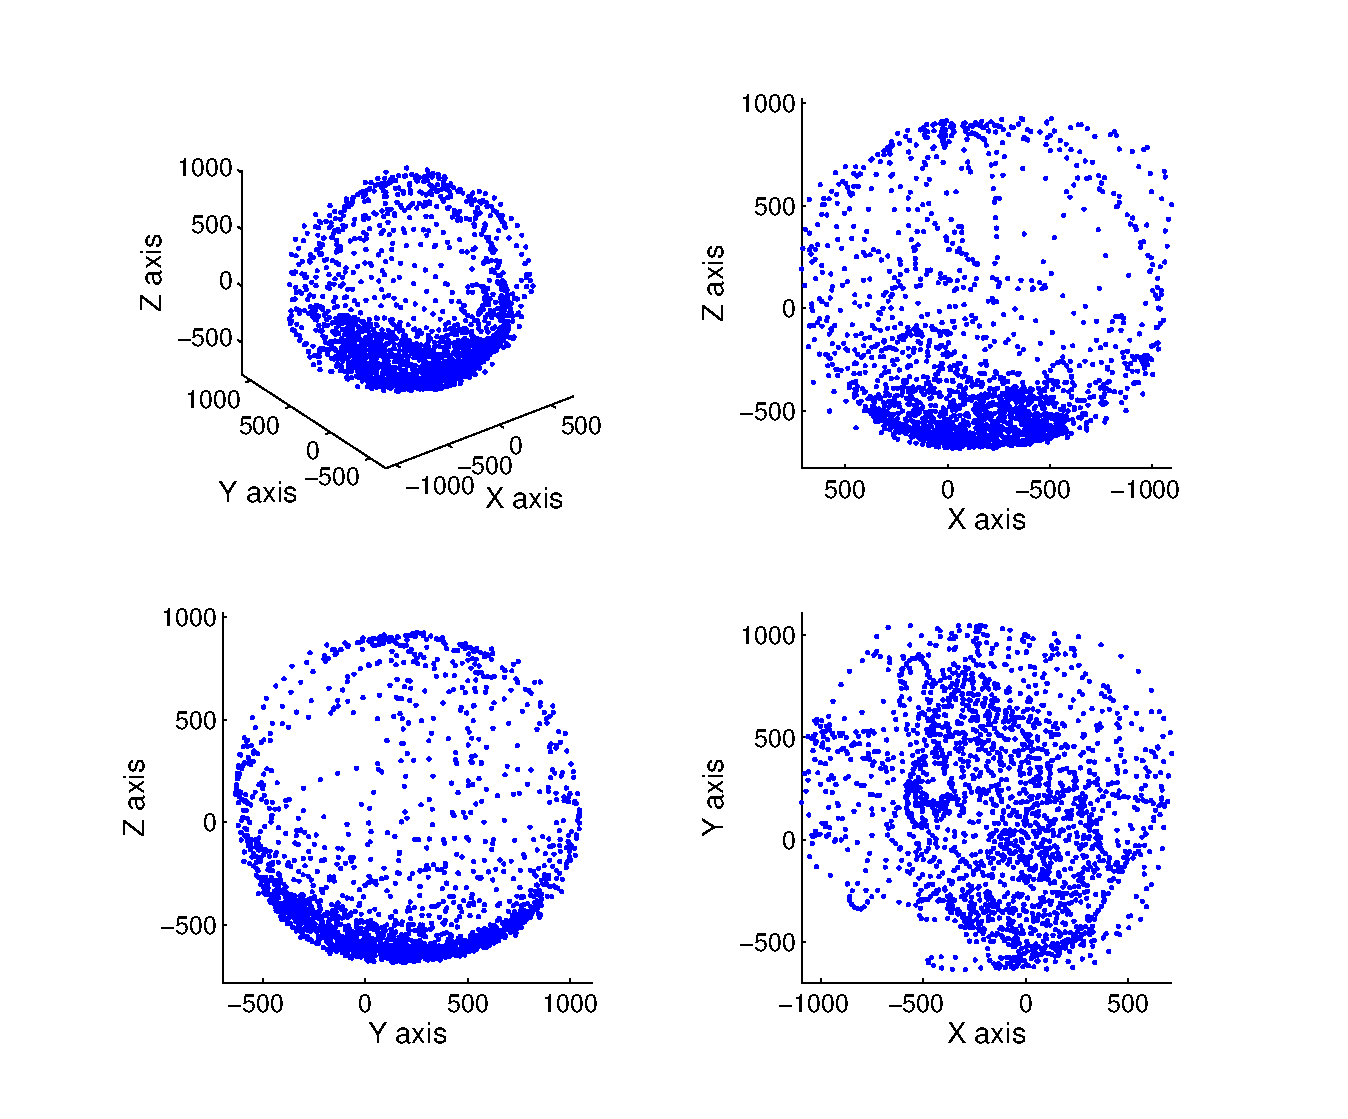
\includegraphics[width=0.8\textwidth]{figures/trunk_rawMag3D_4POV.eps}
\caption{Raw magnetic field gathered by randomly moving the trunk unit containing the magnetometer.}
\label{fig:mag_raw_3D}
\end{figure}

Ideally, these data should describe an sphere centered in the origin with a radius given by the magnitude of the local Earth's magnetic field. By checking the Magnetic field calculator from the American National Geophysical Data Center \cite{center_ngdc}, we can obtain the value for Munich, which is 0.482352 Gauss. We then feed the algorithm with the data shown in figure \ref{fig:mag_raw_3D} and the calibration parameters are computed. Analogously to the accelerometer, the calibrated magnetic field is found applying the following equation,

\begin{equation}
\label{eq:cal_mag}
\mathbf{h}_{cal}=S^{-1}(\mathbf{h}_{raw}-\mathbf{b})
\end{equation}

where again $\mathbf{h}_{cal}$ is a three dimensional vector containing the calibrated magnetic field, S is the computed orthogonality matrix, $\mathbf{h}_{raw}$ is the three dimensional vector containing the raw magnetic field and $\mathbf{b}$ is the computed triaxial bias vector. If we apply this equation to the raw values used to compute the parameters, we can see how they now define a sphere centered in 0 and with radius 0.482352 Gauss (figure \ref{fig:mag_cal_3D}).

\begin{figure}[H]
\centering
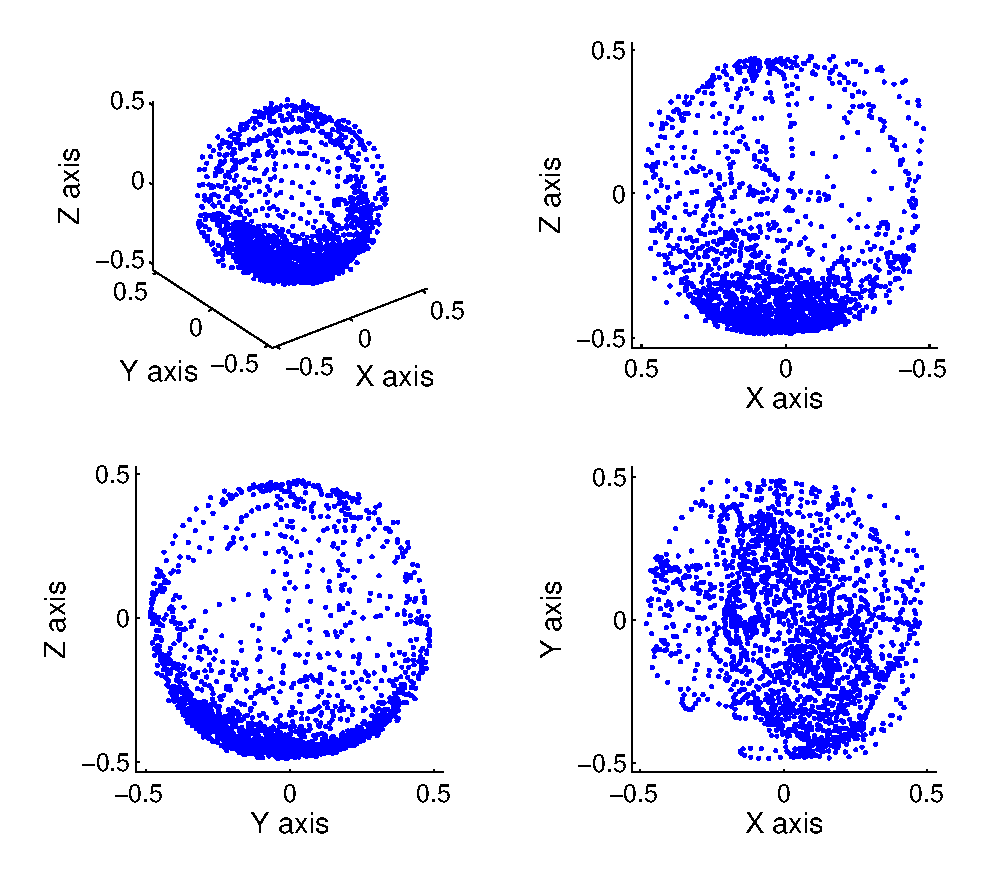
\includegraphics[width=0.5\textwidth]{figures/trunk_calMag3D_4POV.eps}
\caption{Calibrated magnetic field gathered by randomly moving the trunk unit containing the magnetometer.}
\label{fig:mag_cal_3D}
\end{figure}

Figure \ref{fig:trunk_rawVsCal} shows the raw and calibrated signals for all the three axes of the magnetometer included in the trunk's unit.

\begin{figure}[H]
\centering
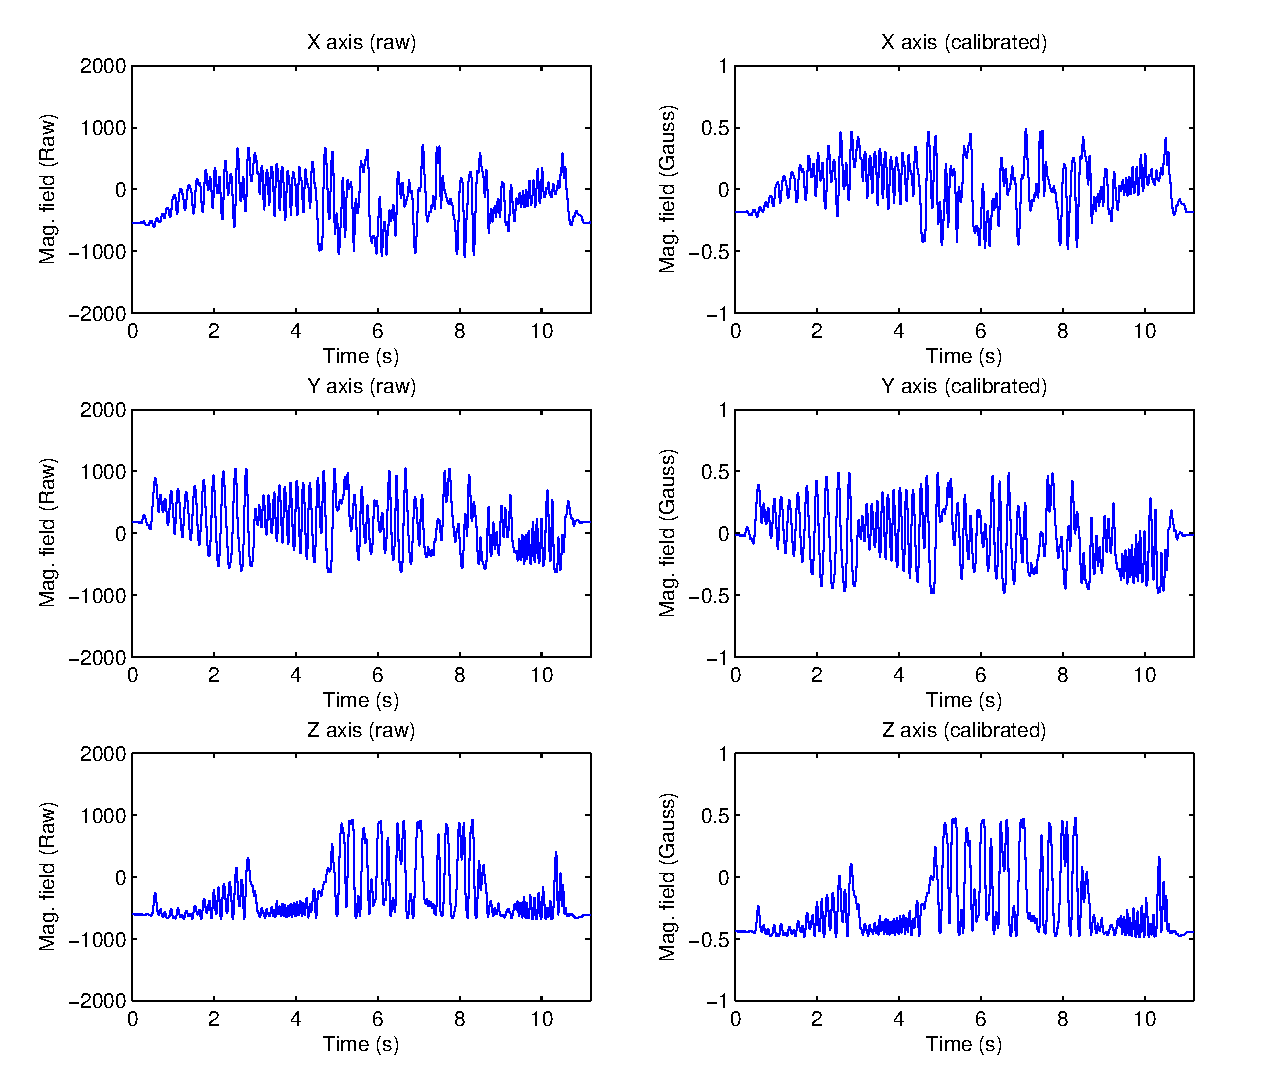
\includegraphics[width=0.7\textwidth]{figures/trunk_rawVsCal.eps}
\caption{Calibrated magnetic field vs. raw magnetic field gathered by randomly moving the trunk unit containing the magnetometer.}
\label{fig:trunk_rawVsCal}
\end{figure}

The calibration parameters (valid as of December the 10th, 2013) of the magnetometer in the trunk unit are listed below 

\begin{gather}
\label{eq:mag_cal_params}
S = \left[\begin{array}{ccc}
		1.75\cdot10^{3} 	& -3.46\cdot10^{-8} & -3.04\cdot10^{-6} \\
		-3.46\cdot10^{-8}	&	1.97\cdot10^{3}	 & 1.42\cdot10^{-5} \\
		-3.04\cdot10^{-5}	& 1.42\cdot10^{-6} & 1.83\cdot10^{3}  \\
		\end{array}\right] \\ \nonumber
\mathbf{b} = \left[14.86\quad 102.43\quad -45.04\right]
\end{gather}

\subsection{Gyroscope calibration}
\label{subsec:gyro_calibration}

\indent \indent The gyroscope is the last remaining kind of sensor to be calibrated. The most accurate way to calibrate a gyroscope is to subject it to different known rotation speeds and then associating them to the raw gathered values to obtain a calibration equation. If a variable rate table is not available, we can use simpler equipment and subject the gyroscope to known rotations instead of known angular rates. To calibrate each one of the axis we need to build a device like the one shown in figure \ref{fig:gyro_turn_device}. This device should allow the rotation of the unit containing the gyroscope around $180^{\circ}$ (other configurations of the device allowing different known rotations are also valid). 

\begin{figure}[H]
\centering
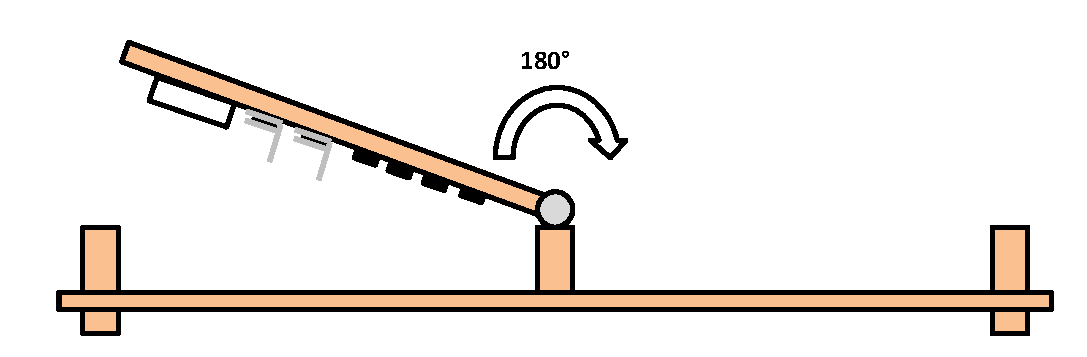
\includegraphics[width=0.8\textwidth]{figures/gyro_turn_device}
\caption{Gyroscope calibration device.}
\label{fig:gyro_turn_device}
\end{figure}

Once the calibration device is ready, the calibration maneuvers are not complicated. Each of the units should be attached to the surface of the device and then we need to carry out a set of $180^{\circ}$ rotations (at least 5). \\

\indent To compute the calibration parameters we are going to use the fact that the integration of the angular speed leads to an angle displacement. Therefore, if we subject the gyroscope to a known rotation ($180^{\circ}$ degrees in this case), we can apply the following equations to find the scale factor,

\begin{gather}
u_{raw} = k\cdot \omega + b \label{eq:gyro_cal1}\\
\omega = \frac{u_{raw}-b}{k} \label{eq:gyro_cal2}\\
u_{raw,corr} = u_{raw}-b \label{eq:gyro_cal3}\\
\int{\omega dt} = \frac{\int{u_{raw,corr} dt}}{k} \label{eq:gyro_cal4}\\
\Omega = \int{\omega dt} \label{eq:gyro_cal5}\\
\theta = \int{u_{raw,corr} dt} \label{eq:gyro_cal6}\\
\Omega = \frac{\theta}{k} \label{eq:gyro_cal7}\\
k = \frac{\theta}{\Omega} \label{eq:gyro_cal8}\\
\end{gather}

\noindent where $u_{raw}$ is the raw gathered angular rate, $\omega$ is the actual angular rate (in physical units), $k$ is the scale factor and $b$ is the bias. In this case $\Omega = 180^{\circ}$ and $\theta$ is the integrated raw gathered angular rate (corrected in bias) during the rotation of $180^{\circ}$. We can see that prior to the integration of the raw angular rate we need to subtract the bias. \\

The bias is easily found by leaving the units in a static position before starting the rotation and then visually inspecting the gathered signal. To take into account the effects of noise, we compute the mode of all the samples gathered while the sensors are static. \\

From a practical point of view, the Matlab calibration routine first displays the gathered raw angular rate signal and asks the user to select the initial and final points of the static period as it is shown in figure \ref{fig:gyro_cal_routine_bias}.

Once the bias is found, we need to tell the routine each one of the starting and ending points of the rotations so it knows the initial and final time instants of the integration. To do so we use the \textit{datacursor}. It is important to only select the positive rotations (as indicated in figure \ref{fig:gyro_cal_routine_sf}), that is, those in which the angular rate first increases and then decreases. The routine will then integrate the selected segments of the signal and average the computed scale factor for each one of them. 

The calibrated angular rate is finally found by substituting the computed calibration parameters in equation (\ref{eq:gyro_cal2}).

\begin{figure}[H]
\centering
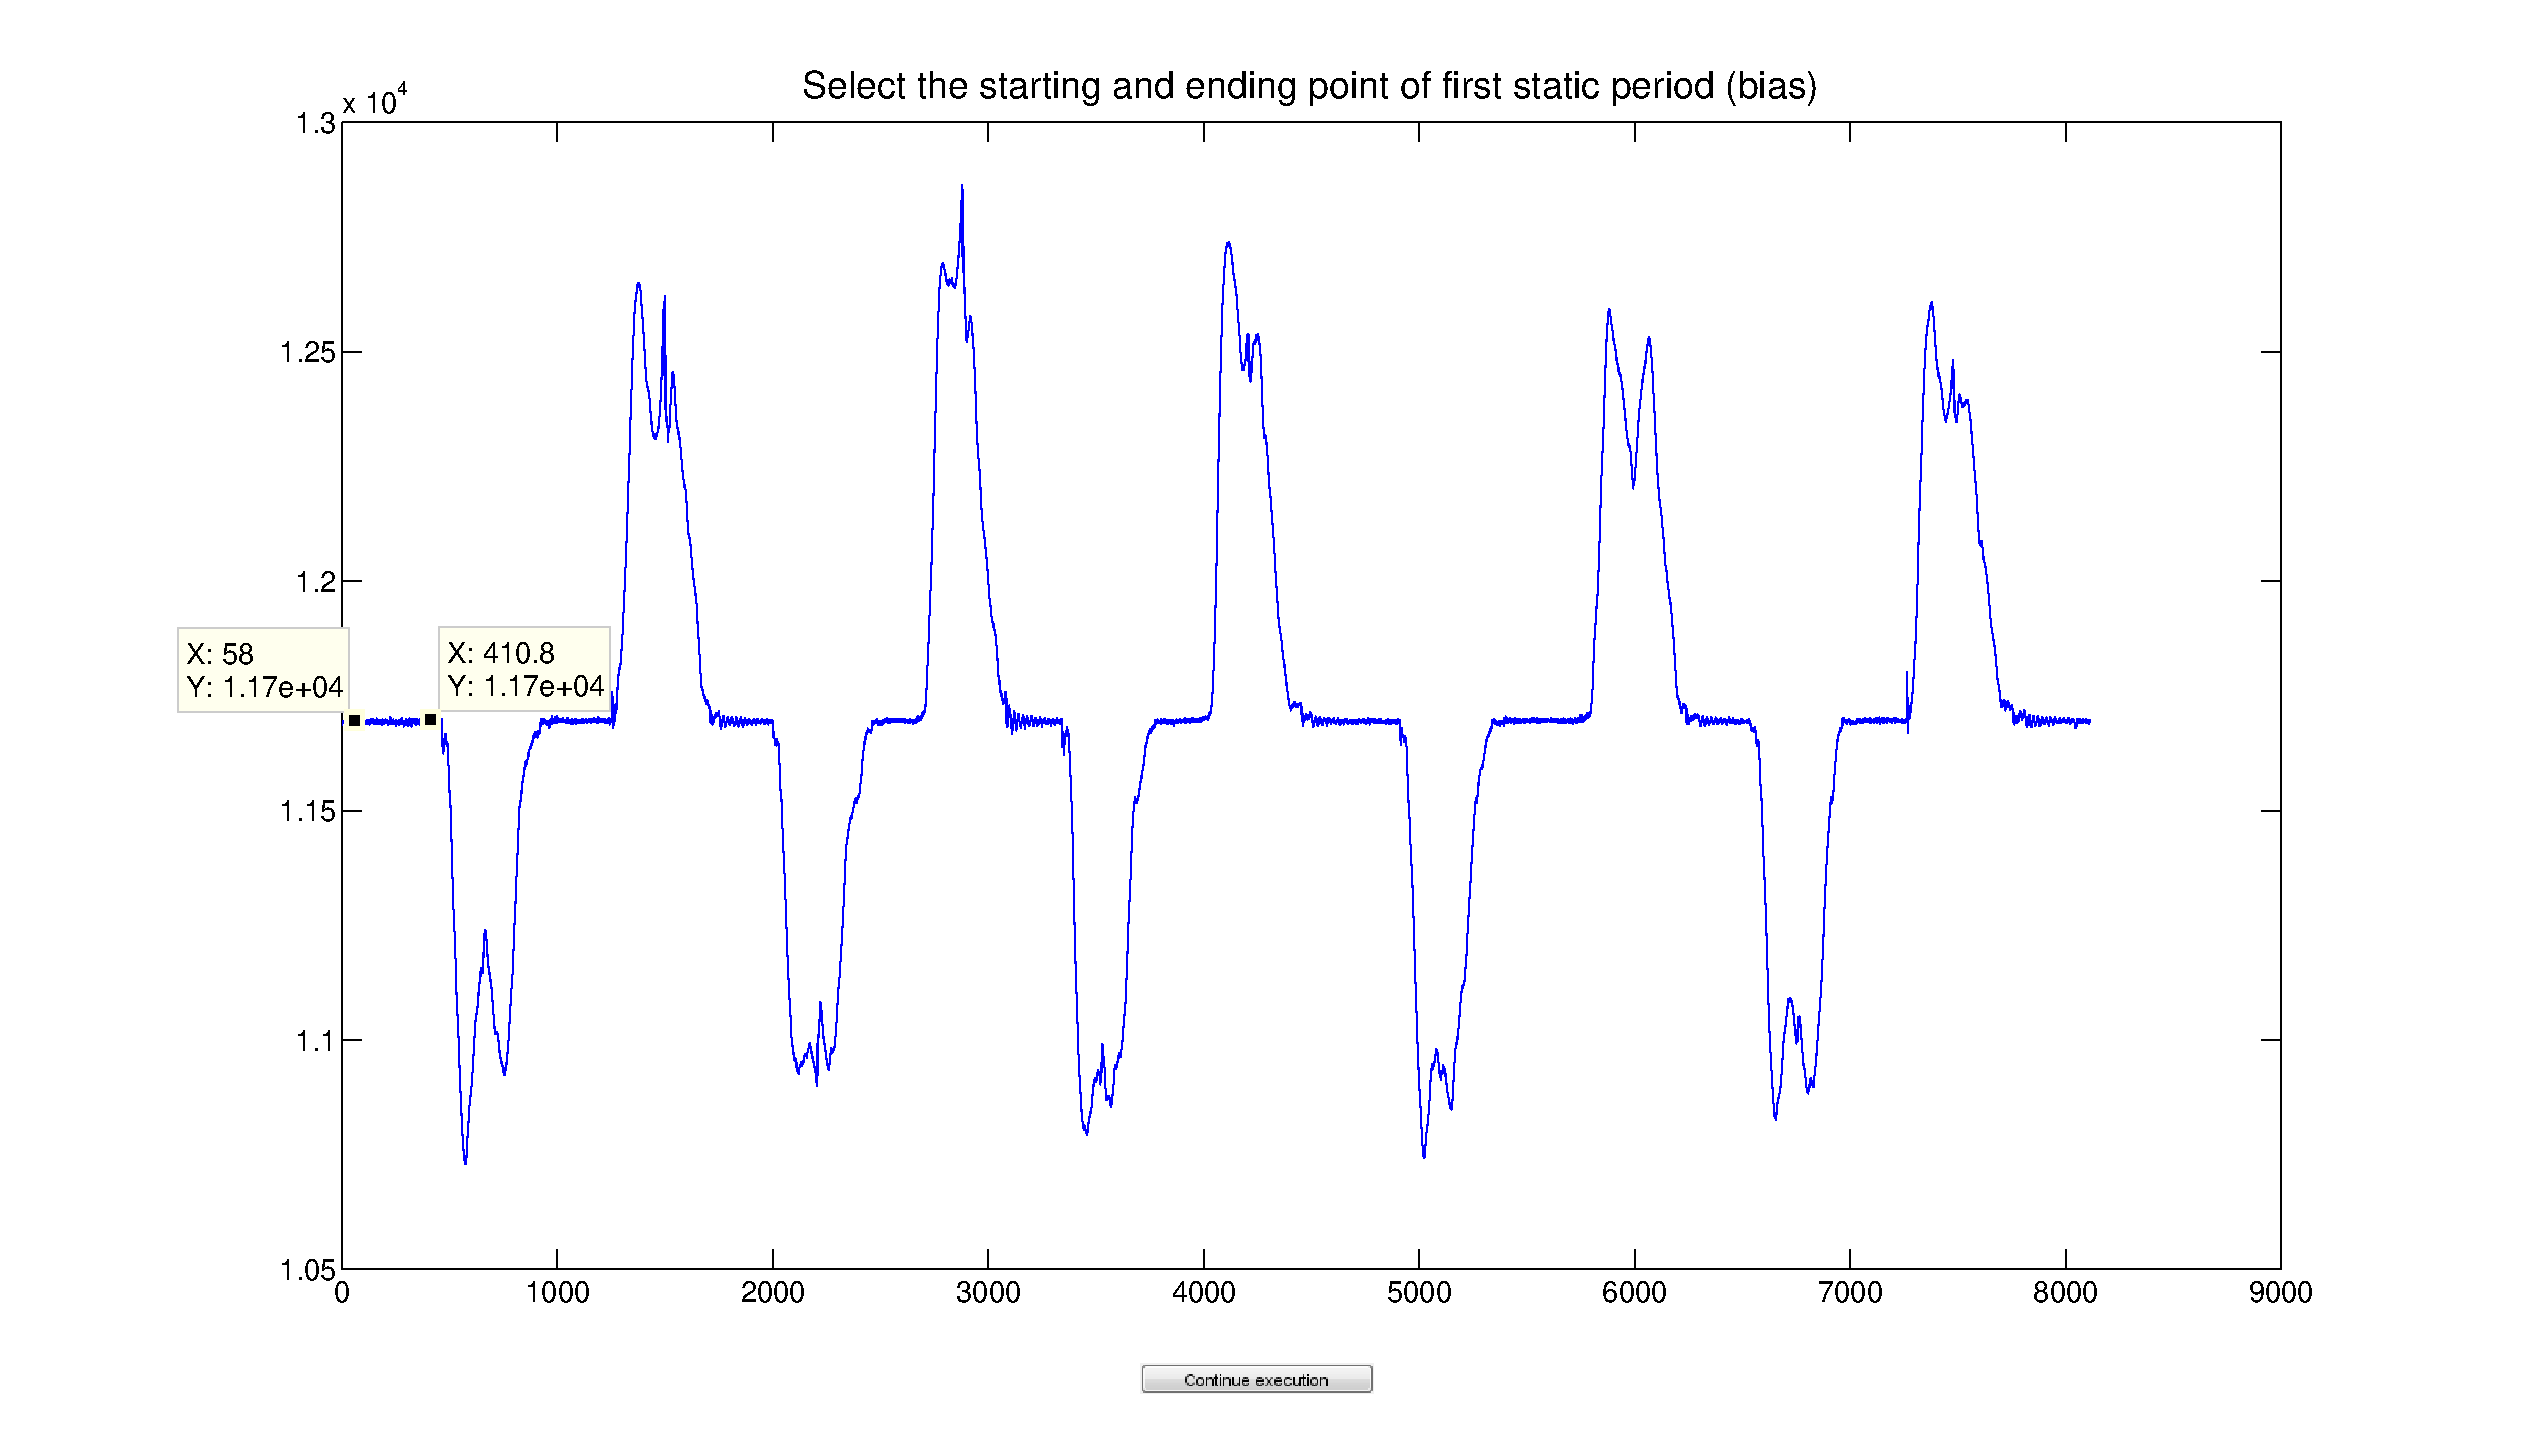
\includegraphics[width=1\textwidth]{figures/gyro_cal_routine_bias.eps}
\caption{Gyroscope calibration routine: selection of static period to compute bias.}
\label{fig:gyro_cal_routine_bias}
\end{figure}

\begin{figure}[H]
\centering
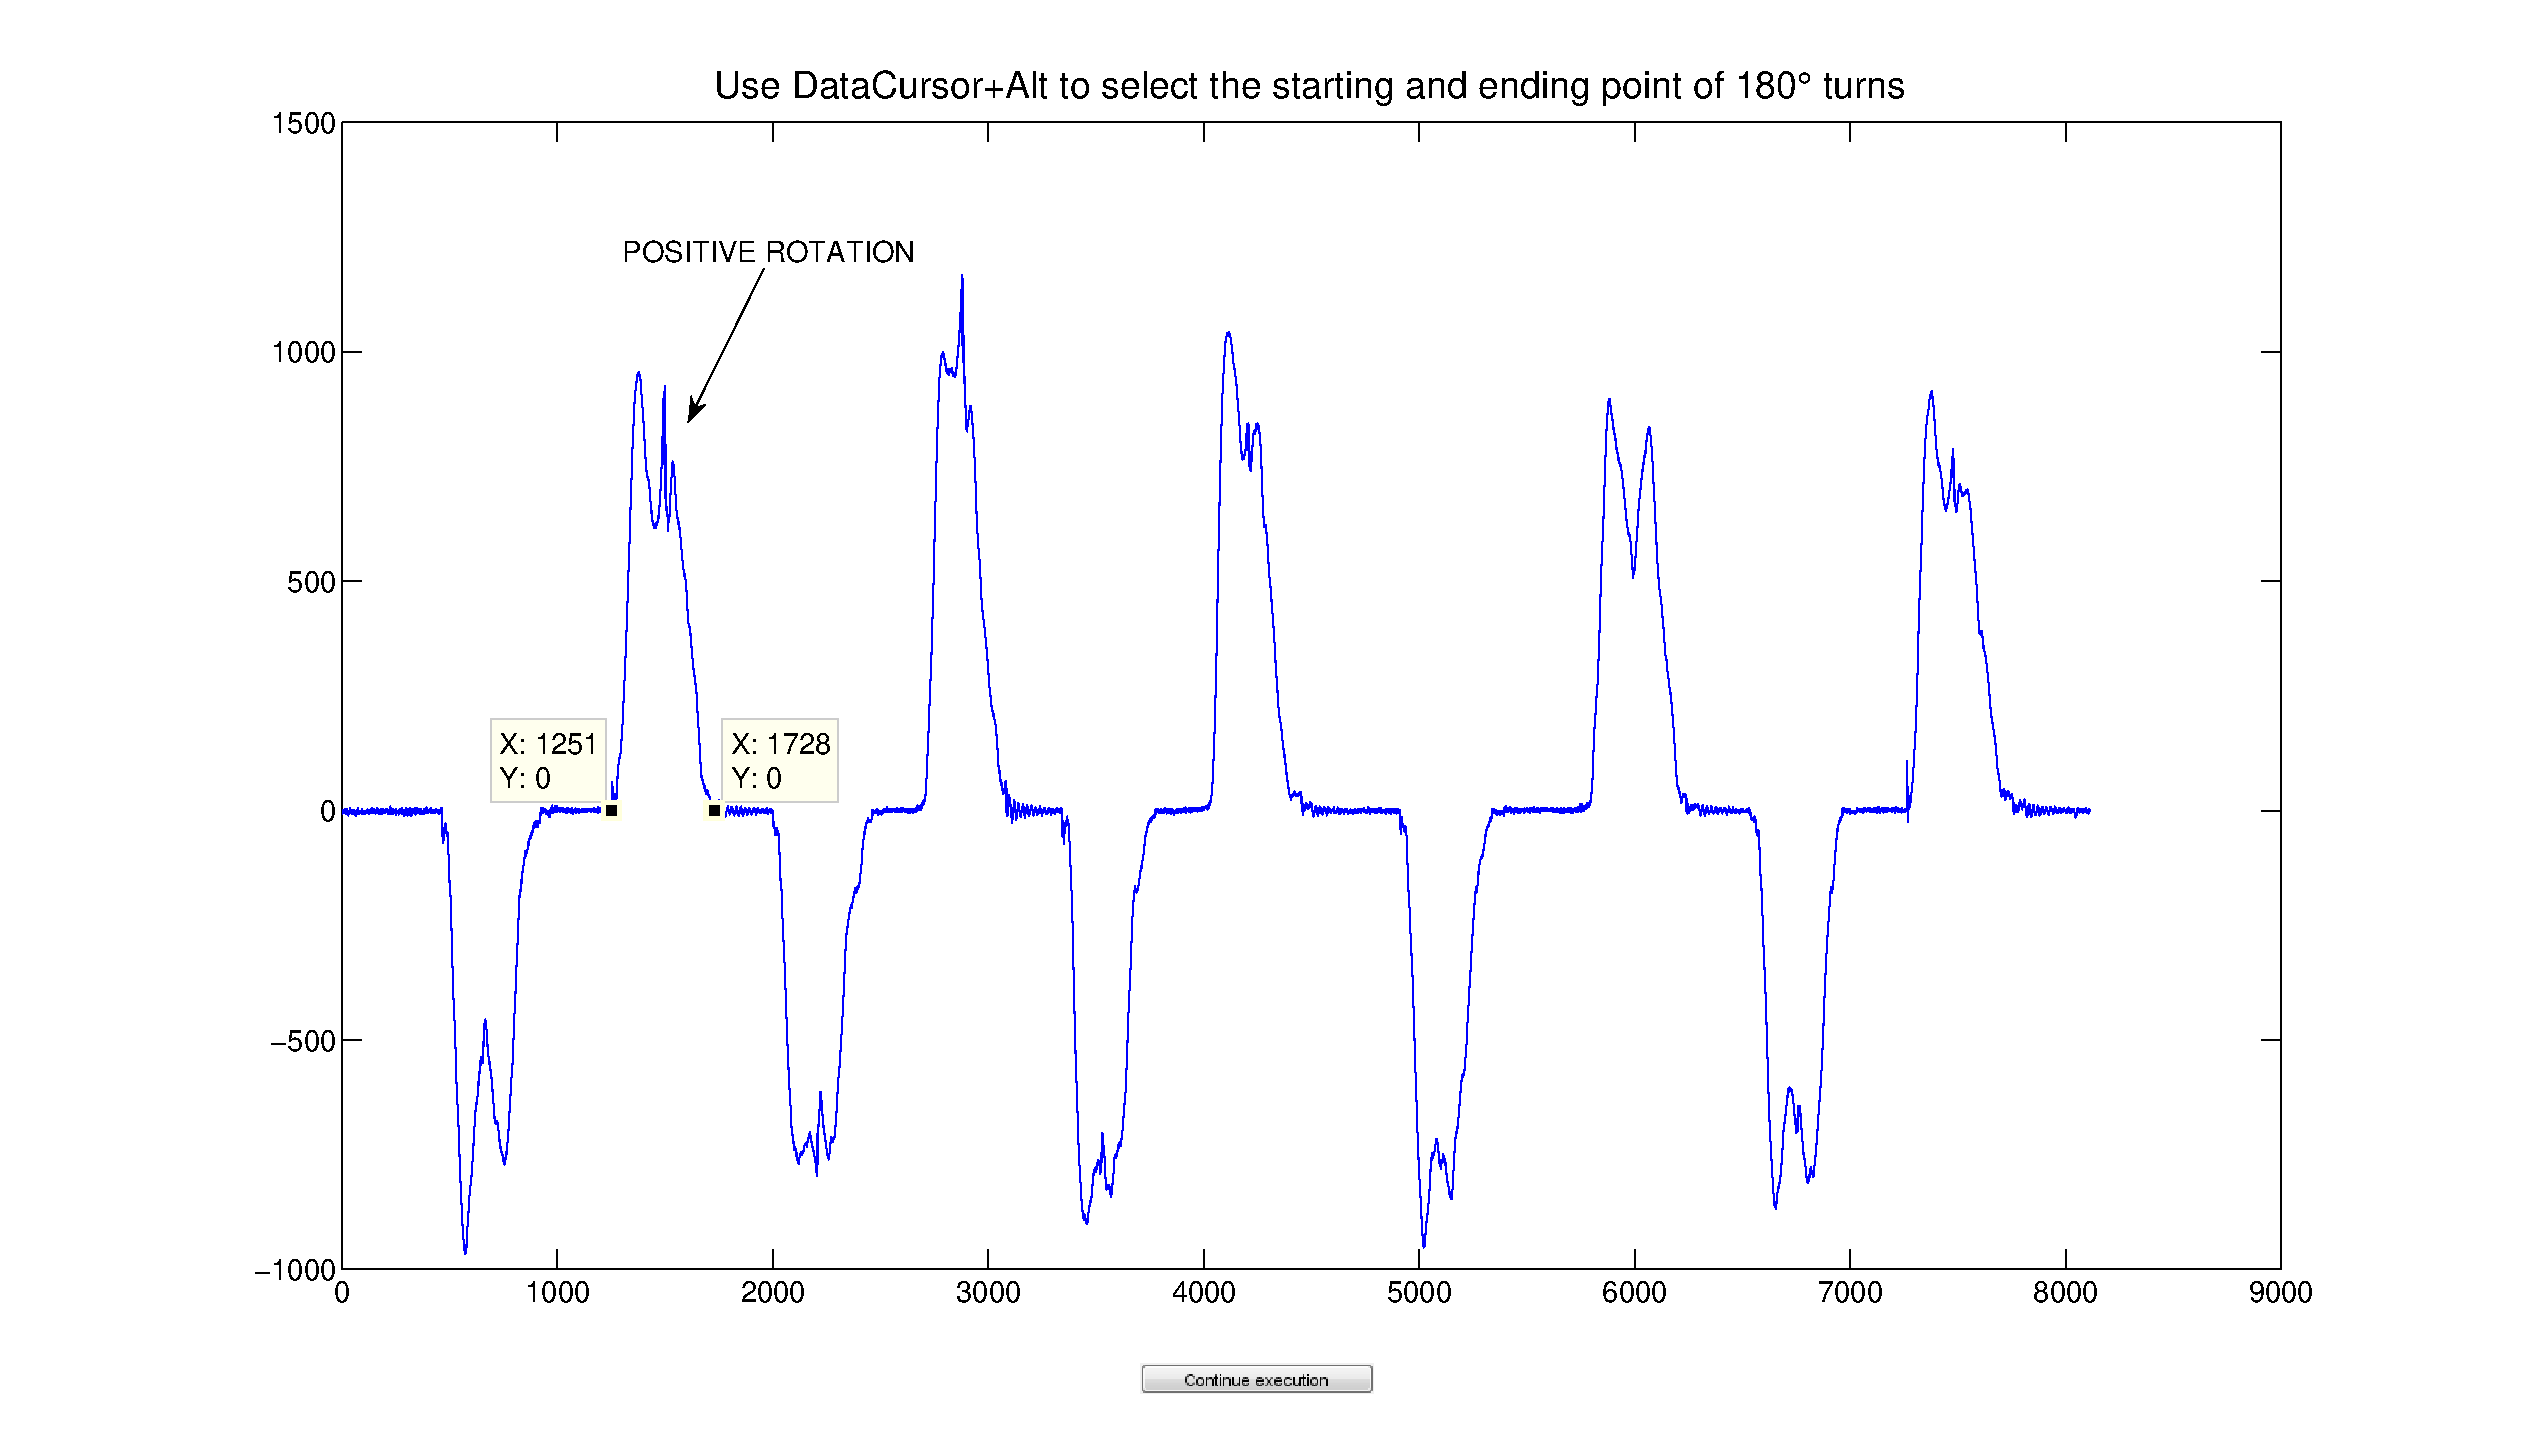
\includegraphics[width=1\textwidth]{figures/gyro_cal_routine_sf.eps}
\caption{Gyroscope calibration routine: selection of positive rotations to compute scale factor.}
\label{fig:gyro_cal_routine_sf}
\end{figure}

Table \ref{tab:gyro_cal_params} lists the computed calibration parameters for all GaitWatch's gyroscopes.

\begin{table}[H]\footnotesize
\caption{Calibration parameters of gyroscopes (valid as of December the 10th, 2013).}
	\centering
		\begin{tabular}{|c|c|c|c|}\hline
		\label{tab:gyro_cal_params}
		Unit				& Axis 	& Scale factor 	& Bias 	\\ \hline
		Left shank 	& Y			& -5.84					& 11591 \\
		Left thigh	& Y			& -6.36					& 11720 \\
		Right shank & Y			& -5.95					& 11618 \\
		Right thigh & Y			& -6.40					& 11740 \\ 
		Left arm	  & X			& -5.89					& 12087 \\
		Left arm		& Y			& 5.75					& 10937 \\
		Right arm   & X			& -6.02					& 11543 \\
		Right arm   & Y			& 5.64					& 11415 \\ 
		Trunk				& X			& -16.15				& -10		\\
		Trunk				& Y			& 16.02					& 62		\\	
		Trunk				& Z			& 16.23					& 31		\\
		\hline
		\end{tabular}
\end{table}

\subsection{Wrap-up}
\label{subsec:cal_wrapup}
\indent \indent As a final summary, once all the calibration parameters from all the sensors are computed, we only need to apply the following equations,

\begin{itemize}
\item \textbf{Accelerometer}:
	\begin{itemize}
	\item \textit{Triaxial accelerometer}:
		\begin{equation}
		\label{eq:cal_acceleration_summary}
		\mathbf{a}_{cal}=S^{-1}(\mathbf{a}_{raw}-\mathbf{b})
		\end{equation}
	\item \textit{Biaxial accelerometer}:
		\begin{equation}
		\label{eq:acc_1D_cal_equation_summary}
		a_{cal} = k\cdot a_{raw} + b
		\end{equation}
	\end{itemize}
\item \textbf{Magnetometer}:
	\begin{equation}
	\label{eq:cal_mag_summary}
	\mathbf{h}_{cal}=S^{-1}(\mathbf{h}_{raw}-\mathbf{b})
	\end{equation}
\item \textbf{Gyroscope}:
\begin{equation}
\label{eq:gyro_cal2_summary}
\omega_{cal} = \frac{u_{raw}-b}{k} 
\end{equation}
\end{itemize}
	\clearemptydoublepage
  \chapter{Computation of Orientation}
\label{ch:orientationcomp}
\section{Computing the orientation using Euler Angles}
\subsection{Integration of angular rate}

\indent \indent Triaxial gyroscopes measure the angular rate around each one of the Cartesian axes relative to the body frame. Such angular rate can be integrated to estimate the rotation angle from time instants $t_{0}$ to $t_{1}$. Therefore, we can compute the position of the body relative to the navigation frame if, and only if, the initial orientation of the body frame with respect to the navigation frame is known. A straight forward solution is to use the approach based on the projection of the gravity and earth's magnetic field vectors to compute such initial orientation when the body is static.\\
\indent Many different numerical integration methods can be used to integrate the angular rate. In this case we will use the numerical integration based on the trapezoidal rule which calculates the area under the function performing a trapezoidal approximation as follows:
\begin{gather}
\alpha(n)=\alpha_{0}+\frac{T}{2}\sum_{k=1}^{n}\left[\omega_{\mbox{\scriptsize g}}(k)+\omega_{\mbox{\scriptsize g}}(k-1)\right]
\label{eq:trapInt}
\end{gather}
Where T is the sample period, $n$ the sample number, $\omega_{\mbox{\scriptsize g}}(n)$ the gyro measurement at instant $n$ and $\alpha_{0}$ the angle at $n=0$. The angle can also be computed in a recursive way using
\begin{equation}
\alpha(n)=\alpha(n-1)+\frac{\mbox{T}}{2}\left[\omega_{\mbox{\scriptsize g}}(n)+\omega_{\mbox{\scriptsize g}}(n-1)\right]
\label{eq:trapIntRec}
\end{equation}
where $\alpha(0)=\alpha_{0}$.\\
\indent The main advantage of this method is that, once the initial orientation is known, it can be used either under low or high intensity motion conditions as the gyroscope measurements are not affected by linear acceleration. However, integration of noise and dynamic bias leads to a quick time growing offset which disrupts the computed angle. The effects of such integration are so devastating that the orientation estimate is absolutely erroneous after a few seconds as it can be seen in figure \ref{fig:dynBiasEff}).\\
\indent This method is, itself, unfeasible if not fused with the accelerometer and magnetometer approach. 
\begin{figure}
\centering
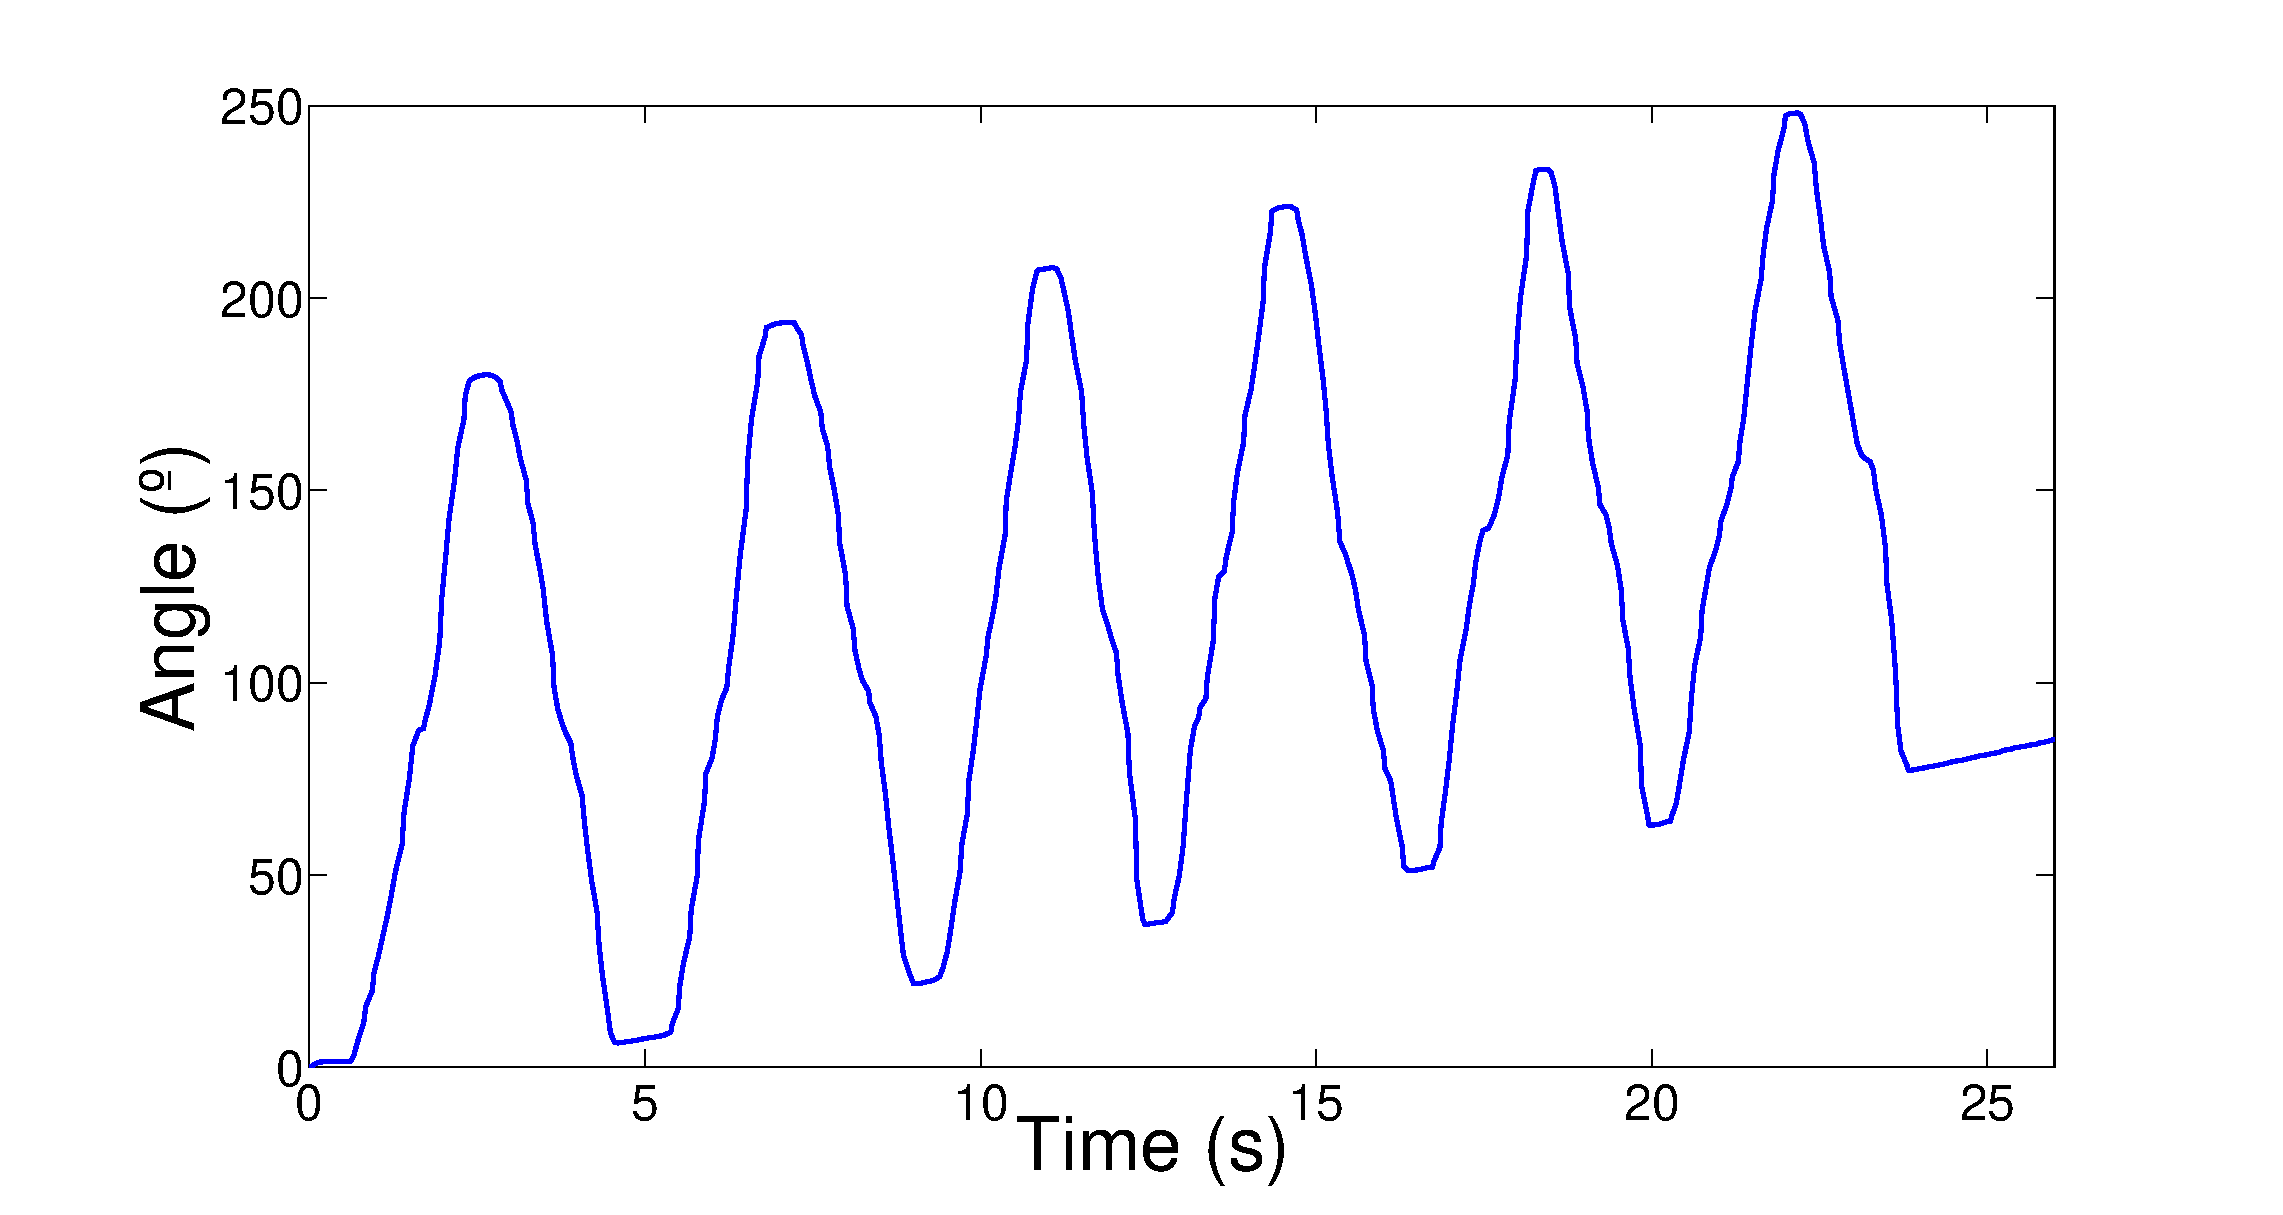
\includegraphics[width=0.7\textwidth]{figures/dynBiasEff.eps}
\caption{Effects of dynamic bias on the integrated gyroscope output signal.}
\label{fig:dynBiasEff}
\end{figure}


\subsection{Decomposition of gravity}
\indent We can use the projection of the Earth's gravity vector on the accelerometer's axes to estimate the orientation angle of the body frame with respect to the reference frame. In our case, this approach is used to compute the orientation angle of the thighs and shanks. Since only a biaxial accelerometer is available in the IMUs placed on these segments, we can only compute one of the two orientation angles (roll and pitch) which can be computed by means of this technique. We are interested on the angle of the segments defined in the XZ plane, that is, the angle around Y axis, which is defined as the pitch angle. The computation of the pitch will only be valid if the roll angle of the legs is close to zero. Since the legs move in the sagittal plane during gait, we can consider that the following expression will be valid to compute the pitch angle,

\begin{equation}
\label{eq:pitch_legs}
\theta_{k} = atan2(a_{z,k},a_{x,k})
\end{equation}

where $atan2$ is the quadrant-corrected arctangent function.

\subsection{Fusing the angular rate with the orientation angle observation computed with the accelerometer}
\subsubsection{The Kalman filter}
\label{subsubsec:kalman_filter}
\indent \indent The Kalman filter \cite{Kalman60}, \cite{Welch2001}, \cite{grewal_kalman_2008} is a set of mathematical equations that provides a means to estimate the state of a process minimizing the mean of the squared error. \\
\indent If we consider a time invariant linear continuous model:
\begin{gather}
\dot{\textbf{x}}(t)=\mbox{F}\textbf{x}(t)+\mbox{C}\textbf{u}(t)+\mbox{I}_{\mbox{\footnotesize n}}\textbf{w}(t)\\\nonumber
\textbf{z}(t)=\mbox{H}\textbf{x}(t)+\mbox{I}_{\mbox{\footnotesize q}}\textbf{v}(t)
\label{eq:contSystem}
\end{gather}
where,
\begin{itemize}
\item the operator $\dot{\mathbf{x}}$ denotes the first derivative of $\mathbf{x}$.
\item $\mathbf{x}(t)\in\mathbb{R}^{\mbox{\scriptsize n}}$ is the (n$\times$1) state vector including the n state variables that describe the system.
\item $\mathbf{z}(t)\in\mathbb{R}^{\mbox{\scriptsize q}}$ is the (q$\times$1) output vector including the q real observations (measurements) of the state variables of the process.
\item $\mathbf{u}(t)\in\mathbb{R}^{\mbox{\scriptsize p}}$ is the (p$\times$1) control vector including the p input control signals.
\item F is the (n$\times$n) state transition matrix, or simply the state matrix.
\item C is the (n$\times$p) input matrix.
\item H is the (q$\times$n) output matrix.
\item $\mbox{I}_{\mbox{\footnotesize n}}$ is the (n$\times$n) identity matrix.
\item $\mbox{I}_{\mbox{\footnotesize q}}$ is the (q$\times$q) identity matrix.
\item $\mathbf{w}(t)\in\mathbb{R}^{\mbox{\scriptsize n}}$ is the (n$\times$1) process noise vector.
\item $\mathbf{v}(t)\in\mathbb{R}^{\mbox{\scriptsize q}}$ is the (q$\times$1) observation noise vector.
\end{itemize}
In the absence of a control input we have:
\begin{gather}
\dot{\textbf{x}}(t)=\mbox{F}\textbf{x}(t)+\mbox{I}_{\mbox{\footnotesize n}}\textbf{w}(t)\\\nonumber
\textbf{z}(t)=\mbox{H}\textbf{x}(t)+\mbox{I}_{\mbox{\footnotesize q}}\textbf{v}(t)
\label{eq:contSystem2}
\end{gather}
If we apply the forward-Euler approximation:
\begin{equation}
\dot{x}(t)\simeq \frac{x(t+\mbox{dt})-x(t)}{\mbox{dt}}
\end{equation}
we get:
\begin{gather}
\frac{\textbf{x}(t+\mbox{dt})-\textbf{x}(t)}{\mbox{dt}}\simeq \mbox{F}\textbf{x}(t)+\mbox{I}_{\mbox{\footnotesize n}}\textbf{w}(t)\\\nonumber
\textbf{x}(t+\mbox{dt})\simeq \left[\mbox{F}\textbf{x}(t)+\mbox{I}_{\mbox{\footnotesize n}}\textbf{w}(t)\right]\mbox{dt}+\textbf{x}(t)\\\nonumber
\textbf{x}(t+\mbox{dt})\simeq \mbox{F}\textbf{x}(t)\mbox{dt}+\mbox{I}_{\mbox{\footnotesize n}}\textbf{w}(t)\mbox{dt}+\textbf{x}(t)\\\nonumber
\textbf{x}(t+\mbox{dt})\simeq \left[\mbox{F}\mbox{dt}+\mbox{I}_{\mbox{\footnotesize n}}\right]\textbf{x}(t)+\mbox{I}_{\mbox{\footnotesize n}}\textbf{w}(t)\mbox{dt}
\end{gather}
If we now discretize the model:
\begin{gather}
\textbf{x}_{k+1}=\left[\mbox{F}\mbox{dt}+\mbox{I}_{\mbox{\footnotesize n}}\right]\textbf{x}_k+\mbox{I}_{\mbox{\footnotesize n}}\mbox{dt}\textbf{w}_k\\\nonumber
\textbf{x}_{k+1}=\Phi\textbf{x}_{k}+\mbox{I}_{\mbox{\footnotesize n}}\mbox{dt}\textbf{w}_{k}\\\nonumber
\textbf{z}_{k}=\mbox{H}\textbf{x}_{k}+\mbox{I}_{\mbox{\footnotesize q}}\mathbf{v}_{k}
\end{gather}
or how it is usually represented:
\begin{equation}
\textbf{x}_{k}=\Phi\textbf{x}_{k-1}+\mbox{B}\textbf{w}_{k-1}
\label{eq:DiscreteSystem}
\end{equation}
\begin{equation}
\textbf{z}_{k}=\mbox{H}\textbf{x}_{k}+\mbox{I}_{\mbox{\footnotesize q}}\mathbf{v}_{k}
\label{eq:DiscreteSystem2}
\end{equation}
where,
\begin{itemize}
\item $\mathbf{x}\in\mathbb{R}^{\mbox{\scriptsize n}}$ is again the (n$\times$1) state vector of the linear dynamic system.
\item $\mathbf{z}\in\mathbb{R}^{\mbox{\scriptsize q}}$ is again the (q$\times$1) vector of observations.
\item $\Phi$ is now the (n$\times$n) state transition matrix of the discrete linear dynamic system.
\item H is again the (q$\times$n) measurement sensitivity matrix defining the linear relationship between the state of the dynamic system and measurements that can be made.
\item $\mbox{B}=\mbox{I}_{\footnotesize \mbox{n}}\mbox{dt}$, where dt is the sampling period.
\item $\mathbf{w}\in\mathbb{R}^{\mbox{\scriptsize n}}$ is again the (n$\times$1) process noise vector.
\item $\mathbf{v}\in\mathbb{R}^{\mbox{\scriptsize q}}$ is again the (q$\times$1) observation noise vector.
\end{itemize}
\indent \indent So, when applied to discrete signals, the Kalman filter aims to solve the problem of trying to estimate the state $\mbox{\textbf{x}}\in\mathbb{R}^{n}$ of a discrete-time controlled process that is defined by the model in equations (\ref{eq:DiscreteSystem}) and (\ref{eq:DiscreteSystem2}). In addition, $\textbf{w}_{k}$ and $\textbf{v}_{k}$ are assumed to be independent of each other, white, and with normal probability distributions
\begin{equation}
p(\textbf{w})\thicksim N(0,\mbox{Q})
\label{eq:ProbDistW}
\end{equation}
\begin{equation}
p(\textbf{v})\thicksim N(0,\mbox{R})
\label{eq:ProbDistV}
\end{equation}
where, in turn, Q and R are the process noise covariance and measurement noise covariance matrices respectively and can be considered to be invariant in practice.\\
\indent When deriving the equations for the Kalman filter, the goal is to find an equation that computes an a posteriori (updated/corrected with the measurement) state estimate $\hat{\textbf{x}}_{k}$ as a linear combination of an a priori (predicted) estimate $\hat{\textbf{x}}_{k}^{-}$ and a weighted difference between an actual measurement $\textbf{z}_{k}$ and a measurement prediction $\mbox{H}\hat{\textbf{x}}_{k}^{-}$,
\begin{equation}
\hat{\textbf{x}}_{k}=\hat{\textbf{x}}_{k}^{-}+\mbox{K}_{k}(\textbf{z}_{k}-H\hat{\textbf{x}}_{k}^{-}).
\label{eq:KalProcEst}
\end{equation}
The difference in (\ref{eq:KalProcEst}) is known as the measurement innovation, or the residual. The residual indicates the discordance between the predicted measurement $\mbox{H}\hat{\textbf{x}}_{k}^{-}$ and the actual measurement $\textbf{z}_{k}$.\\
\indent The matrix $\mbox{K}_{k}$ in (\ref{eq:KalProcEst}) is known as the Kalman gain and is chosen to be the gain that will minimize the a posteriori error covariance. Another way to see the weighting by $\mbox{K}_{k}$ is that as the measurement error covariance gets close to zero, the actual measurement $\textbf{z}_{k}$ is trusted more, while the predicted measurement $\mbox{H}\hat{\textbf{x}}_{k}^{-}$ is trusted less. Analogously, as the a priori estimate error covariance approaches zero the actual measurement is trusted less, while the predicted measurement is trusted more.\\
\indent The Kalman filter estimates a process by using a form of feedback control: the filter estimates the process state at some time and then obtains feedback in the form of noisy measurements. As such, the equations for the Kalman filter are divided into two groups: time update equations and measurement update equations.\\
\indent The time update equations can also be thought of as prediction equations, while the measurement update equations can be thought of as correction equations. If we assume $\Phi$, H, Q and R to be constant, the time update equations are as follows:
\begin{equation}
\hat{\textbf{x}}_{k}^{-}=\Phi\hat{\textbf{x}}_{k-1}^{-}
\label{eq:prioriProcEst}
\end{equation}
\begin{equation}
\mbox{P}_{k}^{-}=\Phi \mbox{P}_{k-1}\Phi^{T}+\mbox{Q}
\label{eq:prioriCov}
\end{equation}
while the measurement update equations are
\begin{equation}
\mbox{K}_{k}=\mbox{P}_{k}^{-}\mbox{H}^{T}(\mbox{H}\mbox{P}_{k}^{-}\mbox{H}^{T}+\mbox{R})^{-1}
\label{eq:KalGain}
\end{equation}
\begin{equation}
\hat{\textbf{x}}_{k}=\hat{\textbf{x}}_{k}^{-}+\mbox{K}_{k}(\textbf{z}_{k}-\mbox{H}\hat{\textbf{x}}_{k}^{-})
\label{eq:postProcEst}
\end{equation}
\begin{equation}
\mbox{P}_{k}=(\mbox{I}-\mbox{K}_{k}\mbox{H})\mbox{P}_{k}^{-}
\label{eq:postCov}
\end{equation}
where $\mbox{P}_{k}^{-}$ and $\mbox{P}_{k}$ are the a priori and a posteriori estimate error covariance respectively and $\mbox{K}_{k}$ is a factor known as the Kalman Gain.\\
\indent Consequently in order to build a computational algorithm the following steps must be implemented:
\begin{itemize}
\item Known parameters.
    \begin{enumerate}
    \item $\Phi$:   State transition matrix.
    \item H:  Measurement matrix.
    \item Q:  Process noise covariance matrix.
    \item R:  Measurement noise covariance matrix.
    \end{enumerate}
\item Computations.
    \begin{enumerate}
    \item Compute $\mbox{P}_{k}^{-}$ by substituting $\mbox{P}_{k-1}$, $\Phi$ and Q in (\ref{eq:prioriCov}).
    \item Compute $\mbox{K}_{k}$ by substituting $\mbox{P}_{k}^{-}$, H and R in (\ref{eq:KalGain}).
    \item Compute $\mbox{P}_{k}$ by substituting $\mbox{K}_{k}$ and $\mbox{P}_{k}^{-}$ in (\ref{eq:postCov}).
    \item Compute successive values of $\hat{\textbf{x}}_{k}$ (which is the output of the filter) recursively using (\ref{eq:prioriProcEst}), (\ref{eq:postProcEst}) and the computed values of $\mbox{K}_{k}$. Start with the given initial estimates $\hat{\textbf{x}}_0$ and $\mbox{P}_{0}$.
    \end{enumerate}
\end{itemize}

\indent Figure \ref{fig:StandardKalmanDiagram} shows the flow diagram of the standard approach of the Kalman filter without sensor fusion.
\begin{figure}[H]
\centering
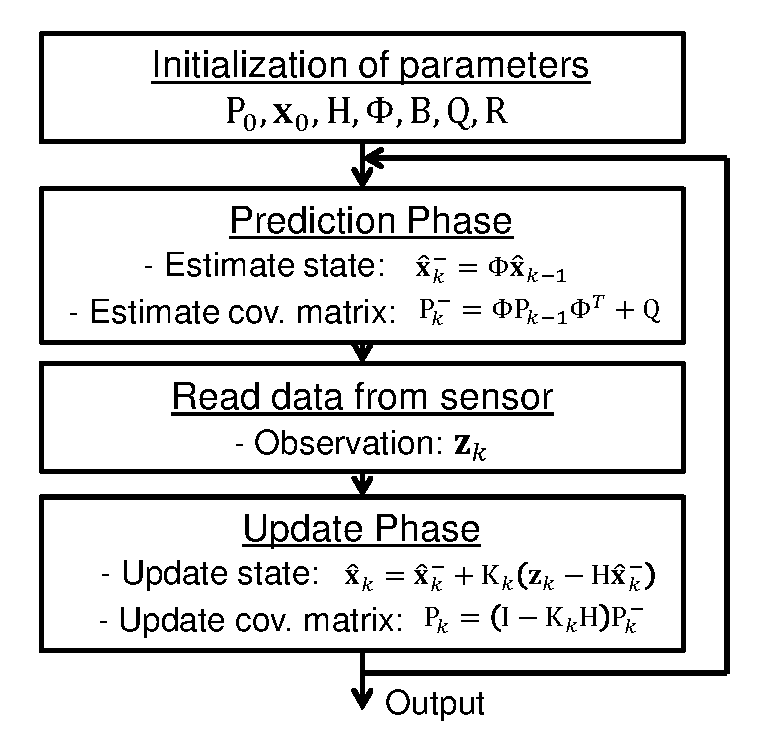
\includegraphics[width=0.6\textwidth]{figures/StandardKalmanDiagram.eps}
\caption{General diagram of the standard approach of the Kalman filter without sensor fusion.}
\label{fig:StandardKalmanDiagram}
\end{figure}

\subsubsection{The Kalman filter applied to orientation estimation}
\indent After this brief introduction to the basic theoretical fundamentals of the Kalman filter, we now explain how to employ it in a sensor fusion approach, and more specifically how to apply it to fuse the information coming from the two orientation estimation approaches explained to the moment.\\
\indent Let the state vector that we want to estimate be the following:
\begin{equation}
\mathbf{x}(t)=\left[
                \begin{array}{c}
                  \alpha(t) \\
                  \mbox{bias}(t) \\
                \end{array}
              \right]
\label{eq:kal_state}
\end{equation}
where $\alpha(t)$ is any of the orientation angles (roll, pitch or yaw), and bias(t) is the difference between the measured angular rate and the actual angular rate for $\alpha$.
\begin{equation}
\mbox{bias}(t)=\omega_{\mbox{\footnotesize meas}}(t)-\omega_{\mbox{\footnotesize actual}}(t)
\label{eq:kal_bias}
\end{equation}
Also, let $\mathbf{w}(t)=[w_{\alpha}(t)\;w_{bias}(t)]^{T}$, be the vector composed of the angle estimation noise and the angular rate bias noise respectively. The observation of the process, $\mathbf{z}(t)$ is the estimation of the angle computed using the accelerometer-magnetometer approach.
\begin{equation}
\mathbf{z}(t)=z(t)=\alpha(t)
\label{eq:Kal_fus_obs}
\end{equation}
We now proceed to obtain the expressions of the derivatives of the state variables:
\begin{equation}
\frac{\mbox{d}\alpha(t)}{\mbox{d}t}=\omega_{\mbox{\footnotesize actual}}(t)
\label{eq:Kal_fus_assum}
\end{equation}
knowing that $\omega_{\mbox{\footnotesize actual}}(t)=\omega_{\mbox{\footnotesize meas}}(t)-\mbox{bias}(t)$, i.e. the measured angular rate presents an offset with respect to its actual value:
\begin{equation}
\frac{\mbox{d}\alpha(t)}{\mbox{d}t}=\omega_{\mbox{\footnotesize meas}}(t)-\mbox{bias}(t)
\label{eq:Kal_fus_assum2}
\end{equation}
If we consider $\omega_{\mbox{\footnotesize meas}}(t)$ as a part of the process noise, $\omega_{\mbox{\footnotesize meas}}(t)=w_{\alpha}(t)$, we get:
\begin{equation}
\frac{\mbox{d}\alpha(t)}{\mbox{d}t}=-\mbox{bias}(t)+w_{\alpha}(t)
\label{eq:KalAngleDeriv}
\end{equation}
Thus, the first component of the process noise power, $w_{\alpha}(t)$ should be the variance of the angle signal computed with the accelerometer-magnetometer approach. \\ \\
\indent On the other hand, let the derivative of the second state variable, bias($t$), be the second component of the process noise:
\begin{equation}
\frac{\mbox{d}\mbox{bias}(t)}{\mbox{d}t}=w_{\mbox{\footnotesize bias}}(t)
\end{equation}
Then, the model of the system is as follows:
\begin{gather}
\mathbf{x}(t)=\left[
                \begin{array}{c}
                  \alpha(t) \\
                  \mbox{bias}(t) \\
                \end{array}
              \right];\nonumber\\
\frac{\mbox{d}\mathbf{x}(t)}{\mbox{d}t}=\frac{\mbox{d}}{\mbox{d}t}\left[
                                        \begin{array}{c}
                                          \alpha(t) \\
                                          \mbox{bias}(t) \\
                                        \end{array}
                                      \right]=\left[
                                                \begin{array}{cc}
                                                  0 & -1 \\
                                                  0 & 0 \\
                                                \end{array}
                                              \right]\left[
                                        \begin{array}{c}
                                          \alpha(t) \\
                                          \mbox{bias}(t) \\
                                        \end{array}
                                      \right]+\left[
                                                \begin{array}{cc}
                                                  1 & 0 \\
                                                  0 & 1 \\
                                                \end{array}
                                              \right]\left[
                                        \begin{array}{c}
                                          w_{\alpha}(t) \\
                                          w_{\mbox{\footnotesize bias}}(t) \\
                                        \end{array}
                                      \right];\nonumber\\
z(t)=\left[1\;0\right]\left[
                    \begin{array}{c}
                      \alpha(t) \\
                      \mbox{bias}(t) \\
                    \end{array}
                  \right]+v(t)
\label{eq:Kal_fus_System}
\end{gather}
If we now apply the approximations to discretize the system we get:
\begin{gather}
\mathbf{x}_{k+1}=\left[
                   \begin{array}{c}
                     \alpha_{k+1} \\
                     \mbox{bias}_{k+1} \\
                   \end{array}
                 \right]=\left[\left[
                           \begin{array}{cc}
                             1 & 0 \\
                             0 & 1 \\
                           \end{array}
                         \right]+\left[
                                  \begin{array}{cc}
                                    0 & \mbox{-dt} \\
                                    0 & 0 \\
                                   \end{array}\right]\right]\left[
                   \begin{array}{c}
                     \alpha_{k} \\
                     \mbox{bias}_{k} \\
                   \end{array}
                 \right]+\left[
                           \begin{array}{cc}
                             \mbox{dt} & 0 \\
                             0 & \mbox{dt} \\
                           \end{array}
                         \right]\left[
                   \begin{array}{c}
                     w_{\alpha,k} \\
                     w_{\mbox{\footnotesize bias},k} \\
                   \end{array}
                 \right];\nonumber\\
\mathbf{z}_{k+1}=\left[1\;0\right]\left[
                   \begin{array}{c}
                     \alpha_{k+1} \\
                     \mbox{bias}_{k+1} \\
                   \end{array}
                 \right]+v_{k+1}
\label{eq:Kal_fus_disc_system}
\end{gather}
or, equivalently:
\begin{gather}
\mathbf{x}_{k}=\left[
                   \begin{array}{c}
                     \alpha_{k} \\
                     \mbox{bias}_{k} \\
                   \end{array}
                 \right]=\left[
                           \begin{array}{cc}
                             1 & -\mbox{dt} \\
                             0 & 1 \\
                           \end{array}
                         \right]\left[
                   \begin{array}{c}
                     \alpha_{k-1} \\
                     \mbox{bias}_{k-1} \\
                   \end{array}
                 \right]+\left[
                           \begin{array}{cc}
                             \mbox{dt} & 0 \\
                             0 & \mbox{dt} \\
                           \end{array}
                         \right]\left[
                   \begin{array}{c}
                     w_{\alpha,k-1} \\
                     w_{\mbox{\footnotesize bias},k-1} \\
                   \end{array}
                 \right];\nonumber\\
\mathbf{z}_{k}=\left[1\;0\right]\left[
                   \begin{array}{c}
                     \alpha_{k} \\
                     \mbox{bias}_{k} \\
                   \end{array}
                 \right]+v_{k}
\label{eq:Kal_fus_disc_system2}
\end{gather}
Then, identifying terms, we have:
\begin{equation}
\Phi=\left[
       \begin{array}{cc}
         1 & -\mbox{dt} \\
         0 & 1 \\
       \end{array}
     \right],\quad \mbox{B}=\left[
                           \begin{array}{cc}
                             \mbox{dt} & 0 \\
                             0 & \mbox{dt} \\
                           \end{array}
                         \right],\quad \mbox{H}=\left[1\;0\right]
\label{eq:identified_filter_matrices}
\end{equation}

\indent Once we have defined the state equations of the discrete system, we repeat the equations of the Kalman filter and their order of application for the sake of clarity:
\begin{center}
\underline{PREDICTION EQUATIONS}
\end{center}
\vspace{-0.5cm}
\begin{equation}
\mathbf{\hat{x}}_{k}^{-}=\Phi\mathbf{\hat{x}}_{k-1}
\label{eq:Kal_fus_pred1}
\end{equation}
\begin{equation}
\mbox{P}_{k}^{-}=\Phi\mbox{P}_{k-1}\Phi^{T}+\mbox{Q}
\label{eq:Kal_fus_pred2}
\end{equation}
\begin{center}
\underline{UPDATE EQUATIONS}
\end{center}
\vspace{-0.5cm}
\begin{equation}
\mbox{K}_{k}=\frac{\mbox{P}_{k}^{-}\mbox{H}^{T}}{\mbox{H}\mbox{P}_{k}^{-}\mbox{H}^{T}+\mbox{R}}
\label{eq:Kalman_gain_update_phase}
\end{equation}
\begin{equation}
\mathbf{\hat{x}}_{k}=\mathbf{\hat{x}}_{k}^{-}+\mbox{K}_{k}(\mbox{z}_{k}-\mbox{H}\mathbf{\hat{x}}_{k}^{-})
\label{eq:state_vector_update_phase}
\end{equation}
\begin{equation}
\mbox{P}_{k}=(\mbox{I}-\mbox{K}_{k}\mbox{H})\mbox{P}_{k}^{-}
\label{eq:covariance_matrix_update_phase}
\end{equation}
where
\begin{itemize}
\item $\mathbf{\hat{x}}_{k}^{-}$ is the a priori state estimate.
\item $\mbox{P}_{k}^{-}$ is the a priori system covariance matrix.
\item $\mbox{Q}$ is the process noise covariance matrix and is defined as
\begin{equation}
\mbox{Q}=\left[
    \begin{array}{cc}
      \sigma_{\alpha} & 0 \\
      0 & \sigma_{\omega} \\
    \end{array}
  \right]
\label{eq:Kal_fus_proc_noise_cov_matrix}
\end{equation}
where $\sigma_{\alpha}$ is the variance of the angle computed with the acce\-le\-ro\-me\-ter-mag\-ne\-to\-me\-ter approach and $\sigma_{\omega}$ the variance of the angular rate measured by the gyroscope.
\item R, which in this case is a scalar, is the power of the observation noise and is defined as the variance of the accelerometer-magnetometer angle estimation ($\sigma_{\alpha}$).
\item $\mbox{K}_{k}$ is the Kalman filter gain.
\item $\mathbf{\hat{x}}_{k}$ is the a posteriori state estimate.
\item $\mbox{P}_{k}$ is the a posteriori system covariance matrix.
\end{itemize}
The reader may be wondering where exactly in the equations we have used the measured angular rate. Truth is that equations (\ref{eq:Kal_fus_pred1})-(\ref{eq:covariance_matrix_update_phase}) do not yet implement a sensor fusion approach as we are only using data coming from the accelerometer-magnetometer. The key of inserting sensor fusion to the system defined by these equations is to change the computation of the a priori prediction of the states $\mathbf{\hat{x}}_{k}^{-}$ as follows:
\begin{equation}
\mathbf{\hat{x}}_{k}^{-}=\left[
                           \begin{array}{c}
                             \alpha_{k}^{-} \\
                             \mbox{bias}_{k}^{-} \\
                           \end{array}
                         \right]=
\left[
                           \begin{array}{c}
                             \alpha_{k-1}+\left(\omega_{\mbox{\footnotesize meas},k}-\mbox{bias}_{k-1}\right)\mbox{dt} \\
                             \mbox{bias}_{k-1}\\
                           \end{array}
                         \right]
\label{eq:Kal_fus_real_system}
\end{equation}
This way, the a priori state estimate is being computed using information from both accelerometer-magnetometer and angular rate approaches.\\
\indent To end the explanation of the classical approach of the Kalman filter applied to fuse the information of the accelerometer-magnetometer and gyroscope, we include below the step by step operations that need to be carried
out by the complete algorithm:
\begin{enumerate}
\item Initialize the covariance matrix as a $2\times2$ identity matrix, $\mbox{P}=\mbox{I}_{2\times2}$.
\item Define the covariance matrix using equation (\ref{eq:Kal_fus_proc_noise_cov_matrix}). This matrix remains constant during the execution of the algorithm.
\item Define the measurement noise variance, $R$, which in this case is the variance of the accelerometer-magnetometer angle estimations, $R=\sigma_{\alpha}$. This value remains constant during the execution of the algorithm.
\item Define the state transition and the measurement matrices, $\Phi$ and H using equation (\ref{eq:identified_filter_matrices}).
\item Read data from accelerometer ($\mathbf{a}_{k}$), gyroscope ($\mathbf{\omega}_{k}$) and magnetometer ($\mathbf{h}_{k}$). \label{en:read_data}
\item Using $\textbf{a}_{k}$ and $\mathbf{h}_{k}$, compute the accelerometer-magnetometer angle estimation, $\alpha_{k}$, by applying any of the non-fusion orientation estimation methods explained within the previous subsections.
\item Compute the a priori estimation of the state vector using equation (\ref{eq:Kal_fus_real_system}).
\item Compute the a priori system covariance matrix using equation (\ref{eq:Kal_fus_pred2}).
\item Compute the Kalman gain using equation (\ref{eq:Kalman_gain_update_phase}), where $z_{k}=\alpha_{k}$.
\item Update the state vector using equation (\ref{eq:state_vector_update_phase}).
\item Update the system covariance matrix using equation (\ref{eq:covariance_matrix_update_phase}).
\item Return to step \ref{en:read_data}.
\end{enumerate}
\indent Figure \ref{fig:KalmanDiagramFusion} shows the flow diagram of the standard approach of the Kalman filter with sensor fusion.
\begin{figure}[H]
\centering
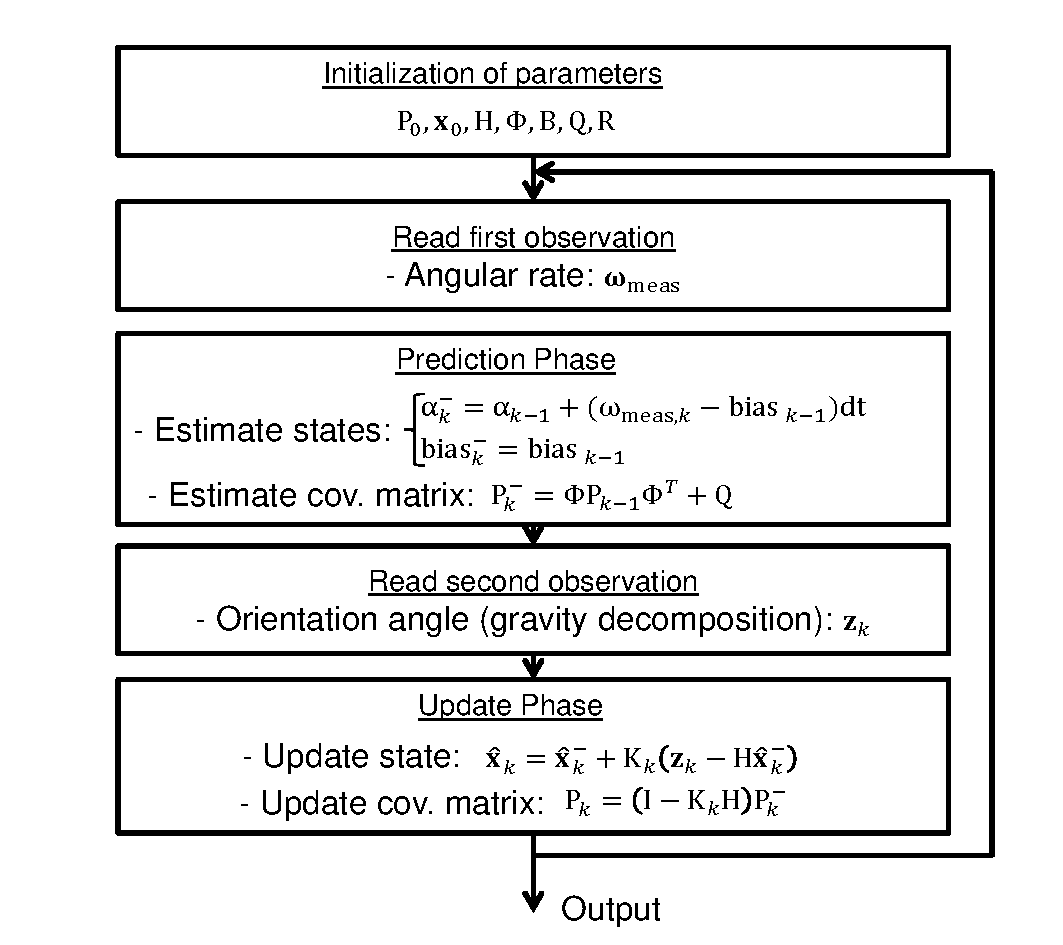
\includegraphics[width=0.8\textwidth]{figures/kalman_orientation_diag}
\caption{General diagram of the standard approach of the Kalman filter with sensor fusion.}
\label{fig:KalmanDiagramFusion}
\end{figure}

\section{Quaternion-based orientation determination}
\subsection{Using angular rate to compute orientation}
A way to compute the rate of change of the orientation of the Earth frame relative to the sensor frame is to compute the quaternion derivative $^{S}_{E}\dot{\textbf{q}}$, which is defined as follows,
\begin{equation}
\label{eq:quat_deriv}
^{S}_{E}\dot{\mathbf{q}} = \frac{1}{2}{^{S}_{E}\textbf{q}}\otimes{^{S}\boldsymbol{\omega}}
\end{equation}
where $^{S}_{E}\textbf{q}$ is the quaternion determining the orientation of the Earth frame relative to the sensor frame, $^{S}\boldsymbol{\omega} = \left[0\;\omega_{x}\;\omega_{y}\;\omega_{z}\right]$ is the measured angular rate vector in the sensor frame in quaternion form, and $\otimes$ is the quaternion (or Hamiltonian) product. \\
\indent Therefore, we can compute the orientation of the Earth frame relative to the sensor frame (computed from the angular rate) at time t  $^{S}_{E}\textbf{q}_{\omega,t}$ by simply numerically integrating the quaternion derivative in equation (\ref{eq:quat_deriv}).

\begin{equation}
\label{eq:quat_integration}
^{S}_{E}\mathbf{q}_{\omega,t} = ^{S}_{E}\mathbf{\hat{q}}_{t-1} + ^{S}_{E}\dot{\mathbf{q}}_{w,t}\Delta t
\end{equation}

where $^{S}_{E}\mathbf{\hat{q}}_{t-1}$ is the orientation quaternion estimated in $t-1$ by applying a sensor fusion algorithm (this will be later explained), and $\Delta t$ is the sampling frequency. So, if we plug equation (\ref{eq:quat_deriv}) into (\ref{eq:quat_integration}), we get

\begin{equation}
\label{eq:state_equations}
\begin{gathered}
\begin{multlined}
^{S}_{E}\mathbf{q}_{\omega,t} = \left[\hat{q}_{1,t-1}\;\hat{q}_{2,t-1}\;\hat{q}_{3,t-1}\;\hat{q}_{4,t-1}\right] + \frac{1}{2}\Delta t\left[\hat{q}_{1,t-1}\;\hat{q}_{2,t-1}\;\hat{q}_{3,t-1}\;\hat{q}_{4,t-1} \right]\otimes\left[0\;\omega_{x}\;\omega_{y}\;\omega_{z}\right] =\\ \noindent
= \left[\hat{q}_{1,t-1}\;\hat{q}_{2,t-1}\;\hat{q}_{3,t-1}\;\hat{q}_{4,t-1}\right] + \frac{1}{2}\Delta t\biggl[\underbrace{-\hat{q}_{2,t-1}\omega_{x}-\hat{q}_{3,t-1}\omega_{y}-\hat{q}_{4,t-1}\omega_{z}}_{y_{1'}}\\
\underbrace{\hat{q}_{1,t-1}\omega_{x}+\hat{q}_{3,t-1}\omega_{z}-\hat{q}_{4,t-1}\omega_{y}}_{y_{2'}}\;\underbrace{\hat{q}_{1,t-1}\omega_{y}-\hat{q}_{2,t-1}\omega_{z}+\hat{q}_{4,t-1}\omega_{x}}_{y_{3'}}\;\\
\underbrace{\hat{q}_{1,t-1}\omega_{z}+\hat{q}_{2,t-1}\omega_{y}-\hat{q}_{3,t-1}\omega_{x}}_{y_{4'}}\biggr]
\end{multlined}
\end{gathered}
\end{equation}

\subsection{Using acceleration and magnetic field to compute orientation}
Another possible way to compute the orientation is by using the accelerometer and the magnetometer measurements. The accelerometer measures the magnitude and direction of the Earth's gravitational field in addition to linear acceleration. The magnetometer measures as well the magnitude and direction of the Earth's magnetic field together with local magnetic flux and field perturbations. \\
\indent If the body is moving with quasi-static motion and the environment is magnetically stable, we can assume that the accelerometer will only measure the gravity and the magnetometer will only measure Earth's magnetic field. We will assume this in the following.\\
\indent In order to obtain a complete 9-DOF orientation estimate we need to combine both the accelerometer and the magnetometer as the accelerometer is not able to measure the orientation around the Z axis as it is parallel to the gravitational field. In some applications it is only necessary to measure pitch and/or roll, so there is no need for a magnetometer. However, for a quaternion-based solution we need both sensors as it is a 9-DOF estimation.\\
\indent Therefore, to estimate the complete orientation we can formulate an optimization problem where an orientation of the sensor $^{S}_{E}\dot{\mathbf{q}}$, is that which aligns a predefined reference direction of the field in the Earth frame, $^{E}\mathbf{\hat{d}}$, with the measured direction of the field in the sensor frame, $^{S}\mathbf{\hat{s}}$, using the quaternion rotation operation 

\begin{equation}
\label{eq:quat_rot}
^{E}\mathbf{v} = ^{E}_{S}\hat{\mathbf{q}}\otimes^{S}\mathbf{v}\otimes^{E}_{S}\hat{\mathbf{q}}
\end{equation}

where $^{E}\mathbf{v}$ and $^{S}\mathbf{v}$ represent the vector $\mathbf{v}$ measured in the Earth frame and the sensor frame respectively, and $^{E}_{S}\hat{\mathbf{q}}$ is the quaternion representing the orientation of the sensor frame with respect to the Earth frame. \\
\indent Hence, $^{E}_{S}\hat{\mathbf{q}}$ can be found as the solution of 

\begin{equation}
\label{eq:quat_opt_problem}
\min_{^{E}_{S}\hat{\mathbf{q}}\in\mathbb{R}^{4}}f\left(^{E}_{S}\hat{\mathbf{q}},^{E}\hat{\mathbf{d}},^{S}\hat{\mathbf{s}}\right)
\end{equation}

where 

\begin{equation}
\label{eq:quat_opt_func}
f\left(^{E}_{S}\hat{\mathbf{q}},^{E}\hat{\mathbf{d}},^{S}\hat{\mathbf{s}}\right) = ^{E}_{S}\hat{\mathbf{q}}^{*}\otimes^{E}\hat{\mathbf{d}}\otimes^{E}_{S}\hat{\mathbf{q}}-^{S}\hat{\mathbf{s}}
\end{equation}

In this case, we will use the gradient descent algorithm to optimize the function. The orientation quaternion at instant k+1 is computed applying

\begin{equation}
\label{eq:quat_gradient}
^{E}_{S}\hat{\mathbf{q}}_{k+1} = ^{E}_{S}\hat{\mathbf{q}}_{k}-\mu\frac{\nabla f\left(^{E}_{S}\hat{\mathbf{q}},^{E}\hat{\mathbf{d}},^{S}\hat{\mathbf{s}}\right)}{\left\Vert\nabla f\left(^{E}_{S}\hat{\mathbf{q}},^{E}\hat{\mathbf{d}},^{S}\hat{\mathbf{s}}\right)\right\Vert}
\end{equation}

where 

\begin{equation}
\label{eq:quat_nabla}
\nabla f\left(^{E}_{S}\hat{\mathbf{q}},^{E}\hat{\mathbf{d}},^{S}\hat{\mathbf{s}}\right) = J^{T}\left(^{E}_{S}\hat{\mathbf{q}}_{k},^{E}\hat{\mathbf{d}}\right)f\left(^{E}_{S}\hat{\mathbf{q}},^{E}\hat{\mathbf{d}},^{S}\hat{\mathbf{s}}\right)
\end{equation}

Where, in turn,

\begin{equation}
\label{eq:quat_opt_func_extended}
^{E}_{S}\hat{\mathbf{q}}^{*}\otimes^{E}\hat{\mathbf{d}}\otimes^{E}_{S}\hat{\mathbf{q}}-^{S}\hat{\mathbf{s}} = 
\left[\begin{array}{c}
	2d_{x}\left(\frac{1}{2} - q_{3}^{2} - q_{4}^{2}\right) + 2d_{x} + 2d_{y}\left(q_{1}q_{4}+q_{2}q_{3}\right) +2d_{z}\left(q_{2}q_{4}-q_{1}q_{3}\right) - s_{x} \\
	2d_{x}\left(q_{2}q_{3} - q_{1}q_{4}\right) + 2d_{y}\left(\frac{1}{2} - q_{2}^2 - q_{4}^2\right) + 2d_{z}\left(q_{1}q_{2} + q_{3}q_{4}\right) - s_{y} \\
	2d_{x}\left(q_{1}q_{3} + q_{2}q_{4}\right) + 2d_{y}\left(q_{3}q_{4} - q_{1}q_{2}\right) + 2d_{z}\left(\frac{1}{2} - q_{2}^2 - q_{3}^2\right) - s_{z}
\end{array}\right]
\end{equation}

As we aforementioned,

\begin{itemize}
\item $^{E}_{S}\hat{\mathbf{q}} = \left[q_{1}\: q_{2}\: q_{3}\: q_{4}\right]\rightarrow$ Estimated orientation quaternion.
\item $^{E}\hat{\mathbf{d}} = \left[0\: d_{x}\: d_{y}\: d_{z}\right]\rightarrow$ Predefined reference direction of the field in the Earth frame.
\item $^{S}\hat{\mathbf{s}} = \left[0\: s_{x}\: s_{y}\: s_{z}\right]\rightarrow$ Measured direction of the field in the sensor frame.
\end{itemize}

In our case, we have two reference vectors, the Earth's gravitational and magnetic field vectors. Therefore, we will use both to have a complete 9DOF orientation estimation. We will start by deriving the equations for the Earth's gravitational field and the accelerometer. For this case, $^{E}\hat{\mathbf{d}} = ^{E}\hat{\mathbf{g}} = \left[0\: 0\: 0\: 1\right]$ and $^{S}\hat{\mathbf{s}} = ^{S}\hat{\mathbf{a}} = \left[0\: a_{x}\: a_{y}\: a_{z}\right]$. Then, equation (\ref{eq:quat_opt_func_extended}) is reduced to,

\begin{equation}
\label{eq:quat_opt_func_reduced}
f\left(^{E}_{S}\hat{\mathbf{q}},^{E}\hat{\mathbf{g}},^{S}\hat{\mathbf{a}}\right) = ^{E}_{S}\hat{\mathbf{q}}^{*}\otimes^{E}\hat{\mathbf{g}}\otimes^{E}_{S}\hat{\mathbf{q}}-^{S}\hat{\mathbf{a}} = \left[\begin{array}{c}
														 \underbrace{2\left(q_{2}q_{4} - q_{1}q_{3}\right) - a_{x}}_{F_{1}} \\
														 \underbrace{2\left(q_{1}q_{2} + q_{3}q_{4}\right) - a_{y}}_{F_{2}} \\
														 \underbrace{2\left(\frac{1}{2}-q_{2}^2-q_{3}^2\right) - a_{z}}_{F_{3}}
														\end{array}\right]
\end{equation}

As it was shown in equation (\ref{eq:quat_nabla}),

\begin{equation}
\label{eq:quat_nabla2}
\nabla f\left(^{E}_{S}\hat{\mathbf{q}},^{E}\hat{\mathbf{g}},^{S}\hat{\mathbf{a}}\right) = J^{T}\left(^{E}_{S}\hat{\mathbf{q}}_{k},^{E}\hat{\mathbf{g}}\right)f\left(^{E}_{S}\hat{\mathbf{q}},^{E}\hat{\mathbf{g}},^{S}\hat{\mathbf{a}}\right)
\end{equation}

Hence, we are only missing the computation of the Jacobian $J\left(^{E}_{S}\hat{\mathbf{q}}_{k},^{E}\hat{\mathbf{g}}\right)$, which is carried out by applying the following equation,

\begin{equation}
\label{eq:quat_jacobian}
J\left(^{E}_{S}\hat{\mathbf{q}}_{k},^{E}\hat{\mathbf{g}}\right) = \left[\begin{array}{cccc}
																																				\frac{\partial F_{1}}{\partial q_{1}} & \frac{\partial F_{1}}{\partial q_{2}} & \frac{\partial F_{1}}{\partial q_{3}} & \frac{\partial F_{1}}{\partial q_{4}} \\
																																				\frac{\partial F_{2}}{\partial q_{1}} & \frac{\partial F_{2}}{\partial q_{2}} & \frac{\partial F_{2}}{\partial q_{3}} & \frac{\partial F_{2}}{\partial q_{4}} \\
																																				\frac{\partial F_{3}}{\partial q_{1}} & \frac{\partial F_{3}}{\partial q_{2}} & \frac{\partial F_{3}}{\partial q_3{}} & \frac{\partial F_{3}}{\partial q_{4}}
																																			\end{array}\right] =
																																			\left[\begin{array}{cccc}
																																			-2q_{3} &  2q_{4} & -2q_{1} &  2q_{2} \\
																																			 2q_{2} &  2q_{1} &  2q_{4} &  2q_{3} \\
																																			      0 & -4q_{2} & -4q_{3} &       0
																																			\end{array}\right]
\end{equation}

We are now done with the accelerometer part, let's continue with the magnetometer which is going to provide the Yaw angle which can not be computed with the accelerometer. For the magnetometer, $^{E}\hat{\mathbf{d}} = ^{E}\hat{\mathbf{b}} = \left[0\: b_{x}\: 0\: b_{z}\right]$ and $^{S}\hat{\mathbf{s}} = ^{S}\hat{\mathbf{h}} = \left[0\: h_{x}\: h_{y}\: h_{z}\right]$.

\begin{equation}
\label{eq:quat_opt_func_reduced_mag}
f\left(^{E}_{S}\hat{\mathbf{q}},^{E}\hat{\mathbf{b}},^{S}\hat{\mathbf{h}}\right) = {^{E}_{S}\hat{\mathbf{q}}^{*}}\,\otimes\, {^{E}\hat{\mathbf{b}}}\,\otimes\, {^{E}_{S}\hat{\mathbf{q}}}-^{S}\hat{\mathbf{h}} = \left[\begin{array}{c}
														 \underbrace{2b_{x}\left(\frac{1}{2} - q_{3}^2-q_{4}^2\right) + 2b_{z}\left(q_{2}q_{4} - q_{1}q_{3}\right)- h_{x}}_{F_{4}} \\
														 \underbrace{2b_{x}\left(q_{2}q_{3} - q_{1}q_{4}\right) + 2b_{z}\left(q_{1}q_{2} + q_{3}q_{4}\right) - h_{y}}_{F_{5}} \\
														 \underbrace{2b_{x}\left(q_{1}q_{3} + q_{2}q_{4}\right) + 2b_{z}\left(\frac{1}{2} - q_{2}^2 - q_{3}^2\right)- h_{z}}_{F_{6}}
														\end{array}\right]
\end{equation}

Analogously as in equation (\ref{eq:quat_jacobian}),

\begin{equation}
\label{eq:quat_jacobian_mag}
\begin{gathered}
\begin{multlined}
J\left(^{E}_{S}\hat{\mathbf{q}}_{k},^{E}\hat{\mathbf{b}}\right) = \left[\begin{array}{cccc}
																																				\frac{\partial F_{4}}{\partial q_{1}} & \frac{\partial F_{4}}{\partial q_{2}} & \frac{\partial F_{4}}{\partial q_{3}} & \frac{\partial F_{4}}{\partial q_{4}} \\
																																				\frac{\partial F_{5}}{\partial q_{1}} & \frac{\partial F_{5}}{\partial q_{2}} & \frac{\partial F_{5}}{\partial q_{3}} & \frac{\partial F_{5}}{\partial q_{4}} \\
																																				\frac{\partial F_{6}}{\partial q_{1}} & \frac{\partial F_{6}}{\partial q_{2}} & \frac{\partial F_{6}}{\partial q_3{}} & \frac{\partial F_{6}}{\partial q_{4}}
																																			\end{array}\right] = \\
																																			= \left[\begin{array}{cccc}
																																			-2b_{z}q_{3} &  2b_{z}q_{4} & -2b_{z}q_{1} &  2b_{z}q_{2} \\
																																			-2b_{x}q_{4} + 2b_{z}q_{2} &  2b_{x}q_{3} + 2b_{z}q_{1} &  2b_{x}q_{2} + 2b_{z}q_{4} & -2b_{x}q_{1} + 2b_{z}q_{3} \\
																																			 2b_{x}q_{3} & 2b_{x}q_{4} - 4b_{z}q_{2} & 2b_{x}q_{1} - 4b_{z}q_{3} &  2b_{x}q_{2}
																																			\end{array}\right]
\end{multlined}
\end{gathered}
\end{equation}

So, finally, if we put everything together, these are the equations that need to be implemented to compute the orientation quaternion using accelerometer and magnetometer data,

\begin{gather}
\label{eq:quat_gradient_final}
^{E}_{S}\hat{\mathbf{q}}_{k+1} = {^{E}_{S}\hat{\mathbf{q}}_{k}}-\mu\frac{\nabla f\left(^{E}_{S}\hat{\mathbf{q}},^{E}\hat{\mathbf{gb}},^{S}\hat{\mathbf{ah}}\right)}{\left\Vert\nabla f\left(^{E}_{S}\hat{\mathbf{q}},^{E}\hat{\mathbf{gb}},^{S}\hat{\mathbf{ah}}\right)\right\Vert} \\
\nabla f\left(^{E}_{S}\hat{\mathbf{q}},^{E}\hat{\mathbf{gb}},^{S}\hat{\mathbf{ah}}\right) = J^{T}\left(^{E}_{S}\hat{\mathbf{q}}_{k},^{E}\hat{\mathbf{gb}}\right)f\left(^{E}_{S}\hat{\mathbf{q}},^{E}\hat{\mathbf{ah}},^{S}\hat{\mathbf{s}}\right) \\
\label{eq:quat_function_final}
f\left(^{E}_{S}\hat{\mathbf{q}},^{E}\hat{\mathbf{ah}},^{S}\hat{\mathbf{s}}\right) = \left[\begin{array}{c}
																																										 2\left(q_{2}q_{4} - q_{1}q_{3}\right) - a_{x} \\
																																										 2\left(q_{1}q_{2} + q_{3}q_{4}\right) - a_{y} \\
																																										 2\left(\frac{1}{2}-q_{2}^2-q_{3}^2\right) - a_{z} \\
																																										 2b_{x}\left(\frac{1}{2} - q_{3}^2-q_{4}^2\right) + 2b_{z}\left(q_{2}q_{4} - q_{1}q_{3}\right)- h_{x} \\
																																										 2b_{x}\left(q_{2}q_{3} - q_{1}q_{4}\right) + 2b_{z}\left(q_{1}q_{2} + q_{3}q_{4}\right) - h_{y} \\
																																										 2b_{x}\left(q_{1}q_{3} + q_{2}q_{4}\right) + 2b_{z}\left(\frac{1}{2} - q_{2}^2 - q_{3}^2\right)- h_{z}
																																										\end{array}\right] 
\end{gather}
\begin{gather}
\label{eq:final_Jacobian}
\begin{gathered}
\begin{multlined}																																							
J\left(^{E}_{S}\hat{\mathbf{q}}_{k},^{E}\hat{\mathbf{gb}}\right) = \left[\begin{array}{cccc}
																																				\frac{\partial F_{1}}{\partial q_{1}} & \frac{\partial F_{1}}{\partial q_{2}} & \frac{\partial F_{1}}{\partial q_{3}} & \frac{\partial F_{1}}{\partial q_{4}} \\
																																				\frac{\partial F_{2}}{\partial q_{1}} & \frac{\partial F_{2}}{\partial q_{2}} & \frac{\partial F_{2}}{\partial q_{3}} & \frac{\partial F_{2}}{\partial q_{4}} \\
																																				\frac{\partial F_{3}}{\partial q_{1}} & \frac{\partial F_{3}}{\partial q_{2}} & \frac{\partial F_{3}}{\partial q_3{}} & \frac{\partial F_{3}}{\partial q_{4}} \\
																																				\frac{\partial F_{4}}{\partial q_{1}} & \frac{\partial F_{4}}{\partial q_{2}} & \frac{\partial F_{4}}{\partial q_{3}} & \frac{\partial F_{4}}{\partial q_{4}} \\
																																				\frac{\partial F_{5}}{\partial q_{1}} & \frac{\partial F_{5}}{\partial q_{2}} & \frac{\partial F_{5}}{\partial q_{3}} & \frac{\partial F_{5}}{\partial q_{4}} \\
																																				\frac{\partial F_{6}}{\partial q_{1}} & \frac{\partial F_{6}}{\partial q_{2}} & \frac{\partial F_{6}}{\partial q_3{}} & \frac{\partial F_{6}}{\partial q_{4}}
																																			\end{array}\right] =\\ 
																																			 = \left[\begin{array}{cccc}
																																			-2q_{3} &  2q_{4} & -2q_{1} &  2q_{2} \\
																																			 2q_{2} &  2q_{1} &  2q_{4} &  2q_{3} \\
																																			      0 & -4q_{2} & -4q_{3} &       0 \\
																																			-2b_{z}q_{3} &  2b_{z}q_{4} & -2b_{z}q_{1} &  2b_{z}q_{2} \\
																																			-2b_{x}q_{4} + 2b_{z}q_{2} &  2b_{x}q_{3} + 2b_{z}q_{1} &  2b_{x}q_{2} + 2b_{z}q_{4} & -2b_{x}q_{1} + 2b_{z}q_{3} \\
																																			 2b_{x}q_{3} & 2b_{x}q_{4} - 4b_{z}q_{2} & 2b_{x}q_{1} - 4b_{z}q_{3} &  2b_{x}q_{2}
																																			\end{array}\right]
\end{multlined}
\end{gathered}
\end{gather}

The routine implementing the process above should be structured as follows for every instant $k$,

\begin{enumerate}[(i)]
\item Read the orientation quaternion for instant $k-1$, $^{E}_{S}\hat{\mathbf{q}}_{k-1}$.
\item Read the data from the accelerometer and the magnetometer for instant $k$. We then have $a_{x,k}\, a_{y,k}\, a_{z,k}\, h_{x,k}\, h_{y,k}$ and $h_{z,k}$.
\item Compute the Jacobian in equation (\ref{eq:final_Jacobian}) knowing that, 
	\begin{gather}
		\mathbf{m} = {^{E}_{S}\hat{\mathbf{q}}_{k-1}}\otimes \left[0\: h_{x,k}\: h_{y,k}\: h_{z,k}\right]\otimes {^{E}_{S}\hat{\mathbf{q}}_{k-1}^{*}} \\
		b_{x} = \sqrt{m_{2}^2+m_{3}^2} \\
		b_{z} = m_{4}
	\end{gather}
\item Compute the expression of $f\left(^{E}_{S}\hat{\mathbf{q}},^{E}\hat{\mathbf{ah}},^{S}\hat{\mathbf{s}}\right)$ in (\ref{eq:quat_function_final}).
\item Substitute the value of the expressions computed in the two previous steps in equation (\ref{eq:quat_gradient_final}) to compute the orientation quaternion for instant $k$, $^{E}_{S}\hat{\mathbf{q}}_{k}$.
\end{enumerate}

\subsection{Fusing the orientation quaternions computed with the angular rate and the acceleration and magnetic field}
\label{subsec:sensor_fusion}
\indent \indent In the previous two sections we have explained how to compute the orientation quaternion using two different approaches. The first one is based on the numerical integration of the angular rate. This approach would be perfect in an ideal situation in which there was no noise at the output of the gyroscope and no bias time drift. The second approach is based on the computation of the orientation of the gravity and the Earth's magnetic field vectors measured in the sensor frame with respect to their known reference value in the Earth's frame. This approach, as it was aforementioned is only valid if the body is measuring with negligible linear acceleration (i.e. low intensity motion) and/or there are not magnetic distortions nearby the sensors. \\
\indent It is clear then, that none of the two approaches can be used solely to compute an accurate orientation estimate. Therefore, we can apply a fusion scheme to fuse both approaches. The Extended Kalman Filter is a well known solution to carry out the sensor fusion. 

\subsubsection{The Extended Kalman Filter}
\label{subsubsec:extended_kalman_filter}

The Extended Kalman Filter is used when the process to be estimated and (or) the measurement relationship to the process is non-linear. A solution to the non-linearity is to linearize about the current mean and covariance. Let us assume that our process again has a state vector $\mathbb{R}^{n}$, but that the process is now governed by the non-linear stochastic difference equation,

\begin{equation}
x_{k}=f\left(x_{k-1},u_{k-1},w_{k-1}\right)
\label{eq:ekf_definition_1}
\end{equation}

with a measurement $z\in\mathbb{R}^{m}$,

\begin{equation}
z_{k} = h\left(x_{k},v_{k}\right)
\label{eq:ekf_definition_2}
\end{equation}

where the random variables $w_{k}$ and $v_{k}$ again represent the process and measurement noise. In this case, the non-linear function $f$ in the difference equation (\ref{eq:ekf_definition_1}) relates the state at the previous time step $k-1$ to the state at the current time step $k$. It includes as parameters any driving funciton $u_{k-1}$ and the zero-mean process noise $w_{k}$. The non-linear function $h$ in the measurement equation (\ref{eq:ekf_dfinition_2}) relates the state $x_{k}$ to the measurement $z_{k}$.\\

\indent In practice one does not know the individual values of the noise $w_{k}$ and $v_{k}$ at each time step. However, one can approximate the state and measurement vector without them as,

\begin{equation}
\bar{x}_{k}=f\left(\hat{x}_{k-1},u_{k-1},0\right)
\label{eq:ekf_definition_3}
\end{equation}

and 

\begin{equation}
\bar{z}_{k}=h\left(\bar{x}_{k},0\right)
\label{eq:ekf_definition_4}
\end{equation}

where $\hat{x}_{k}$ is some a posteriori estimate of the state from the previous time step k.\\

\indent To estimate a process with non-linear difference and measurement relationships, we begin by writing new governing equations that linearize an estimate about (\ref{eq:ekf_definition_3}) and (\ref{eq:ekf_definition_4}),

\begin{equation}
x_{k}\approx\bar{x}_{k}+A(x_{k-1}-\hat{x}_{k-1})+Ww_{k_1}
\label{eq:ekf_definition_5}
\end{equation}
\begin{equation}
z_{k}\approx\bar{z}_{k}+H(x_{k}-\bar{x}_{k})+Vv_{k}
\label{eq:ekf_definition_6}
\end{equation}

where,

\begin{itemize}
\item $x{k}$ and $z_{k}$ are the actual state and measurement vectors.
\item $\bar{x}_{k}$ and $\bar{z}_{k}$ are the approximate state and measurement vectors from (\ref{eq:ekf_definition_3}) and (\ref{eq:ekf_definition_4}).
\item The random variables $w_{k}$ and $v_{k}$ represent the process and measurement noise as in (\ref{eq:ekf_definition_1}) and (\ref{eq:ekf_definition_4}).
\item $A$ is the Jacobian matrix of partial derivatives of $f$ with respect to $x$, that is,
\begin{equation}
A_{[i,j]}=\frac{\partial f_{[i]}}{\partial x_{[j]}}\left(\hat{x}_{k-1},u_{k-1},0\right)
\label{eq:jacobian_matrix_A}
\end{equation}
\item $W$ is the Jacobian matrix of partial derivatives of $f$ with respect to $w$,
\begin{equation}
W_{[i,j]}=\frac{\partial f_{[i]}}{\partial w_{[j]}}\left(\hat{x}_{k-1},u_{k-1},0\right)
\label{eq:jacobian_matrix_W}
\end{equation}
\item $H$ is the Jacobian matrix of partial derivatives of $h$ with respect to $x$,
\begin{equation}
H_{[i,j]}=\frac{\partial h_{[i]}}{\partial x_{[j]}}\left(\bar{x}_{k},0\right)
\label{eq:jacobian_matrix_H}
\end{equation}
\item $V$ is the Jacobian of partial derivatives of $h$ with respect to $v$,
\begin{equation}
V_{[i,j]}=\frac{\partial h_{[i]}}{\partial v_{[j]}}\left(\bar{x}_{k},0\right)
\label{eq:jacobian_matrix_V}
\end{equation}
\end{itemize}

We can now define a new notation for the prediction error,

\begin{equation}
\bar{e}_{x_{k}}\equiv x_{k}-\bar{x}_{k}
\label{eq:ekf_state_error}
\end{equation}

and the measurement residual,

\begin{equation}
\bar{e}_{z_{k}}\equiv z_{k}-\bar{z}_{k}
\label{eq:ekf_meas_error}
\end{equation}

We can redefine these equations as,

\begin{equation}
\bar{e}_{x_{k}}\equiv A\left(x_{k-1}-\hat{x}_{k-1}\right)+\epsilon_{k}
\label{eq:ekf_state_error_2}
\end{equation}

\begin{equation}
\bar{e}_{z_{k}}\equiv H\bar{e}_{x_{k}} + \eta_{k}
\label{eq:ekf_meas_error_2}
\end{equation}

where $\epsilon_{k}$ and $\eta_{k}$ represent new independent random variables having zero mean and covariance matrices $QWW^{T}$ and $VRV^{T}$, with $Q$ and $R$ equal to the ones used in the standard Kalman filter.\\

In the end, we can compute the state estimate by applying the following equation,

\begin{equation}
\hat{x}_{k} = \bar{x}_{k}+K_{k}\left(z_{k}-\bar{z}_{k}\right)
\label{eq:ekf_state_correction}
\end{equation}

The complete set of EKF equations is shown below. Note that $\bar{x}_{k}$ has been substituted by $\hat{x}_{k}^{-}$ to remain consistent with the notation used in the standard Kalman Filter definition, and that the Jacobians $A, W, H$ and $V$ have the subscript $k$ to reinforce the notion that they are different at each time step.

\begin{itemize}
\item Time update equations:
\begin{equation}
\hat{x}_{k}^{-}=f\left(\hat{x}_{k-1},u_{k-1},0\right)
\label{eq:ekf_final_eq_1}
\end{equation}
\begin{equation}
\hat{P}_{k}^{-}=A_{k}P_{k-1}A_{k}^{T}+W_{k}Q_{k-1}W_{k}^{T}
\label{eq:ekf_final_eq_2}
\end{equation}
\item Measurement update equations:
\begin{equation}
K_{k}=P_{k}^{-}H_{k}^{T}\left(H_{k}P_{k}^{-}H_{k}^{T}+V_{k}R_{k}V_{k}^{T}\right)^{-1}
\label{eq:ekf_final_eq_3}
\end{equation}
\begin{equation}
\hat{x}_{k}=\hat{x}_{k}^{-}+K_{k}\left(z_{k}-h\left(\hat{x}_{k}^{-},0\right)\right)
\label{eq:ekf_final_eq_4}
\end{equation}
\begin{equation}
P_{k}=\left(I-K_{k}H_{k}\right)P_{k}^{-}
\label{eq:ekf_final_eq_5}
\end{equation}
\end{itemize}

\subsubsection{The Extended Kalman Filter applied to orientation estimation}
\label{subsubsec:ekf_orientation}
\indent The quaternion fusion is done by first defining the equations governing the process that we want to estimate. In our case, the state vector will be $^{S}_{E}\mathbf{q}_{t} = \left[q_{1} q_{2} q_{3} q_{4}\right]$ and the function $f$ is defined by equation \ref{eq:state_equations},

\begin{equation}
\label{eq:state_equations}
\begin{gathered}
\begin{multlined}
^{S}_{E}\mathbf{q}_{\omega,k} = \left[\hat{q}_{1,k-1}\;\hat{q}_{2,k-1}\;\hat{q}_{3,k-1}\;\hat{q}_{4,k-1}\right] + \frac{1}{2}\Delta t\left[\hat{q}_{1,k-1}\;\hat{q}_{2,k-1}\;\hat{q}_{3,k-1}\;\hat{q}_{4,k-1} \right]\otimes\left[0\;\omega_{x}\;\omega_{y}\;\omega_{z}\right] =\\ \noindent
= \left[\hat{q}_{1,k-1}\;\hat{q}_{2,k-1}\;\hat{q}_{3,k-1}\;\hat{q}_{4,k-1}\right] + \frac{1}{2}\Delta t\biggl[\underbrace{-\hat{q}_{2,k-1}\omega_{x}-\hat{q}_{3,k-1}\omega_{y}-\hat{q}_{4,k-1}\omega_{z}}_{y_{1'}}\\
\underbrace{\hat{q}_{1,k-1}\omega_{x}+\hat{q}_{3,k-1}\omega_{z}-\hat{q}_{4,k-1}\omega_{y}}_{y_{2'}}\;\underbrace{\hat{q}_{1,k-1}\omega_{y}-\hat{q}_{2,k-1}\omega_{z}+\hat{q}_{4,k-1}\omega_{x}}_{y_{3'}}\;\\
\underbrace{\hat{q}_{1,k-1}\omega_{z}+\hat{q}_{2,k-1}\omega_{y}-\hat{q}_{3,k-1}\omega_{x}}_{y_{4'}}\biggr]
\end{multlined}
\end{gathered}
\end{equation}

\begin{gather}
y_{1}=\hat{q}_{1,k-1}+y'_{1} = y_{1}=\hat{q}_{1,k-1}-\hat{q}_{2,k-1}\omega_{x}-\hat{q}_{3,k-1}\omega_{y}-\hat{q}_{4,k-1}\omega_{z}  \\ \nonumber
y_{2}=\hat{q}_{2,k-1}+y'_{2} = \hat{q}_{2,k-1} + \hat{q}_{1,k-1}\omega_{x}+\hat{q}_{3,k-1}\omega_{z}-\hat{q}_{4,k-1}\omega_{y} \\\nonumber
y_{3}=\hat{q}_{3,k-1}+y'_{3} = \hat{q}_{3,k-1} + \hat{q}_{1,k-1}\omega_{y}-\hat{q}_{2,k-1}\omega_{z}+\hat{q}_{4,k-1}\omega_{x} \\\nonumber
y_{4}=\hat{q}_{4,k-1}+y'_{4} = \hat{q}_{4,k-1} + \hat{q}_{1,k-1}\omega_{z}+\hat{q}_{2,k-1}\omega_{y}-\hat{q}_{3,k-1}\omega_{x}
\end{gather}

The measurement is given by the orientation quaternion computed using the acceleration and the magnetic field. Therefore, since the state vector is also composed of the orientation quaternion, the relationship between the state and the measurement is linear and the matrix $H$ is simply a $4\times4$ identity matrix.\\
\indent The matrix $A_{k}$ is computed applying equation (\ref{eq:jacobian_matrix_A}) which gives,

\begin{equation}
A_{k}=\left[\begin{array}{cccc}
			\frac{\partial y_{1,k}}{\partial} & \frac{\partial y_{1,k}}{\partial} & \frac{\partial y_{1,k}}{\partial} & \frac{\partial y_{1,k}}{\partial}
			\end{array}\right]
\label{eq:A_final}
\end{equation}
	\clearemptydoublepage
  \chapter{Experiments}
\label{ch:experiments}
\section{Qualisys optical motion tracker}
\indent The Qualisys optical motion tracking system uses high speed digital cameras to capture the motion of a measurement object with passive or active markers attached.
The technology is precise and robust and delivers high quality data to the observer in real-time. The provided software tools allows to perform basic motion calculations, such as speed, acceleration, rotation and angle, as well as other more complex calculations. The system has eight cameras which are distributed around a room. The precision of this system allows its use as a reference system to evaluate portable motion tracking systems such as the GaitWatch.

\begin{figure}[H]
\centering
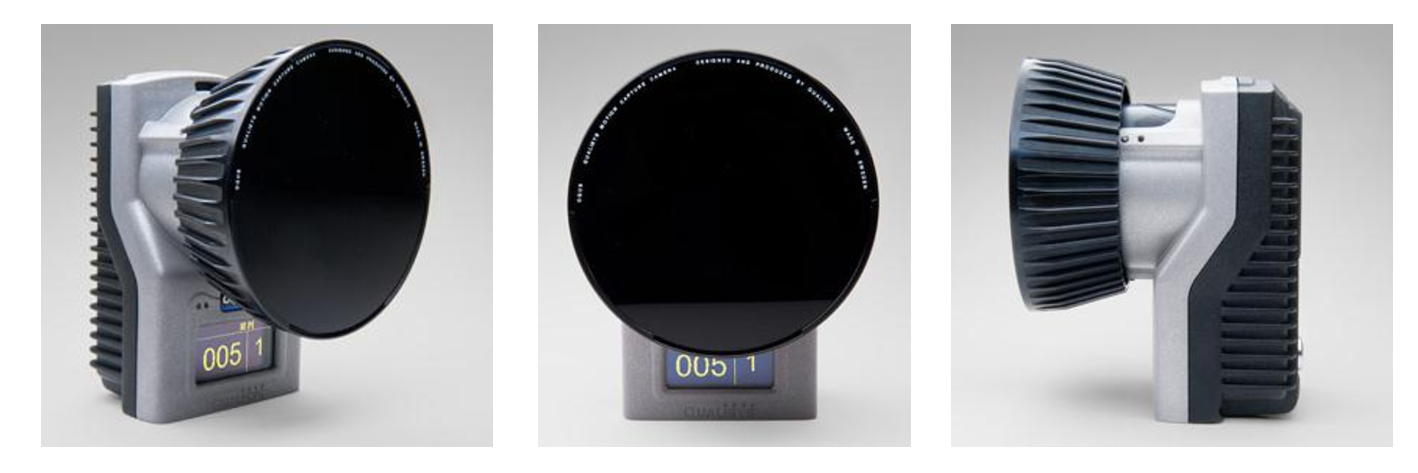
\includegraphics[width=0.7\textwidth]{figures/qs_cameras}
\caption{An Oqus camera part of the Qualisys system.}
\label{fig:qs_cameras}
\end{figure}

\subsection{Computing Euler angles using Qualisys data}
\indent \indent If the subject is wearing two markers per segment, then the pitch angle of such segment is computed between the vector defined by the upper and lower markers and the vector normal to the Earth's surface. To be able to compute it we first have to define a third point which has the same X coordinate as the lower marker and the same Z coordinate as the upper marker. This will define a right triangle in which one of the contiguous cathetus is normal to the Earth's surface and the hypotenuse is defined by the line between the upper and the lower point. Therefore, by calculating the arctangent we can easily find the angle of the right triangle, which is, in turn, the pitch angle. Figure \ref{fig:pitch_triangle} shows this process.

\begin{figure}[H]
\centering
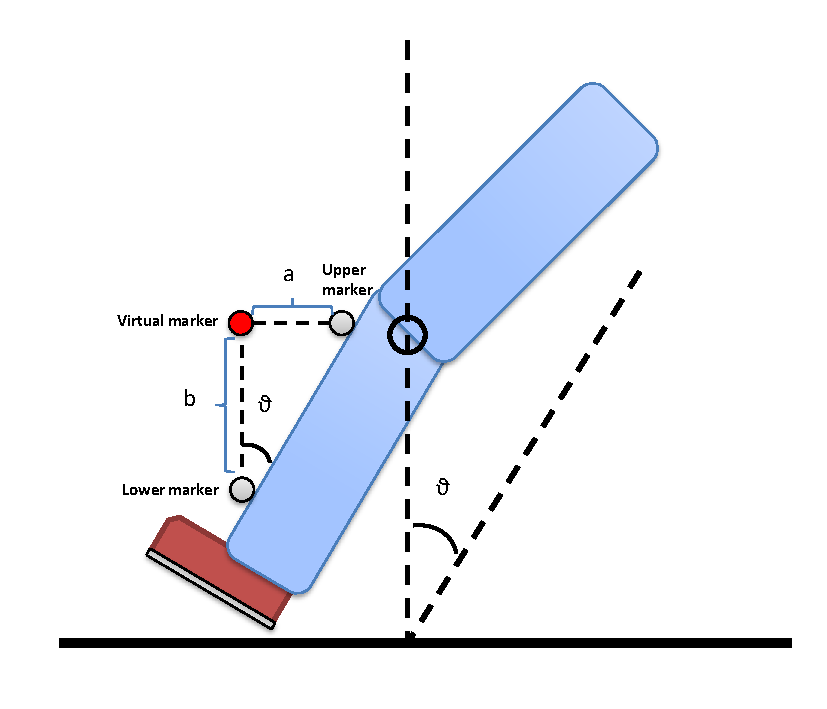
\includegraphics[width=0.7\textwidth]{figures/qualisys_pitch}
\caption{Diagram of the pitch computation using the Qualisys system.}
\label{fig:pitch_triangle}
\end{figure}

\indent Therefore, the pitch angle is computed applying,

\begin{gather}
\theta = \arctan\left(\frac{a}{b}\right)\\
a=\sqrt{\left(x_{upper}-x_{lower}\right)^2+\left(z_{upper}-z_{upper}\right)^2}\\
b=\sqrt{\left(x_{lower}-x_{lower}\right)^2+\left(z_{lower}-z_{upper}\right)^2}
\label{eq:qs_pitch}
\end{gather}

where $[x_{lower},z_{lower}]$ and $[x_{upper},z_{upper}]$ are the coordinates of the projections of the lower and upper markers in the XZ plane, respectively.

\section{Qualisys validation experiments}
\subsection{Data gathering protocol}
\begin{itemize}
\item Switch on the computer.
\item Switch on the Qualisys system.
\item Start the computer and select the "Tracking" account.
\item Write any password, the system will say that the password is wrong and it will show the secret question. The answer to the secret question is "tracking".
\item Once the session has started, open the "Qualisys Track Manager". 
\item Place the calibration frame (which is in the big metallic box and has an L shape) on the floor. 
\item Press the red button and check that the maximum number of cameras see the four markers which are attached to the calibration frame. You may need to adjust the position of the cameras. The cameras also have a small display which show the ID of the camera and the number of markers which are seen in each instant.
\item When all the cameras are ready, go to "capture$\rightarrow$calibrate". Select the desired delay and the desired calibration time (30 seconds should be fine). 
\item Grab the calibration wand (the device which is shaped as a T), click the button to start the calibration and move around the room moving the wand trying to cover all the space.
\item When the calibration is done, hide both the calibration frame and the calibration wand somewhere where the markers are not seen by the cameras (you may need to put them back into the big metallic box or just put them out of the room).
\item The system is now ready to start the measurements.
\item Place the GaitWatch system on the subject and place the markers on the desired segments of the subject. 
\item Press the red button (new capture) and complete the required fields: initial delay, number of samples (200 by default), duration and name of the file. 
\item Before starting the capture, switch on the GaitWatch system and press the button to start the measurement. Tell the subject to stay static.
\item Go back to the computer, start the capture and write down the current time together with the name you have given to the file. 
\item The subject may now move around the room and carry out the movements he is instructed to. 
\item When the capture is done, press the GaitWatch button again to stop the measurement. 
\item Go back to the computer and label one by one all the markers that were identified by the program. This is done by clicking on the markers, going to "identify$\rightarrow$label. 
\item Once all the markers are identified, save the file and go to "file$\rightarrow$export$\rightarrow$MAT", then click OK. This will export all the data to a .mat file. Be careful because the .mat file is created when we start a new capture but it will remain empty until the exportation. 
\end{itemize}

The next step would be to download the GaitWatch data to the computer. To do so we use the \textit{GW\_comm.m} routine. This routine will also ask the user to give each one of the files a number. Be sure to give the file the same number which was given to the Qualisys file. Once all the data are identified, we can run the \textit{param\_optimization.m} routine which loads both the GaitWatch and Qualisys data, synchronizes them and computes the optimal parameters of the algorithm used to compute the orientation using the GaitWatch data. \\

\indent The following sections contain a set of figures depicting the pitch angle of different segments computed using both the Qualisys and the GaitWatch systems. 

\section{Fast Walking}

\begin{figure}[H]
\centering
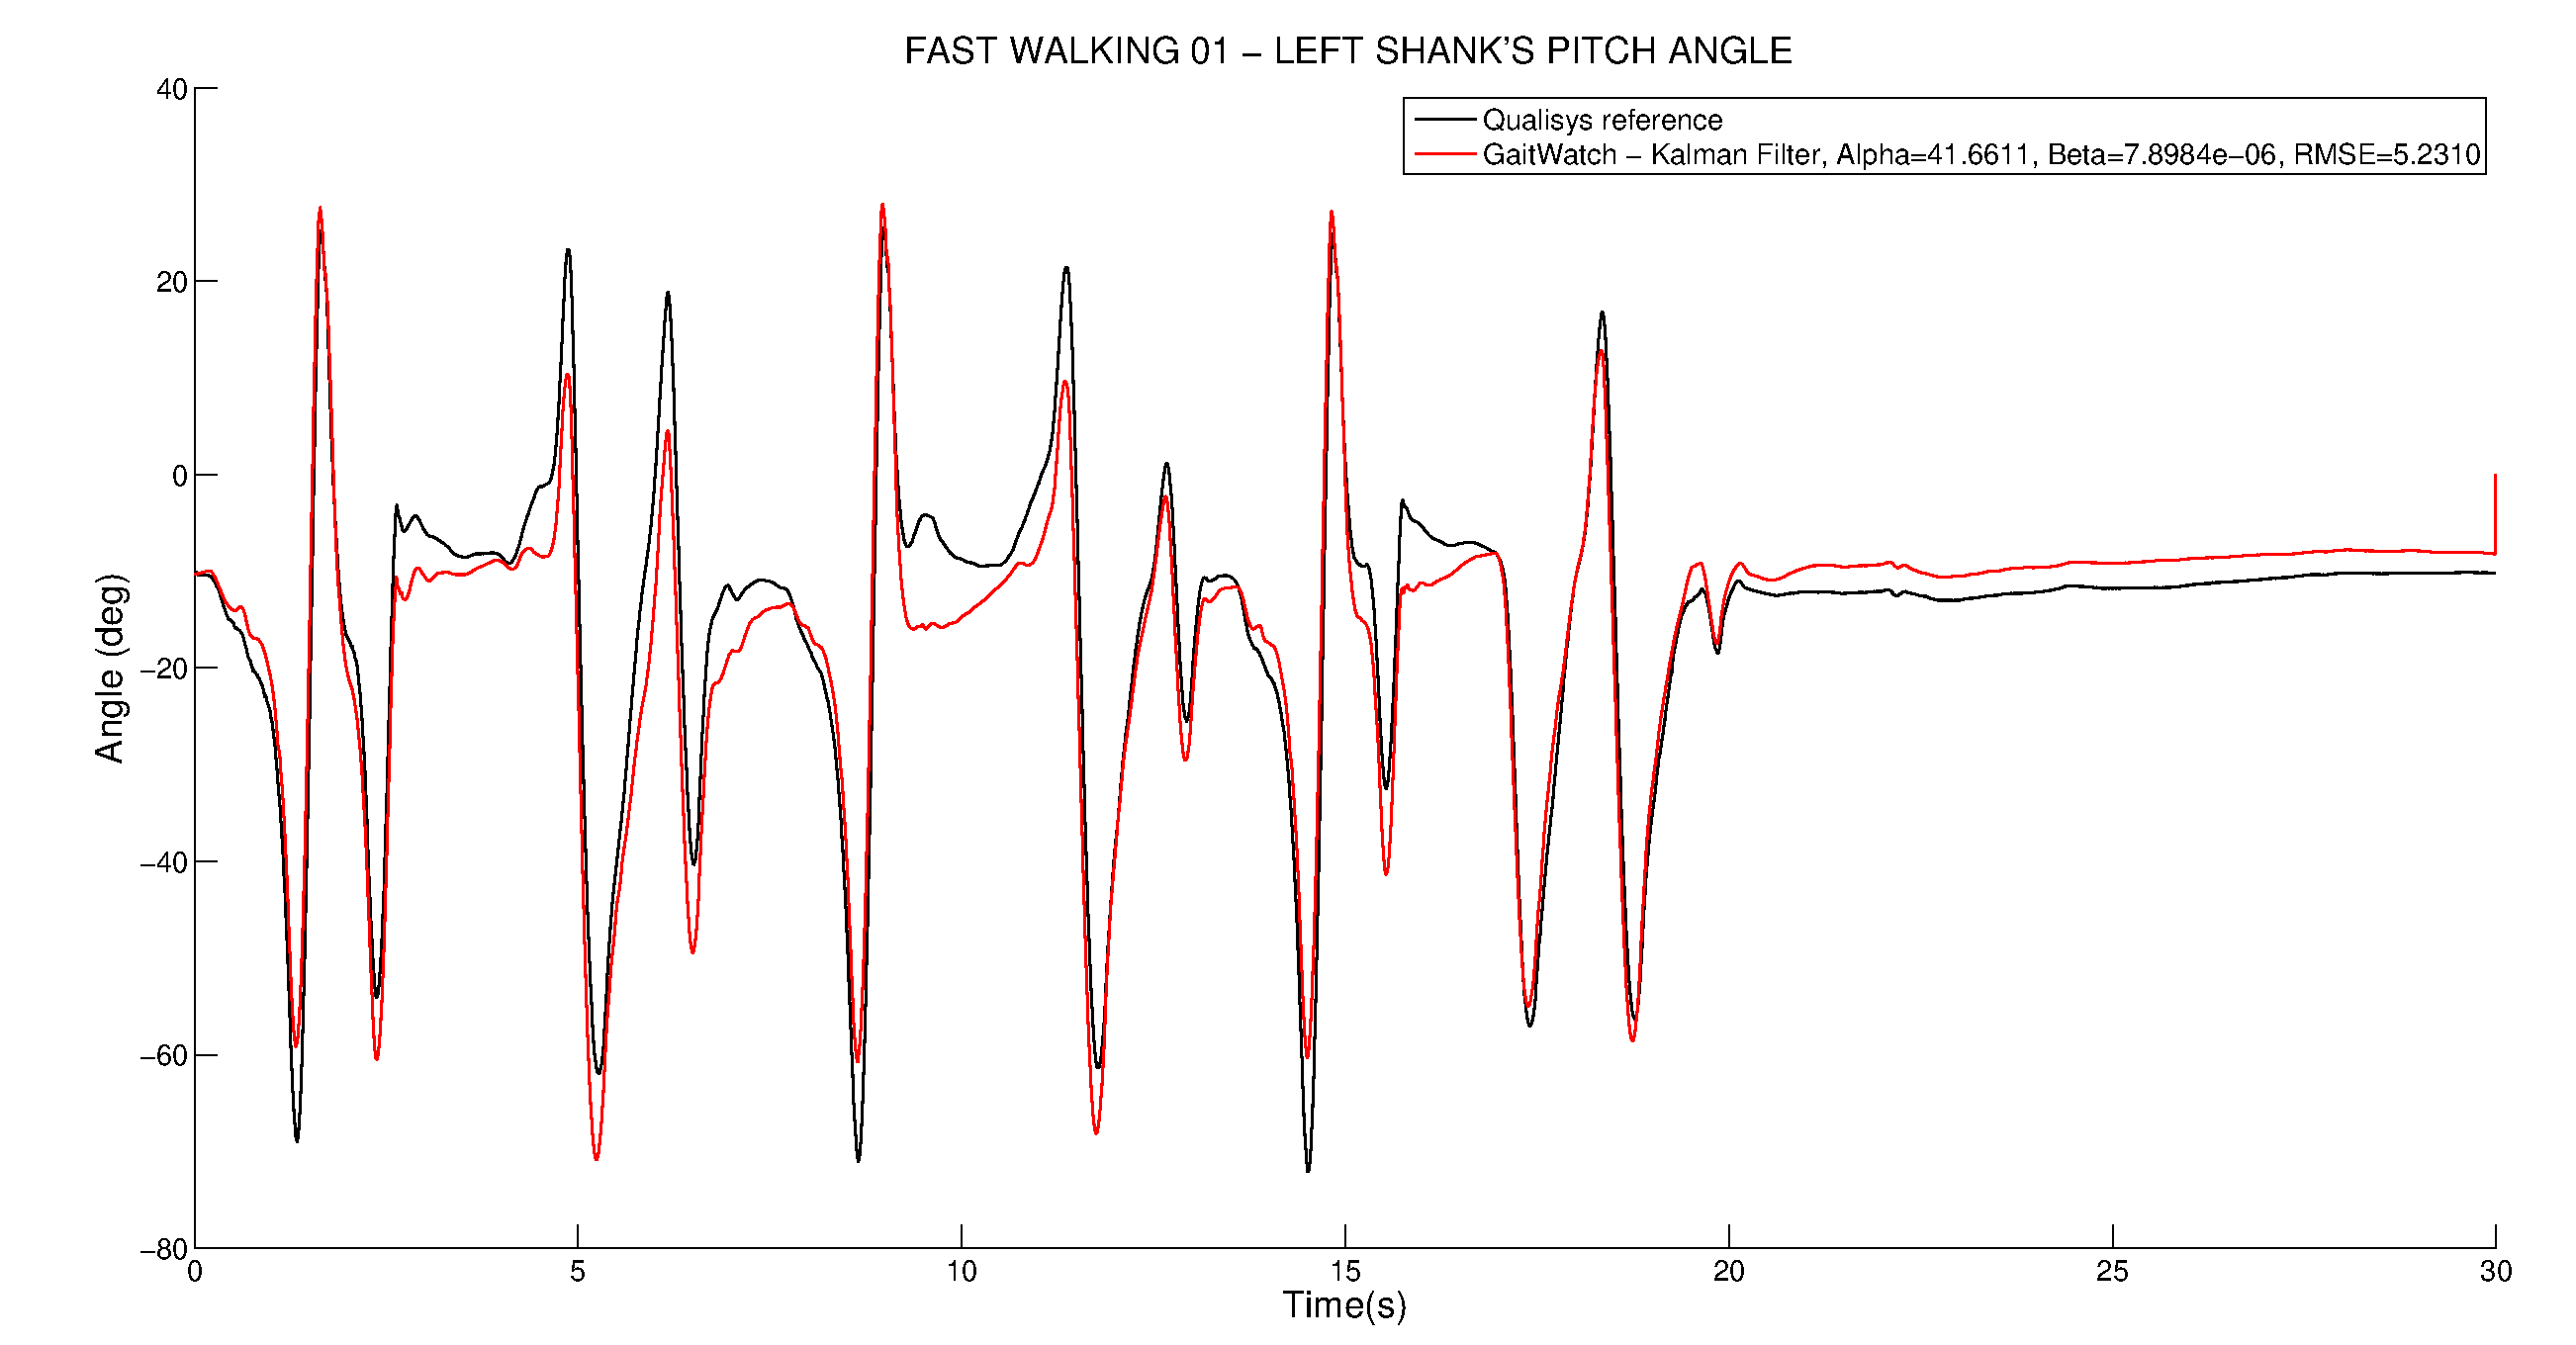
\includegraphics[width=1\textwidth]{figures/fast_walking_01_left_shank.eps}
\caption{Pitch angle of left shank measured while walking fast (GaitWatch vs. Qualisys).}
\label{fig:fast_walking_left_shank01}
\end{figure}

\begin{figure}[H]
\centering
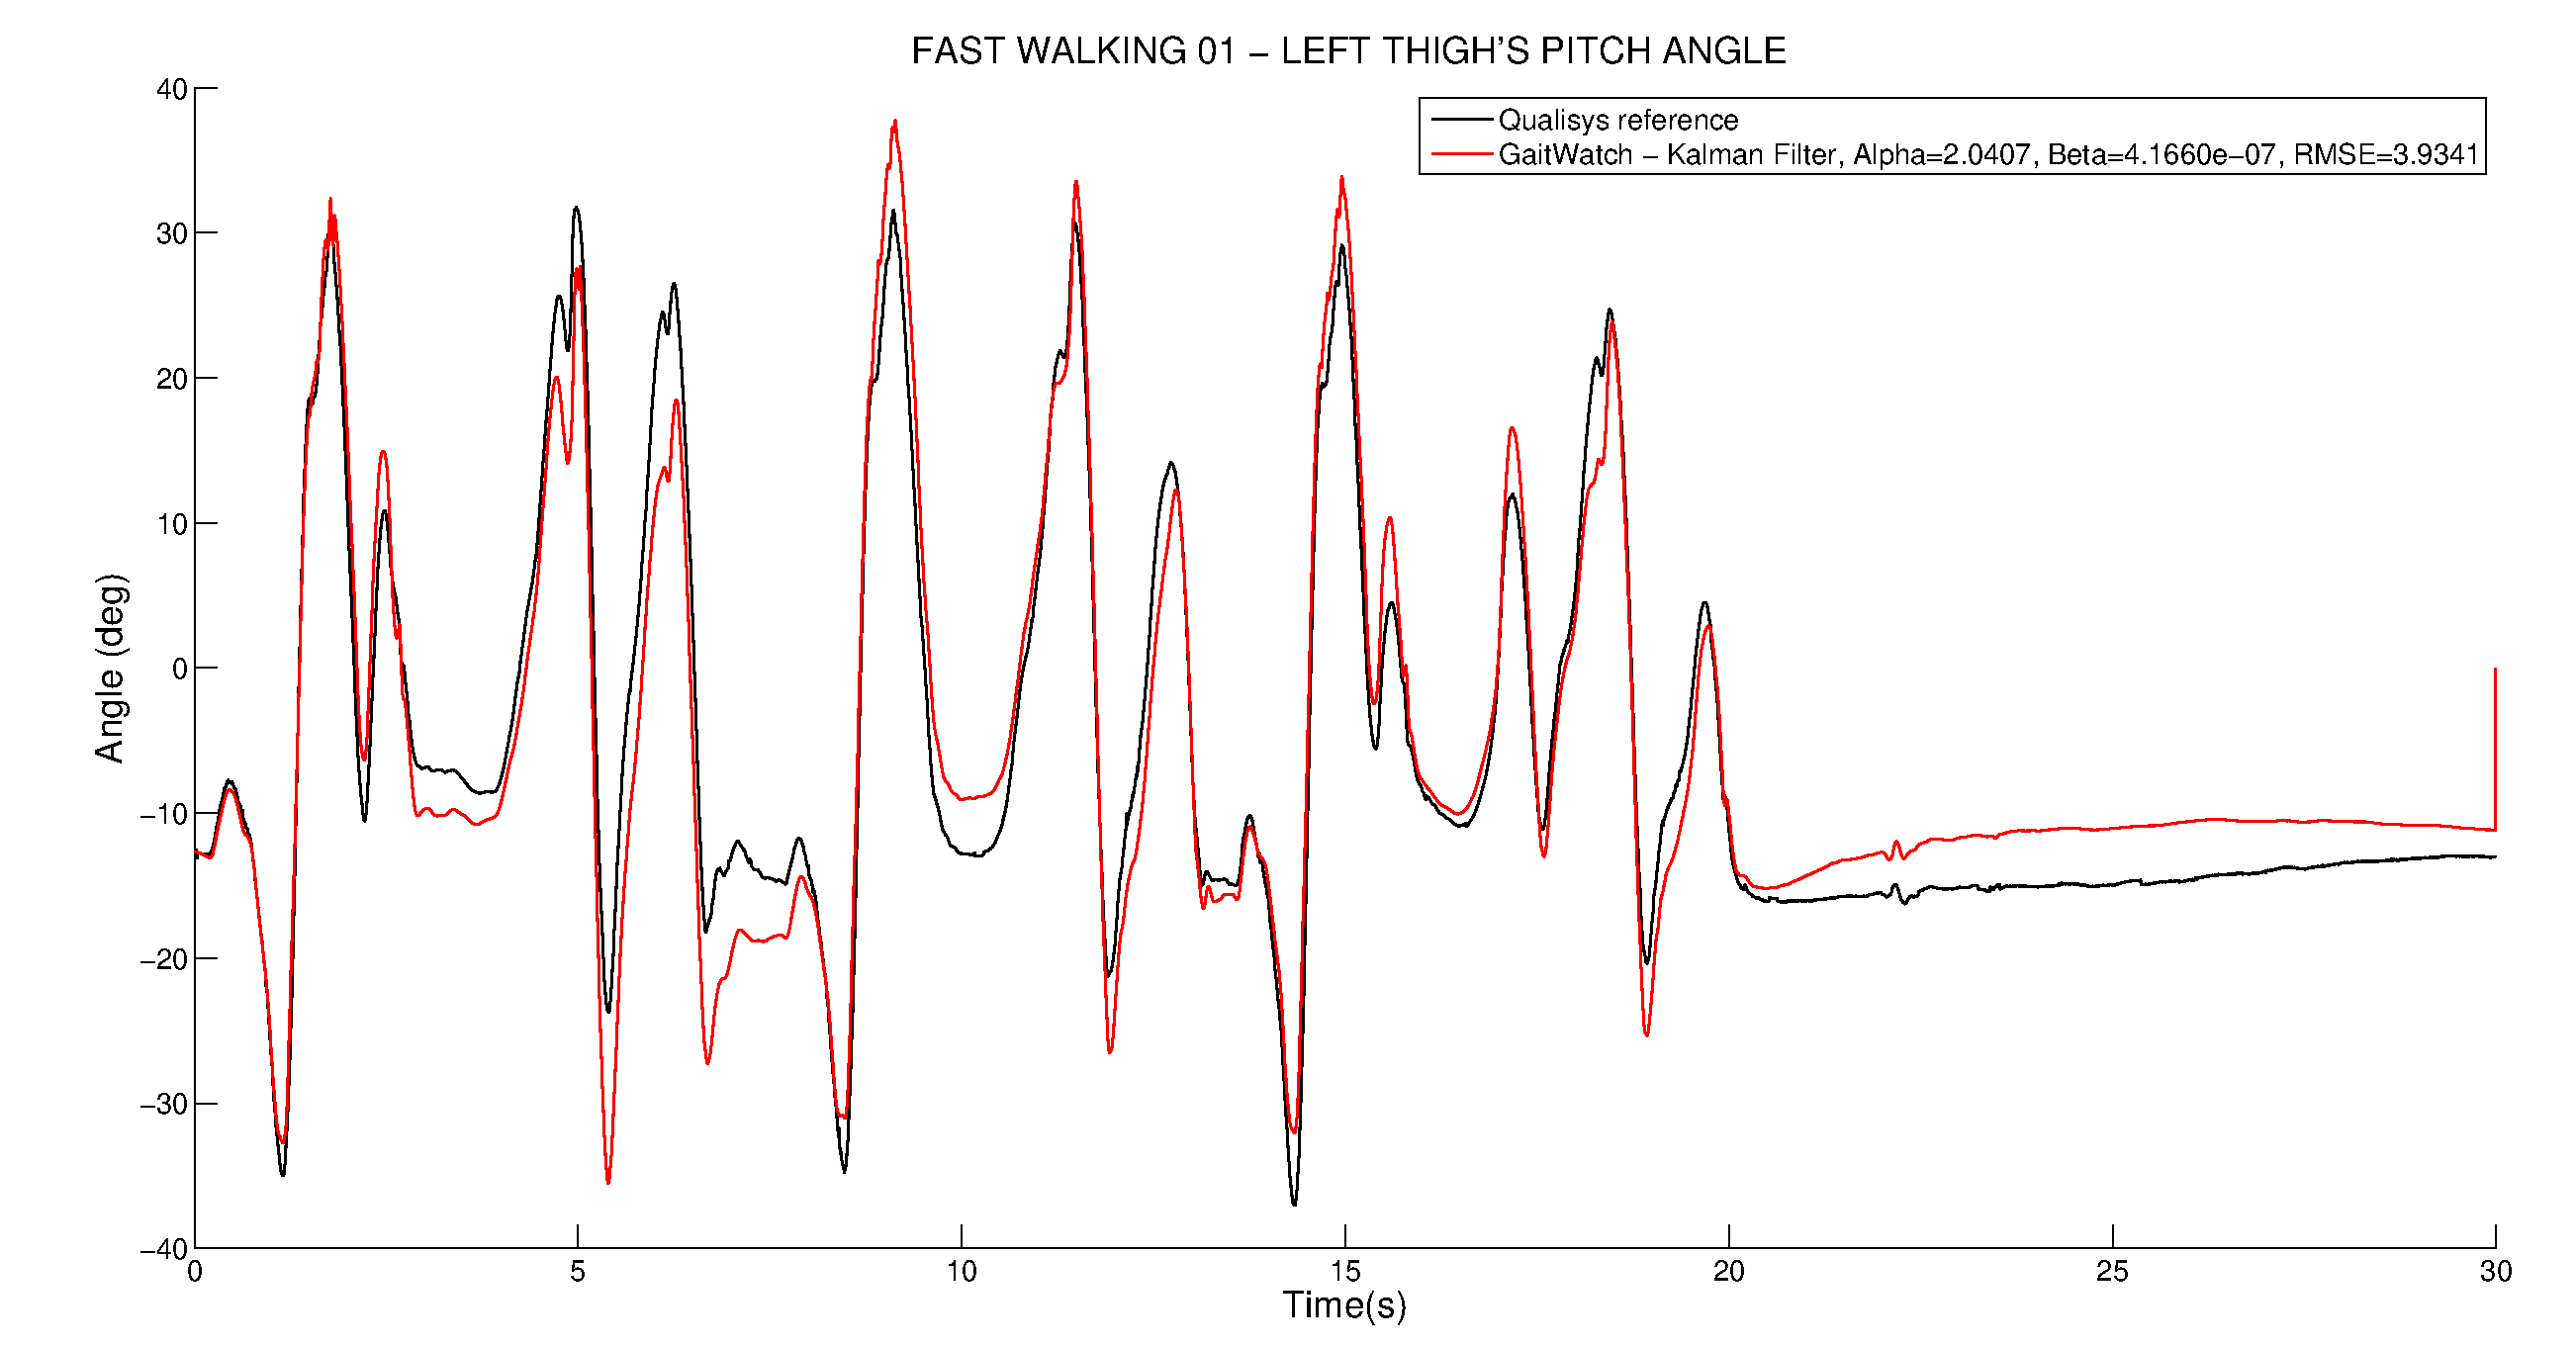
\includegraphics[width=1\textwidth]{figures/fast_walking_01_left_thigh.eps}
\caption{Pitch angle of left thigh measured while walking fast (GaitWatch vs. Qualisys).}
\label{fig:fast_walking_left_thigh01}
\end{figure}

\begin{figure}[H]
\centering
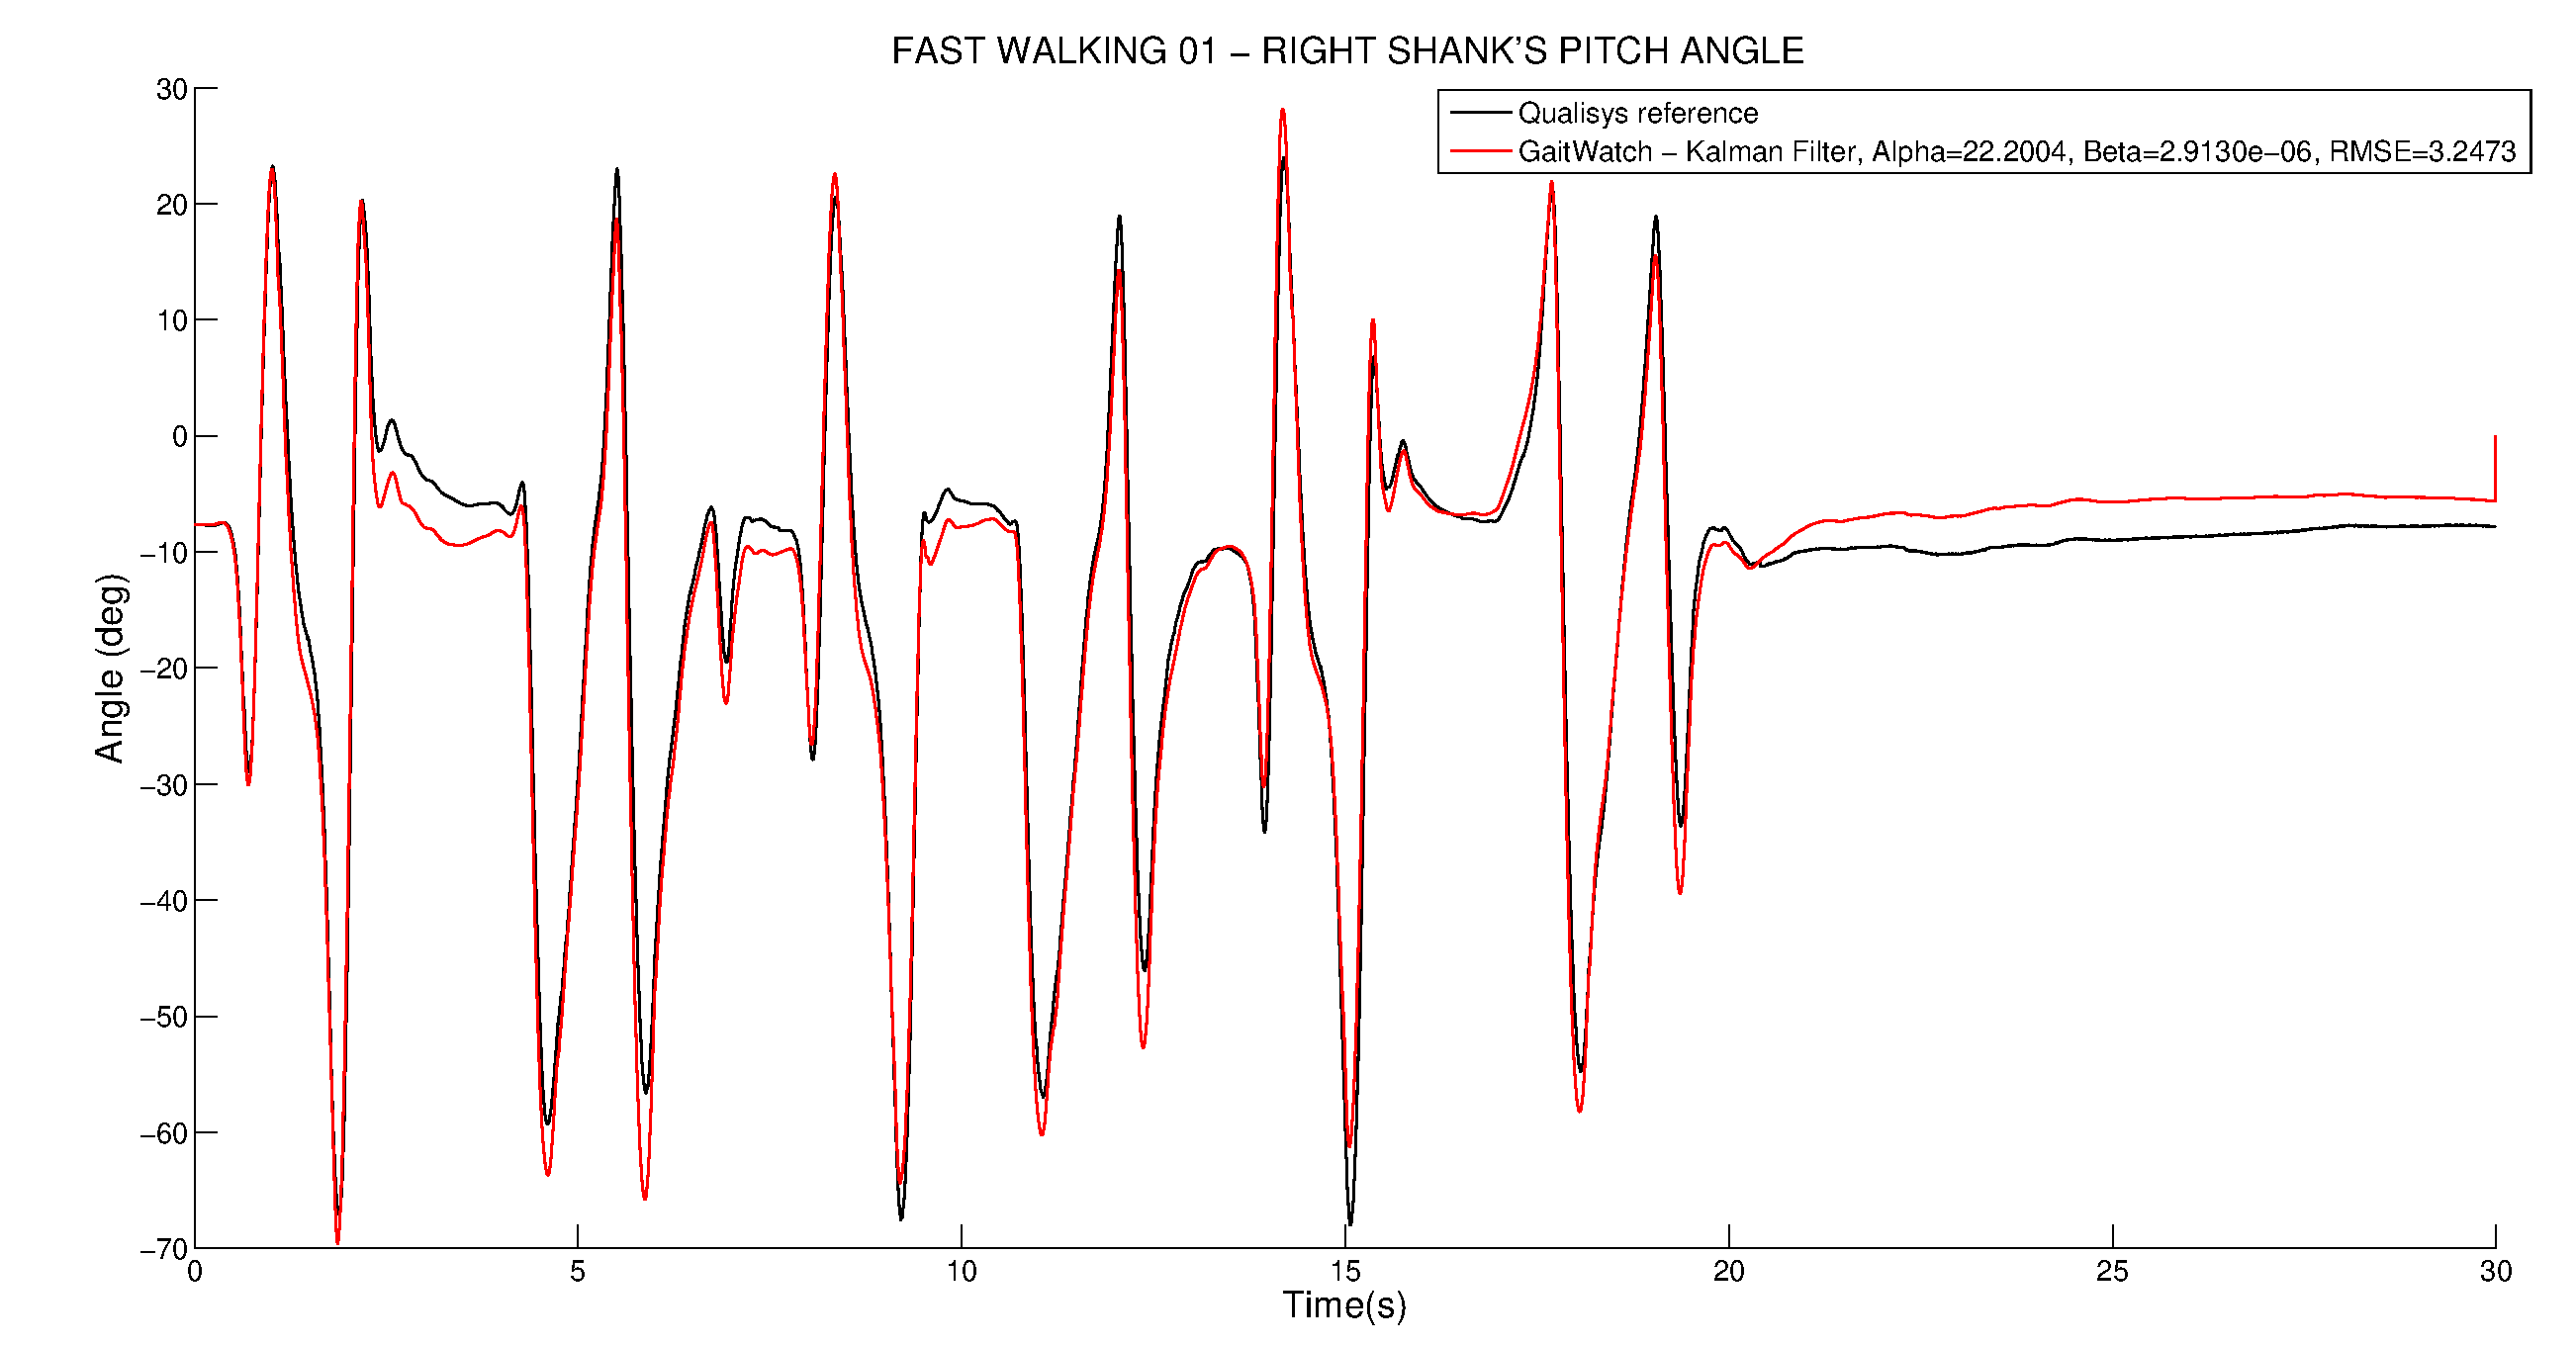
\includegraphics[width=1\textwidth]{figures/fast_walking_01_right_shank.eps}
\caption{Pitch angle of right shank measured while walking fast (GaitWatch vs. Qualisys).}
\label{fig:fast_walking_right_shank01}
\end{figure}

\begin{figure}[H]
\centering
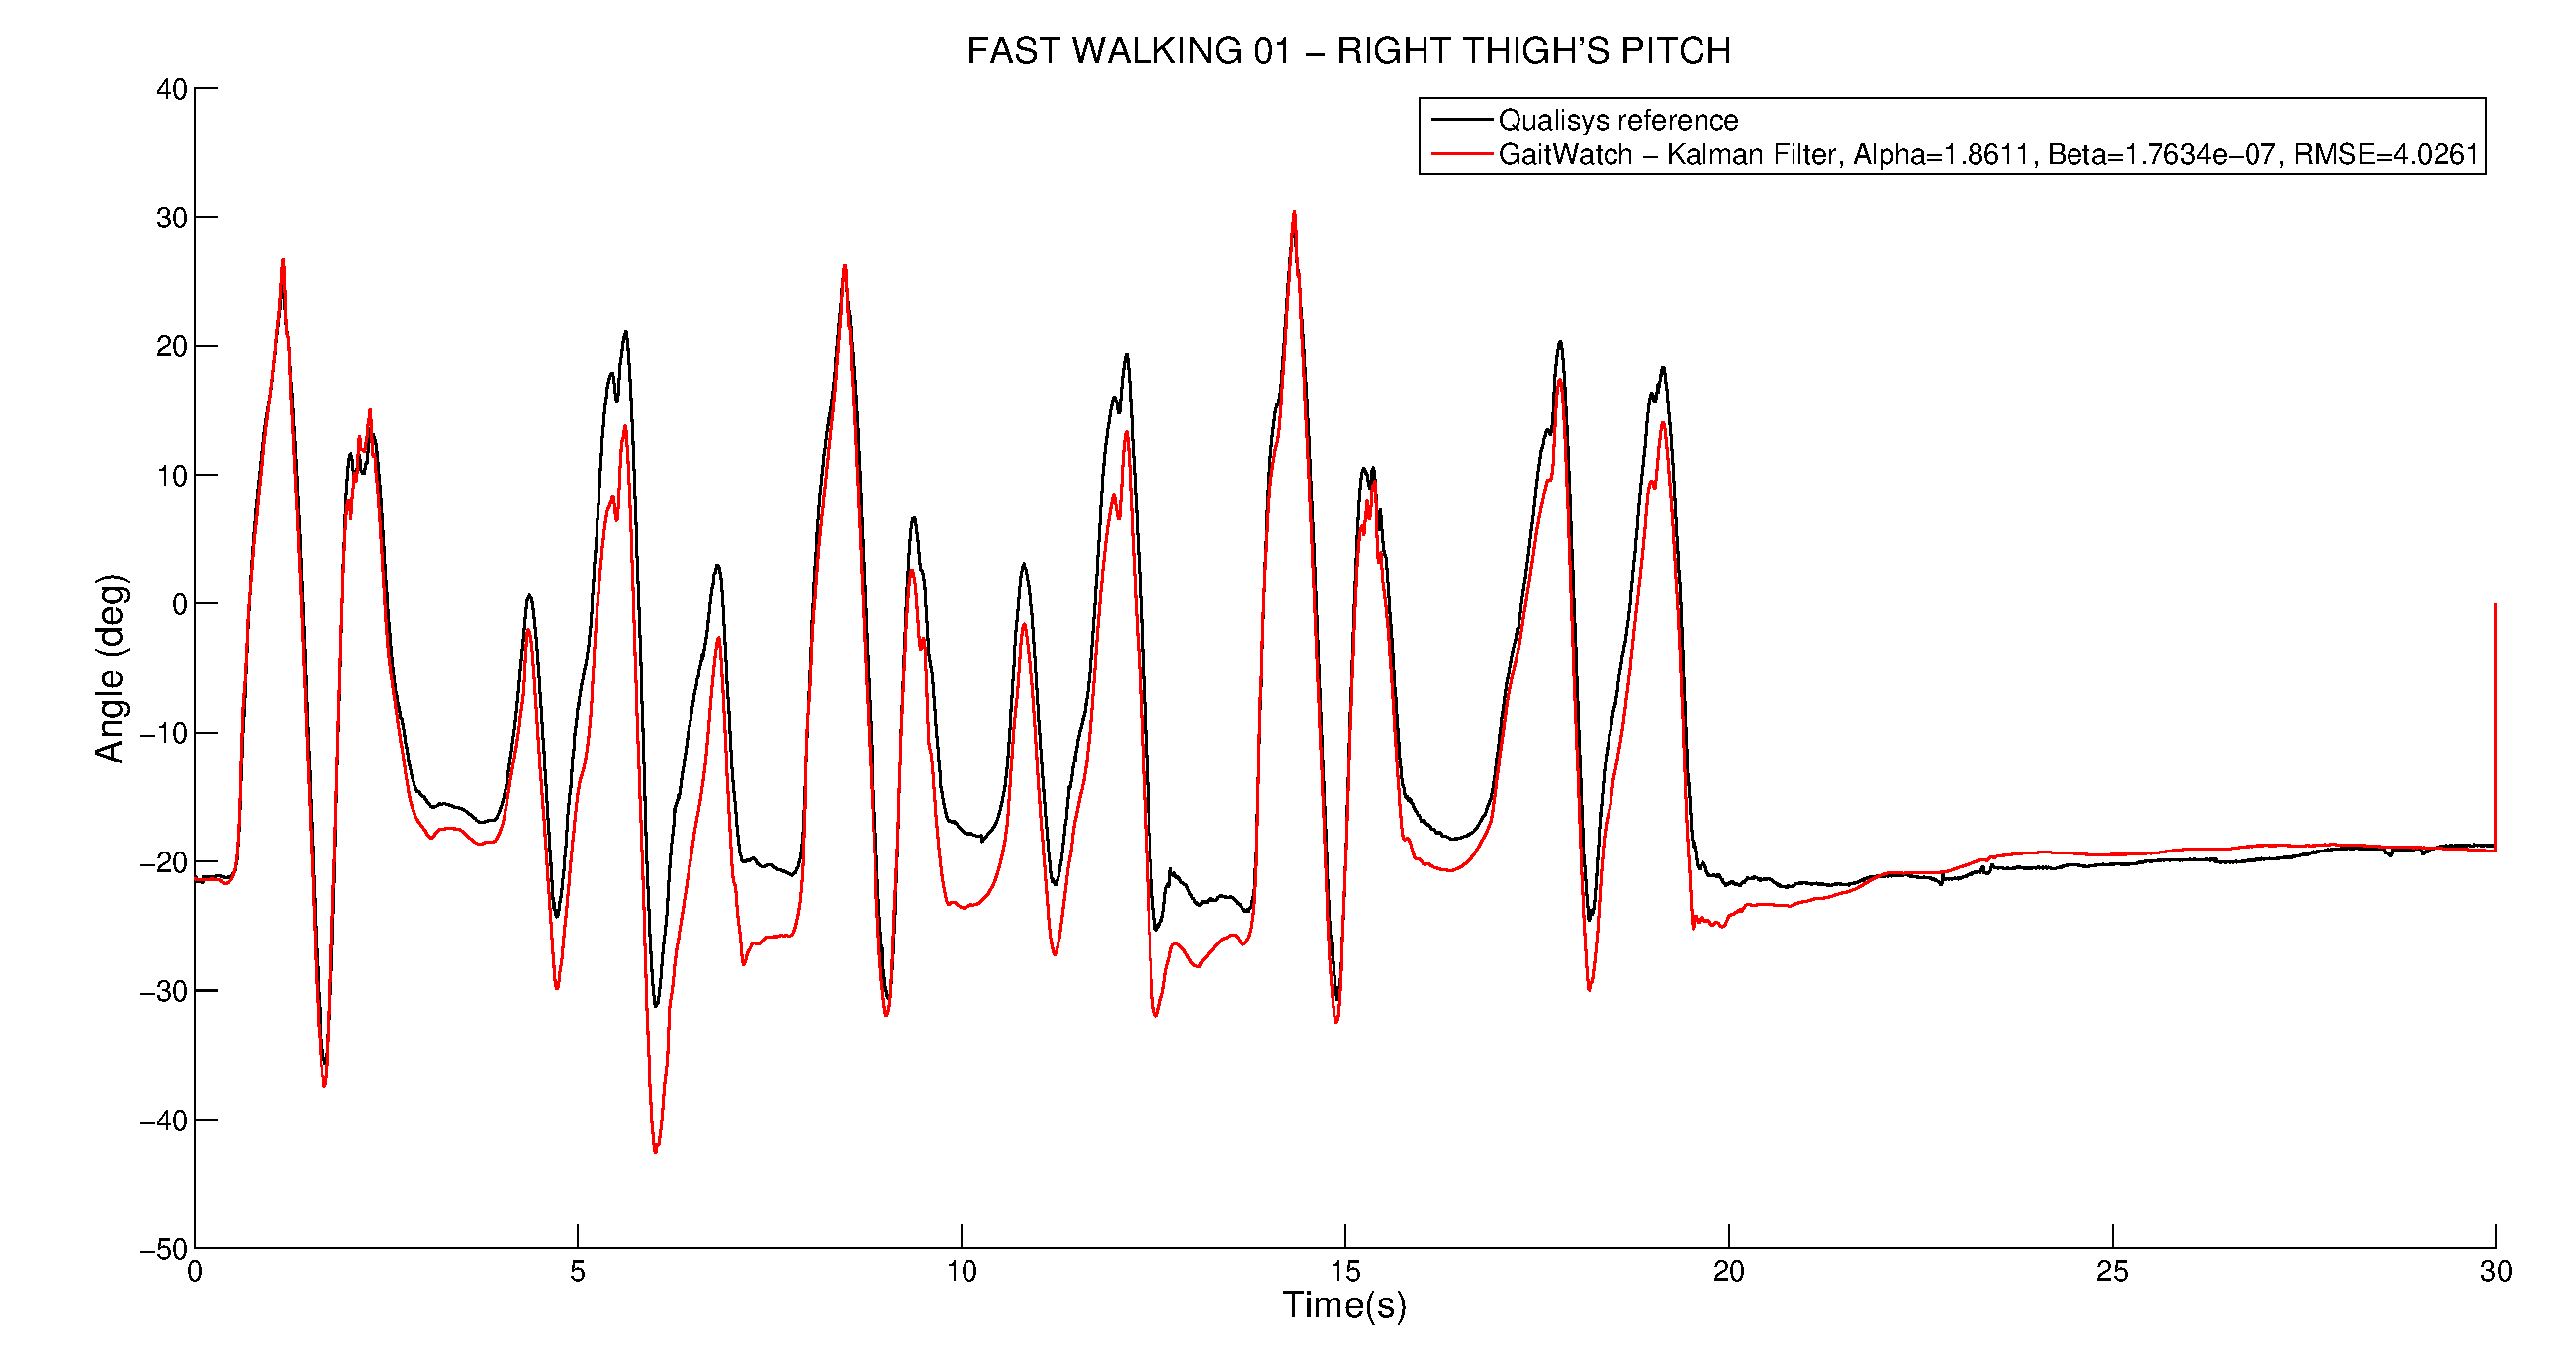
\includegraphics[width=1\textwidth]{figures/fast_walking_01_right_thigh.eps}
\caption{Pitch angle of right thigh measured while walking fast (GaitWatch vs. Qualisys).}
\label{fig:fast_walking_right_thigh01}
\end{figure}

\section{Jumping}

\begin{figure}[H]
\centering
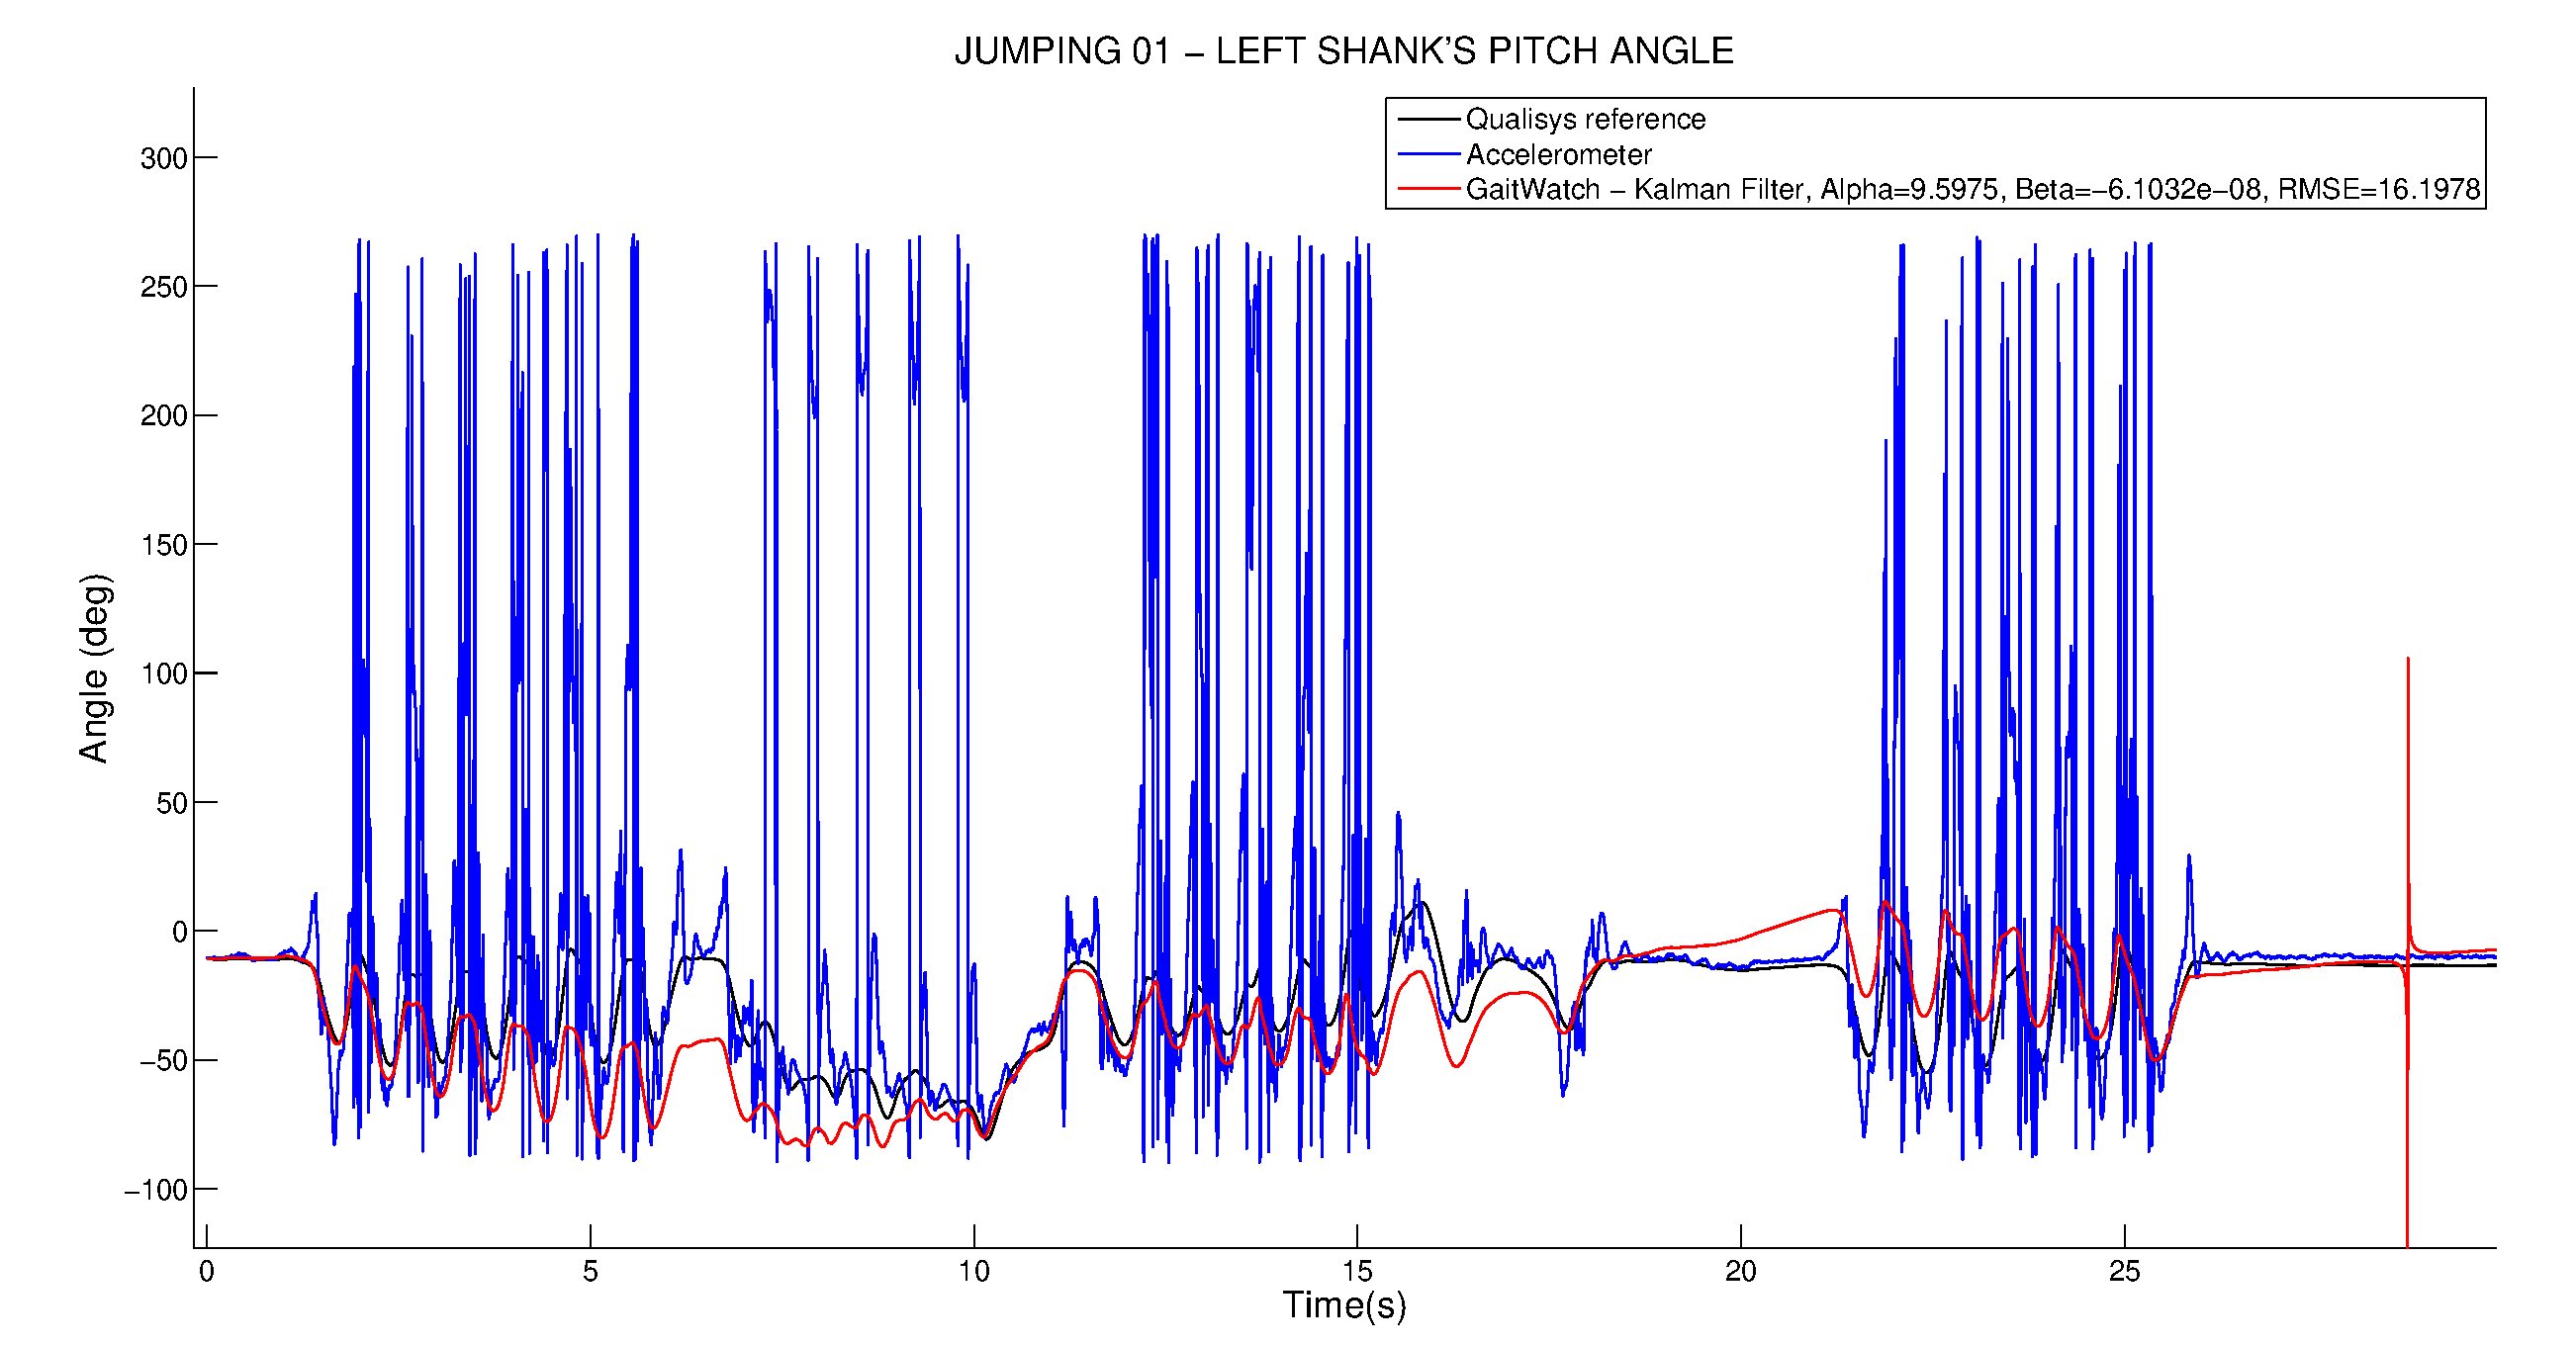
\includegraphics[width=1\textwidth]{figures/jumping_01_left_shank_with_acc.eps}
\caption{Pitch angle of left shank measured while jumping (GaitWatch vs. Qualisys).}
\label{fig:jumping_left_shank01}
\end{figure}

\begin{figure}[H]
\centering
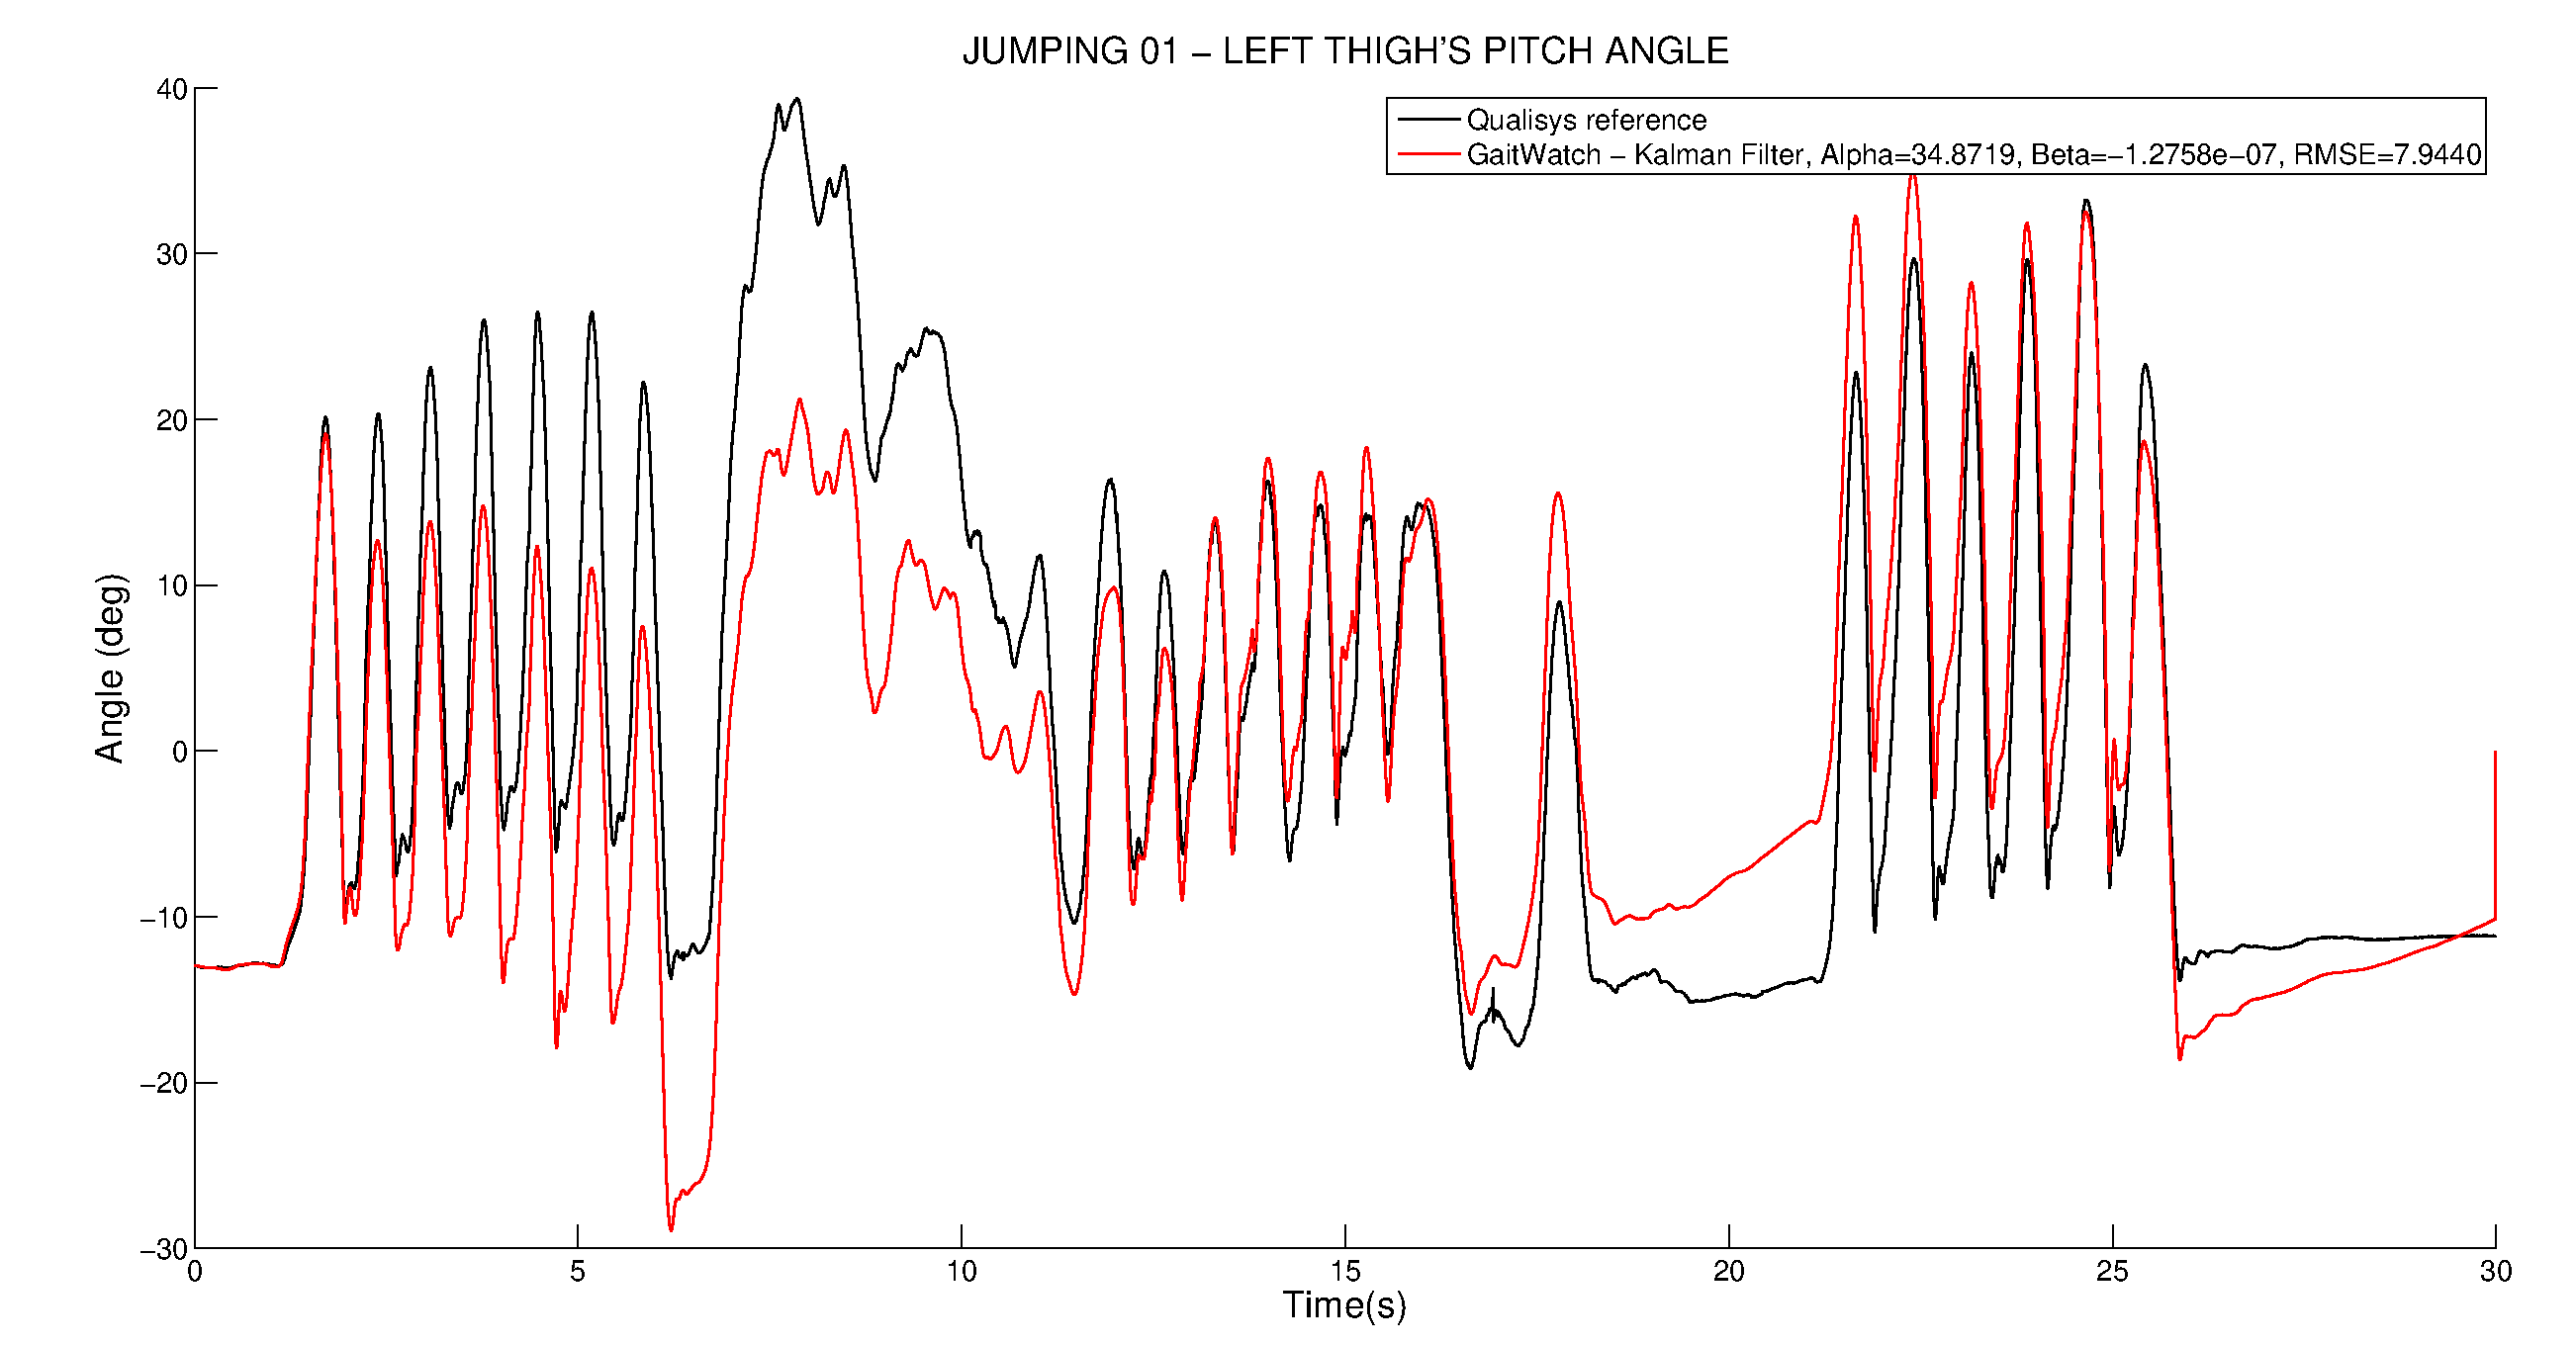
\includegraphics[width=1\textwidth]{figures/jumping_01_left_thigh.eps}
\caption{Pitch angle of left thigh measured while jumping (GaitWatch vs. Qualisys).}
\label{fig:jumping_left_thigh01}
\end{figure}

\begin{figure}[H]
\centering
\includegraphics[width=1\textwidth]{figures/jumping_01_right_shank.eps}
\caption{Pitch angle of right shank measured while jumping (GaitWatch vs. Qualisys).}
\label{fig:jumping_right_shank01}
\end{figure}

\begin{figure}[H]
\centering
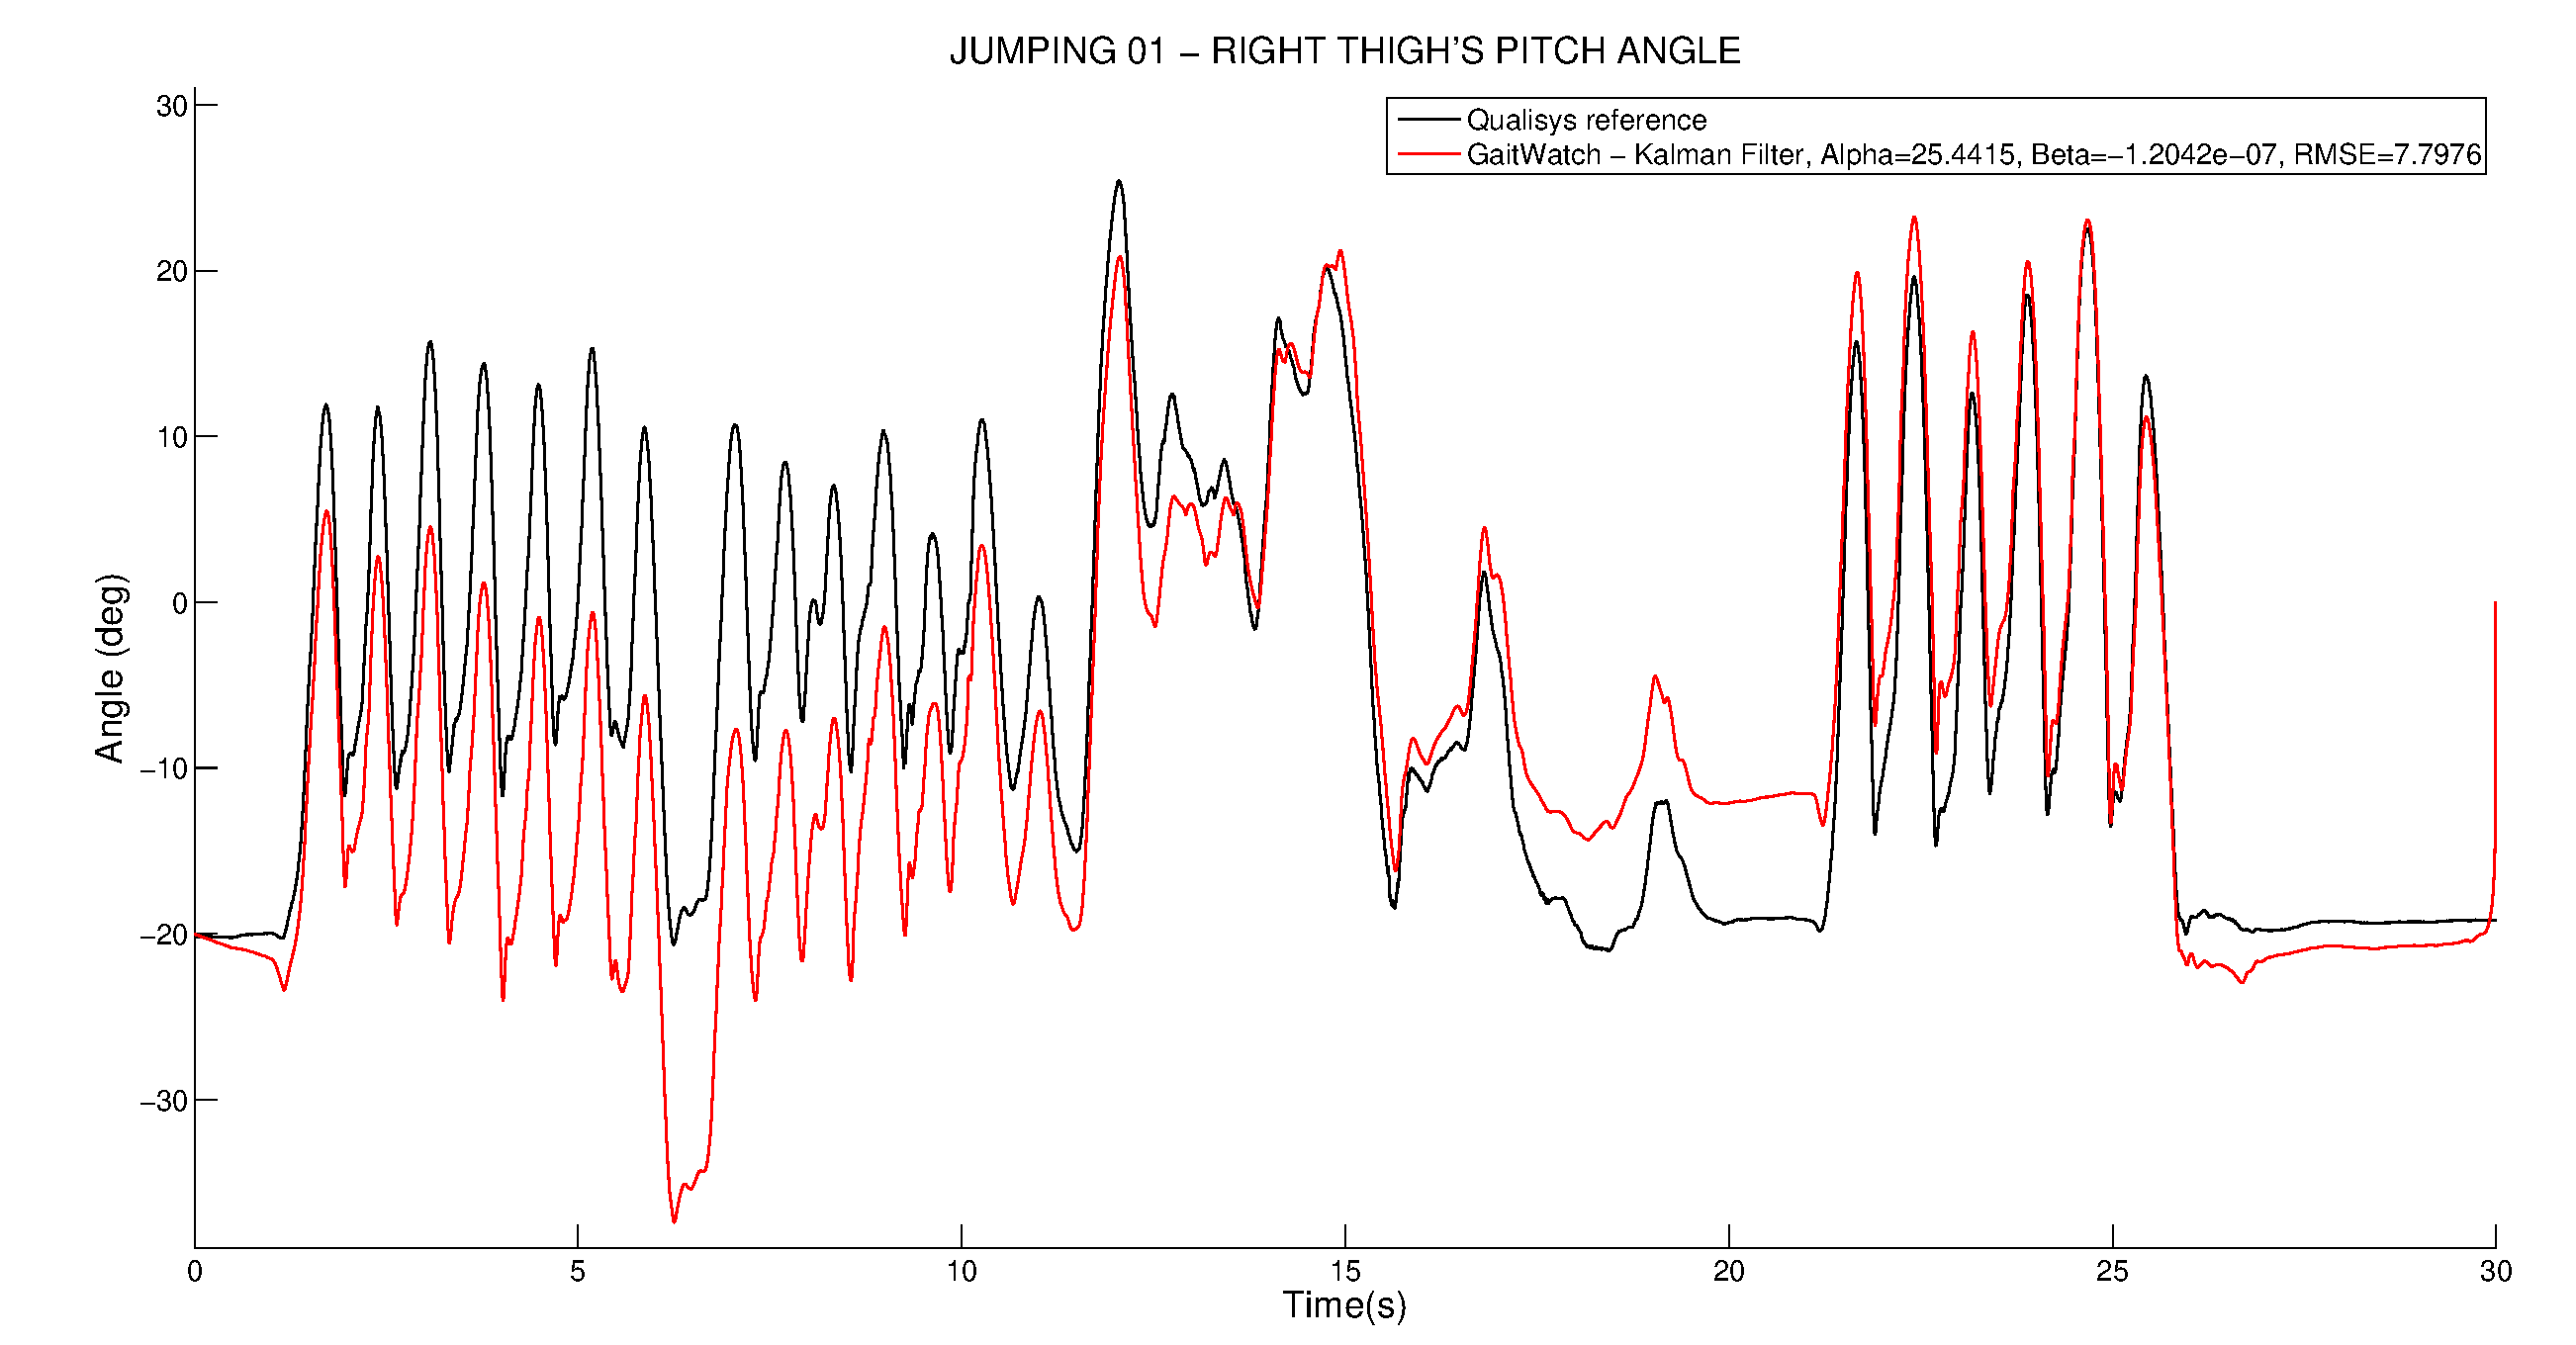
\includegraphics[width=1\textwidth]{figures/jumping_01_right_thigh.eps}
\caption{Pitch angle of right thigh measured while jumping (GaitWatch vs. Qualisys).}
\label{fig:jumping_right_thigh01}
\end{figure}

\section{Leg motion}

\begin{figure}[H]
\centering
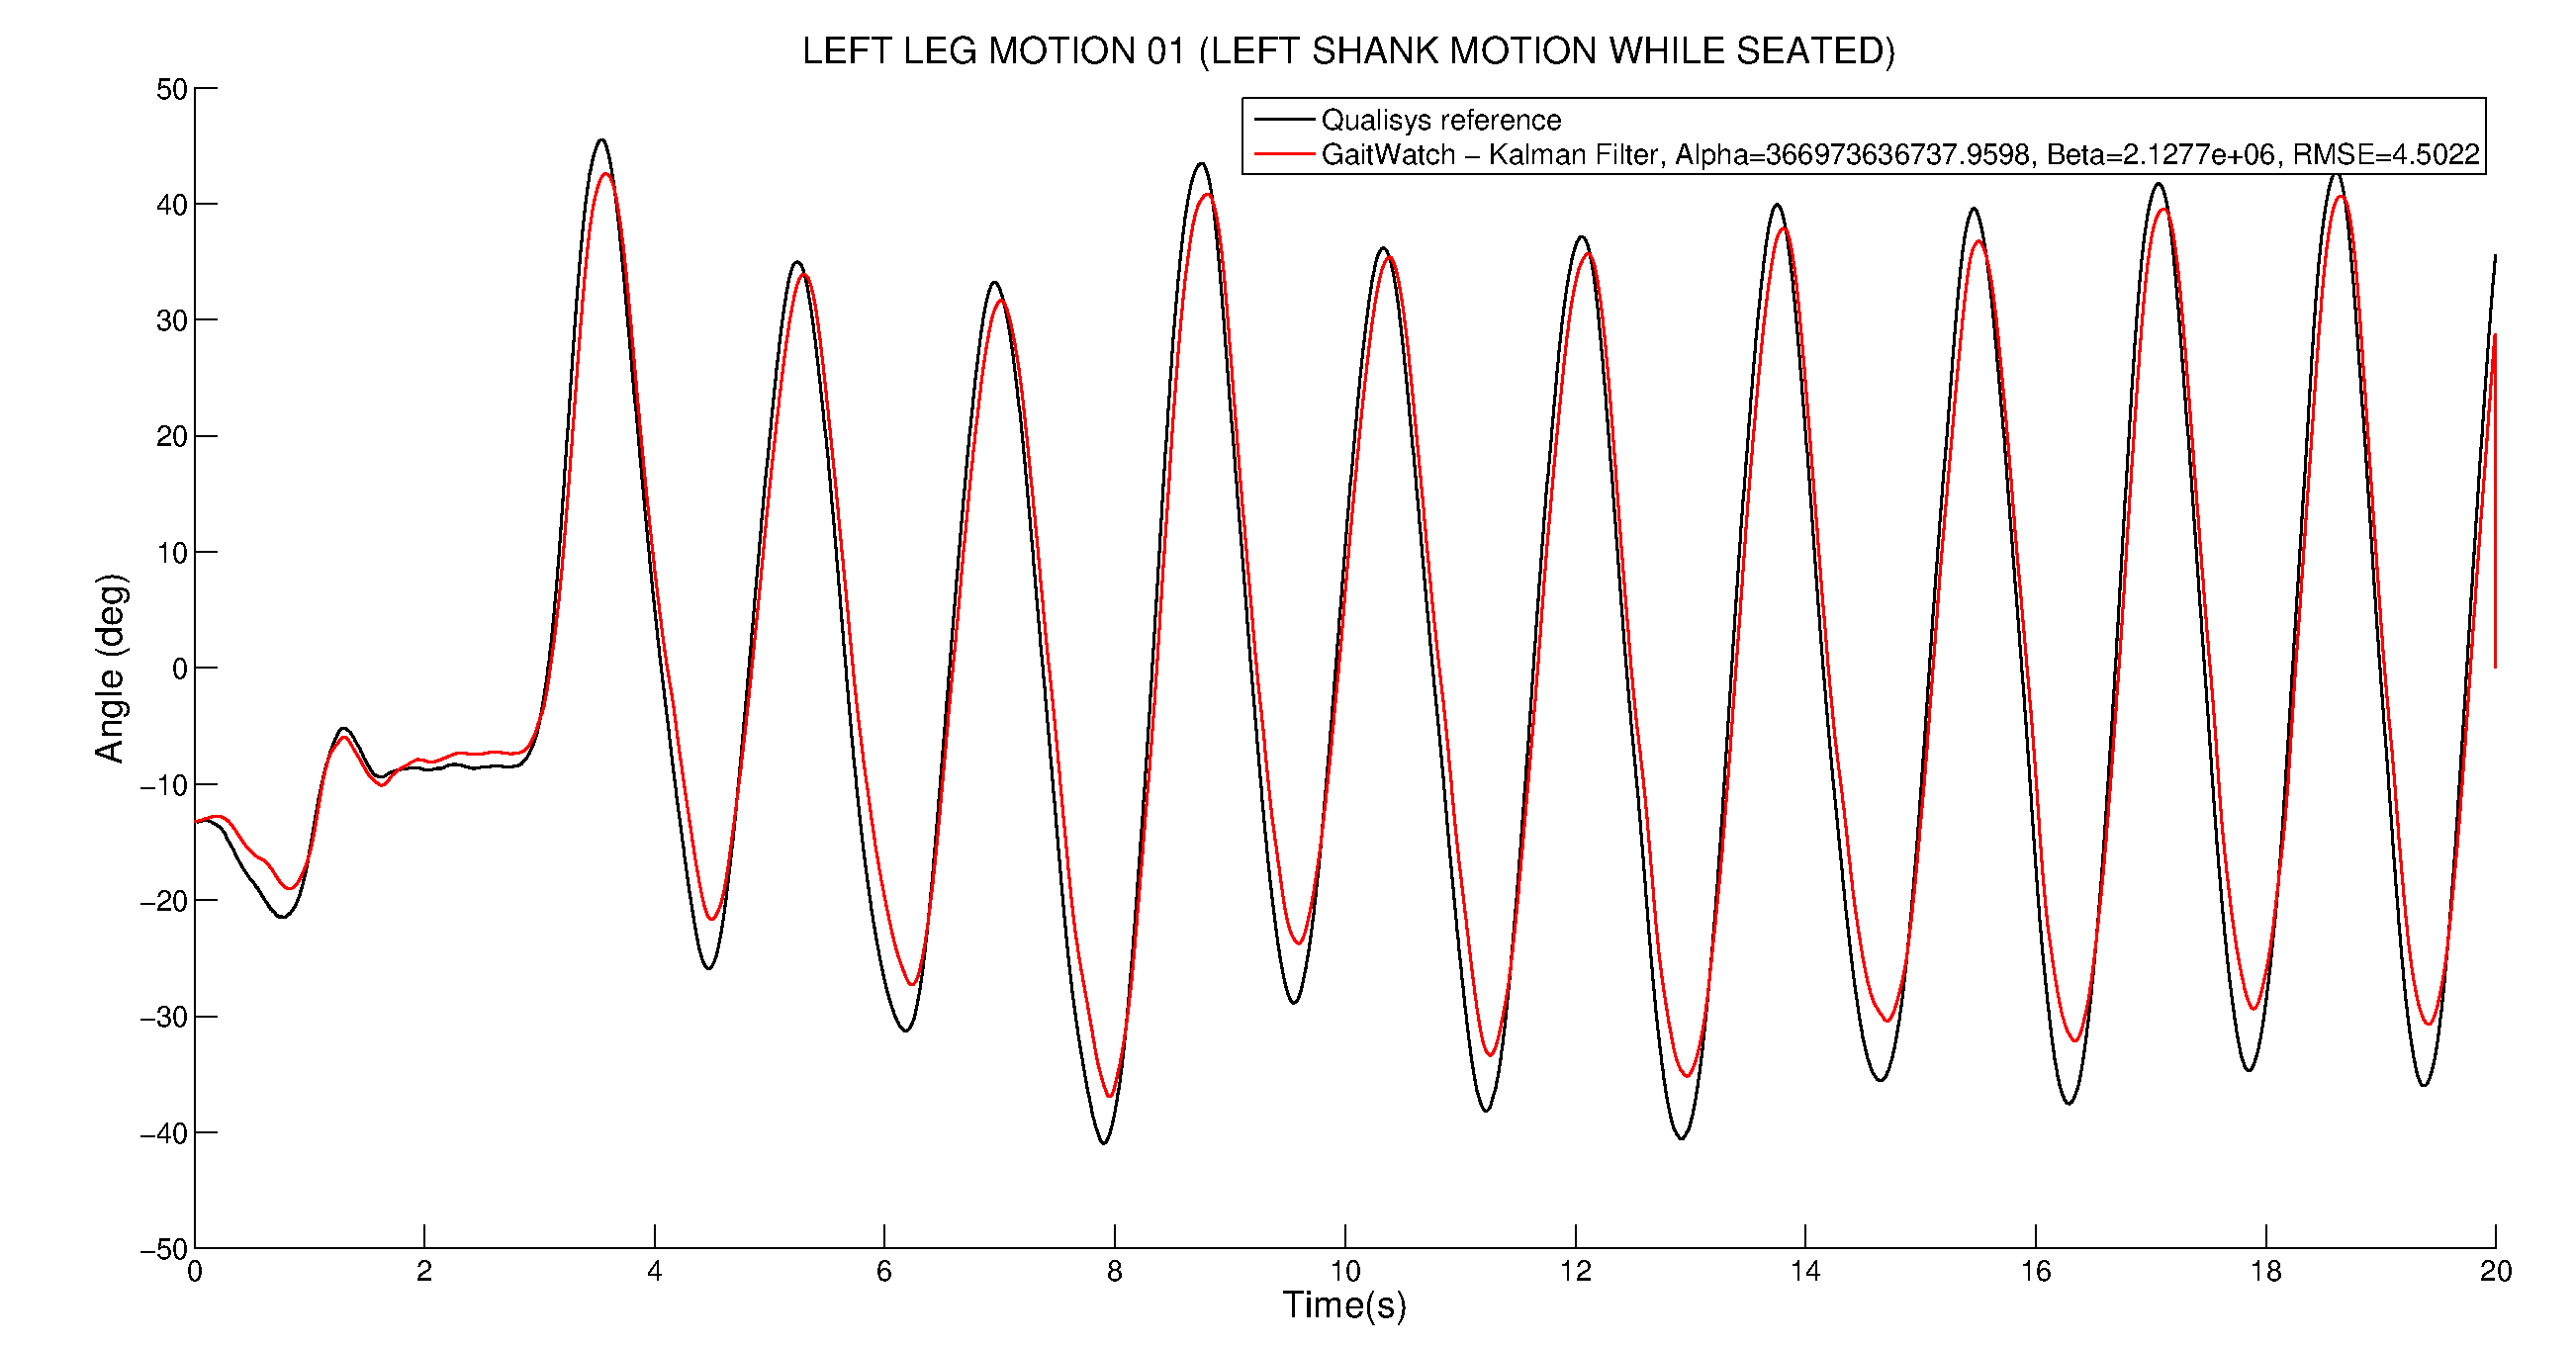
\includegraphics[width=1\textwidth]{figures/Left_leg_motion_01_shank.eps}
\caption{Pitch angle while swinging left shank. (GaitWatch vs. Qualisys).}
\label{fig:Left_leg_motion_01_shank}
\end{figure}

\begin{figure}[H]
\centering
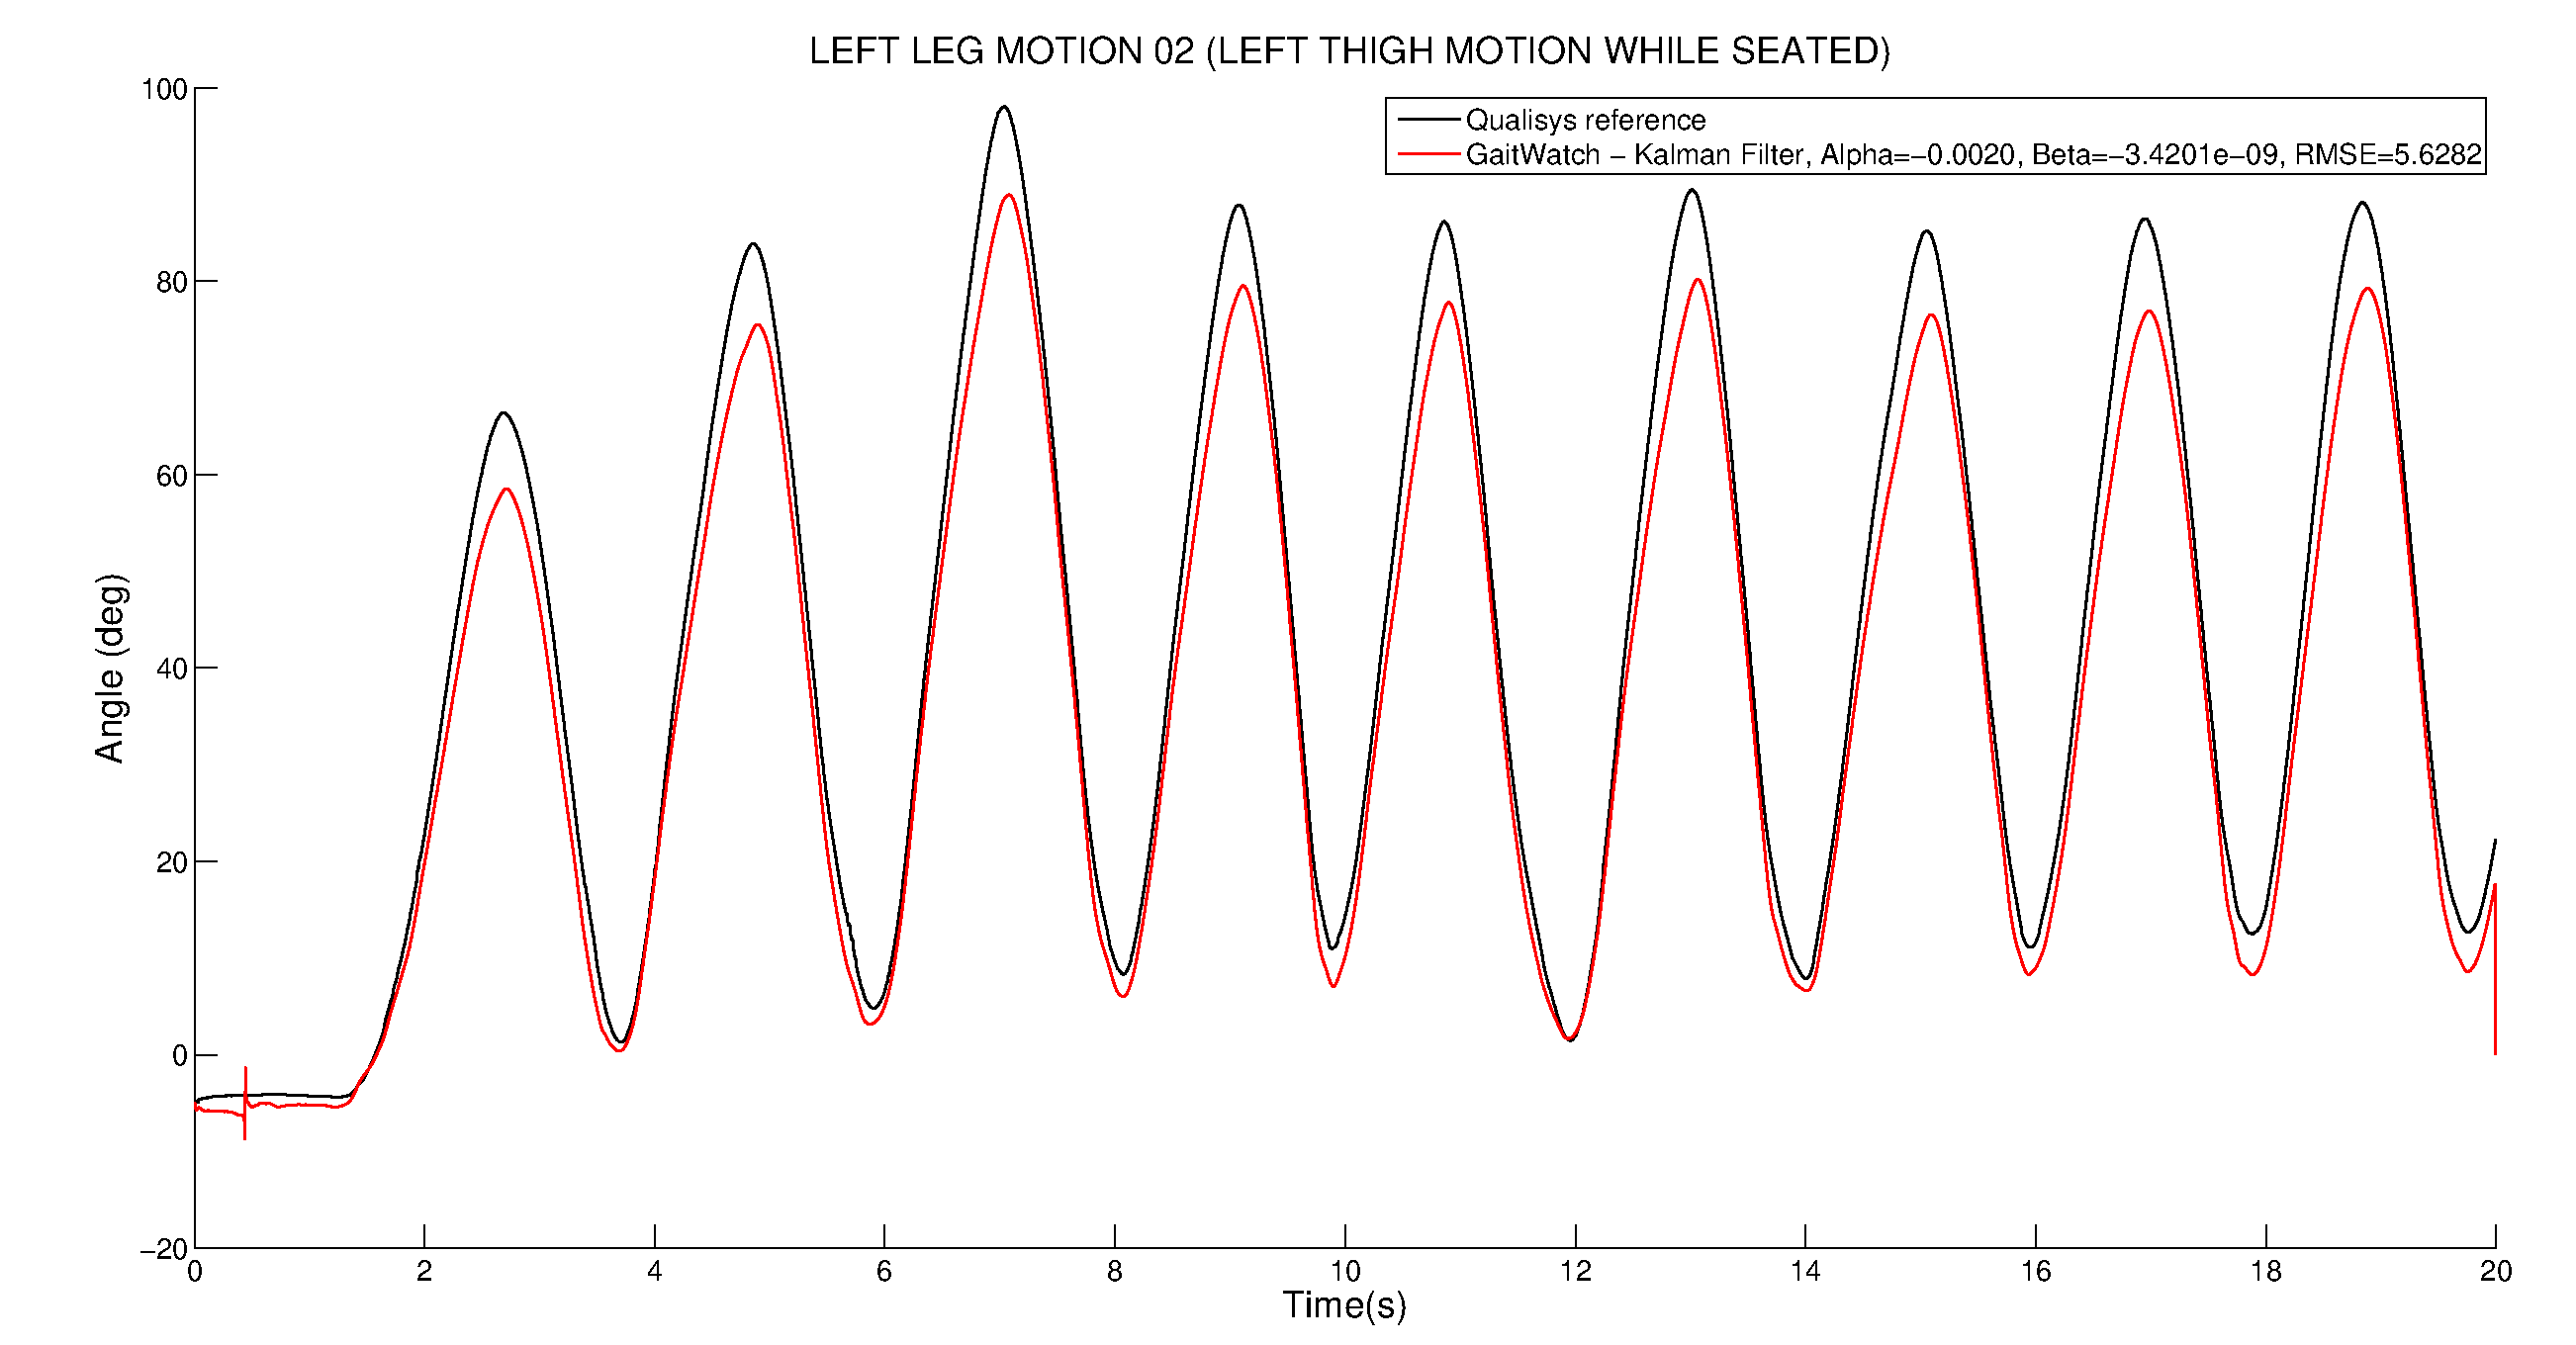
\includegraphics[width=1\textwidth]{figures/Left_leg_motion_02_thigh.eps}
\caption{Pitch angle while swinging left thigh. (GaitWatch vs. Qualisys).}
\label{fig:Left_leg_motion_02_thigh}
\end{figure}

\begin{figure}[H]
\centering
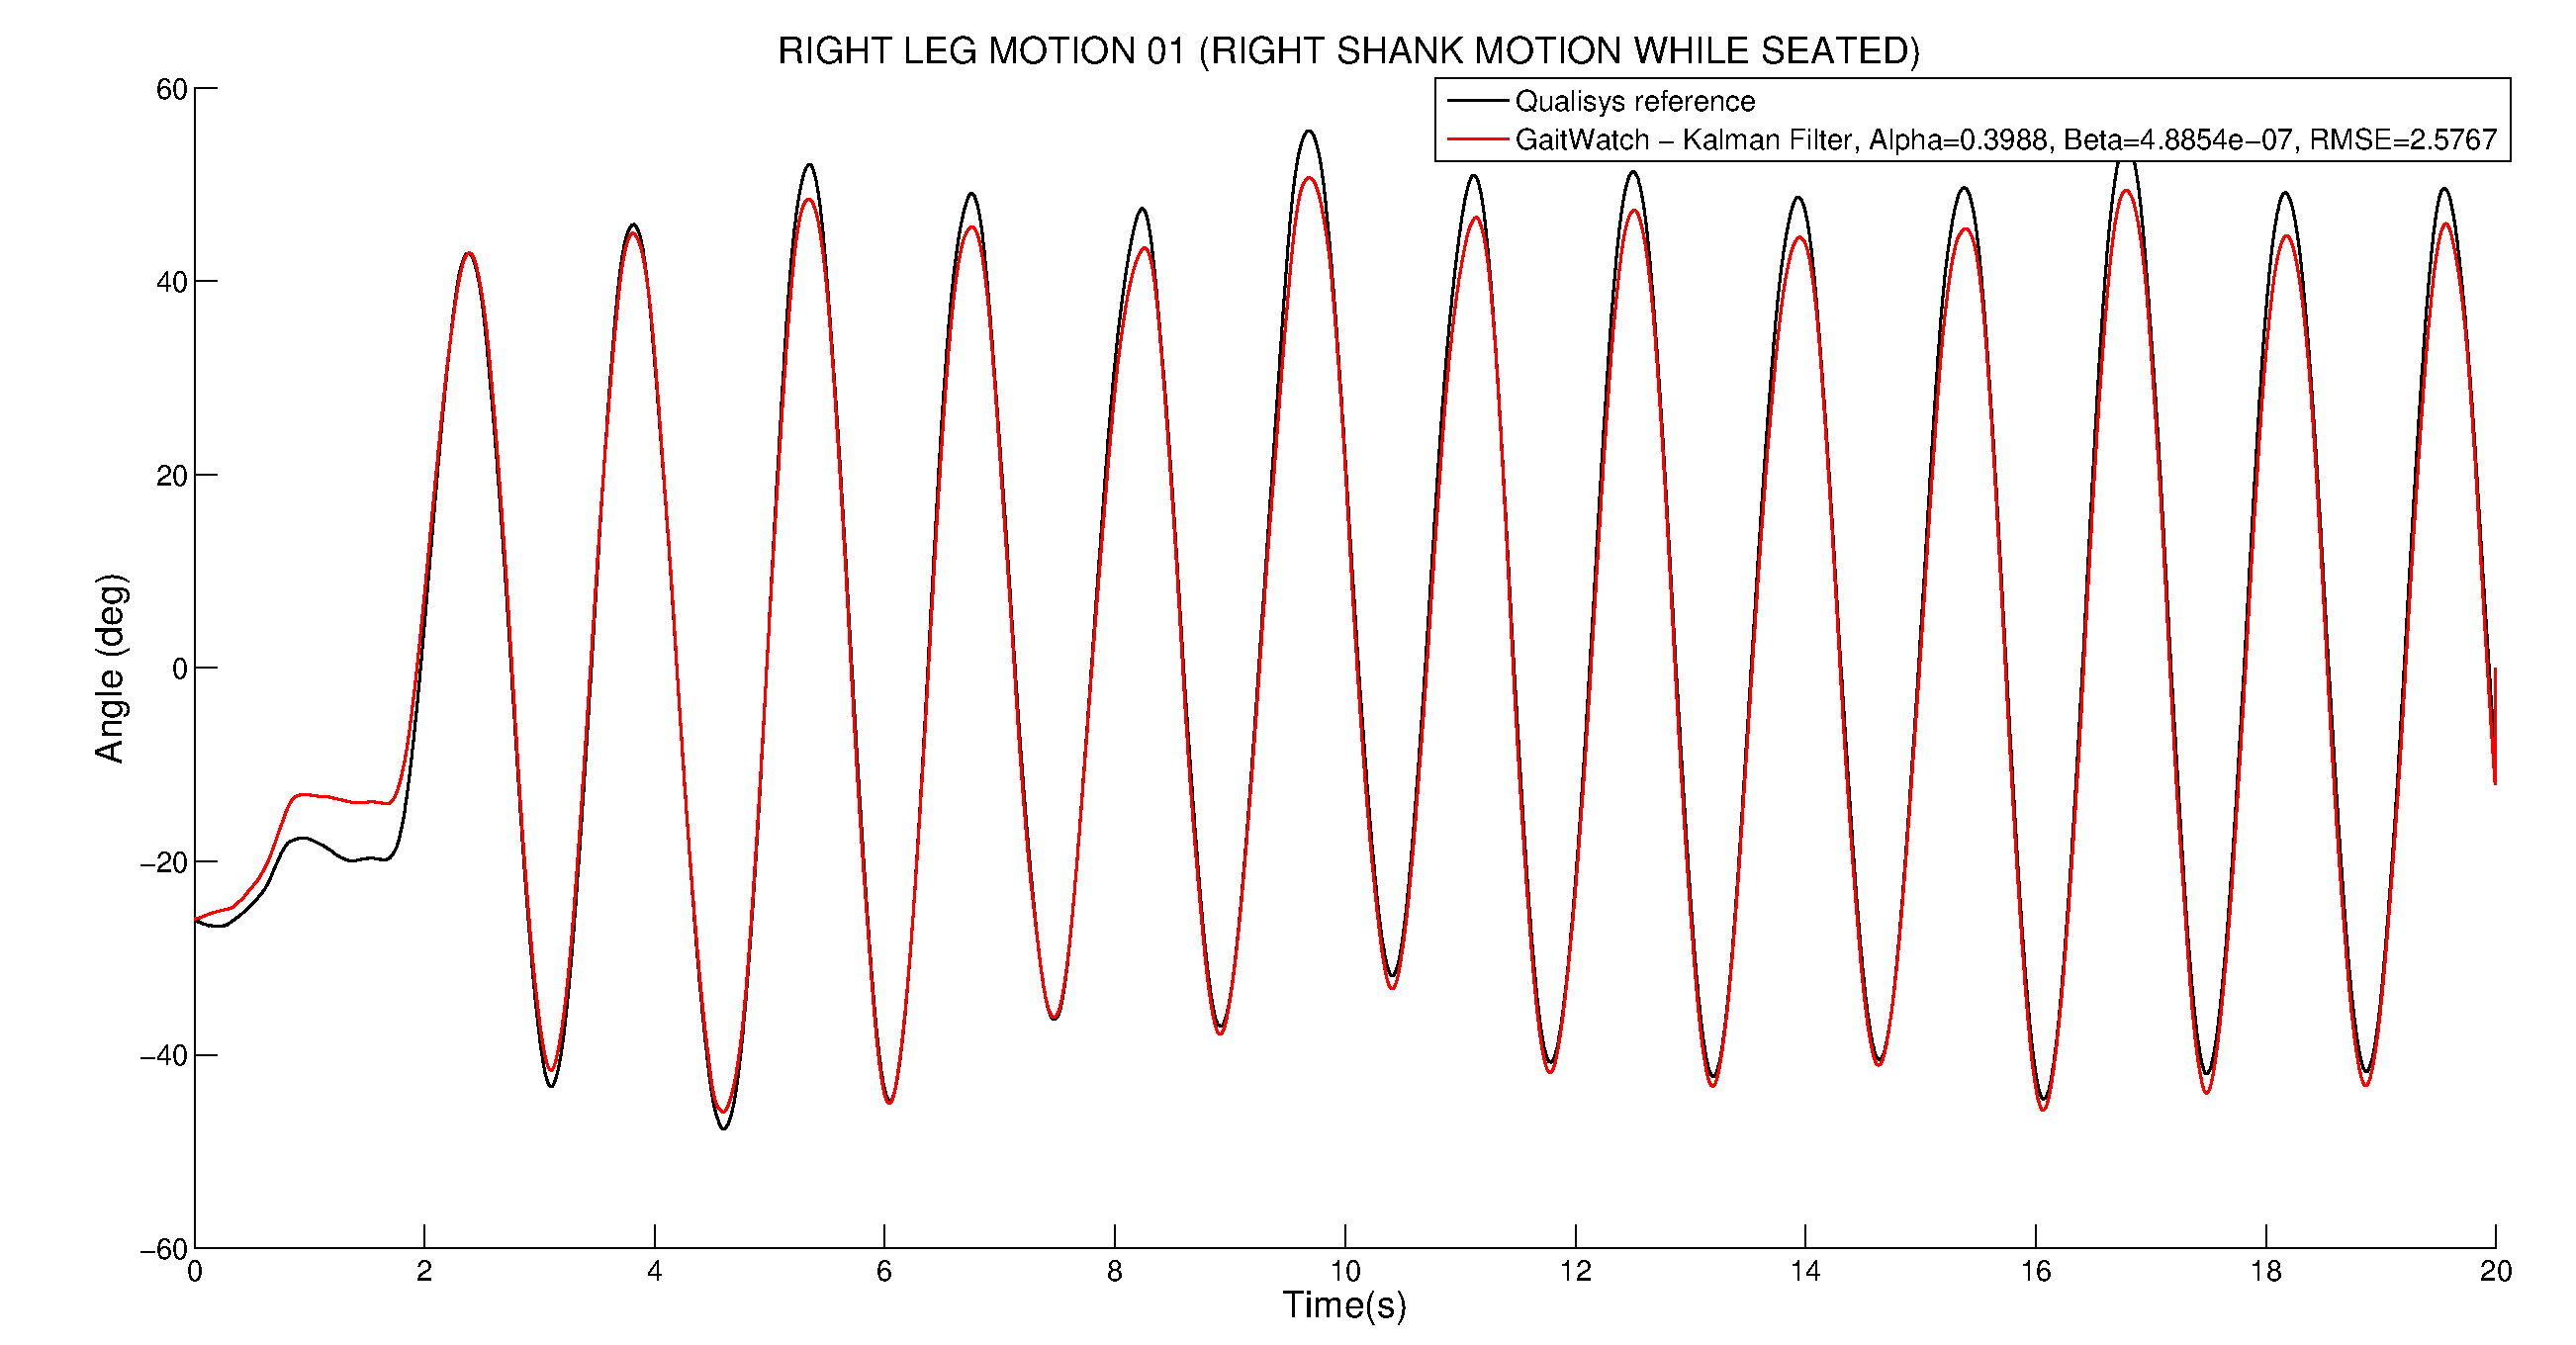
\includegraphics[width=1\textwidth]{figures/Right_leg_motion_01_shank.eps}
\caption{Pitch angle while swinging right shank. (GaitWatch vs. Qualisys).}
\label{fig:Right_leg_motion_01_shank}
\end{figure}

\begin{figure}[H]
\centering
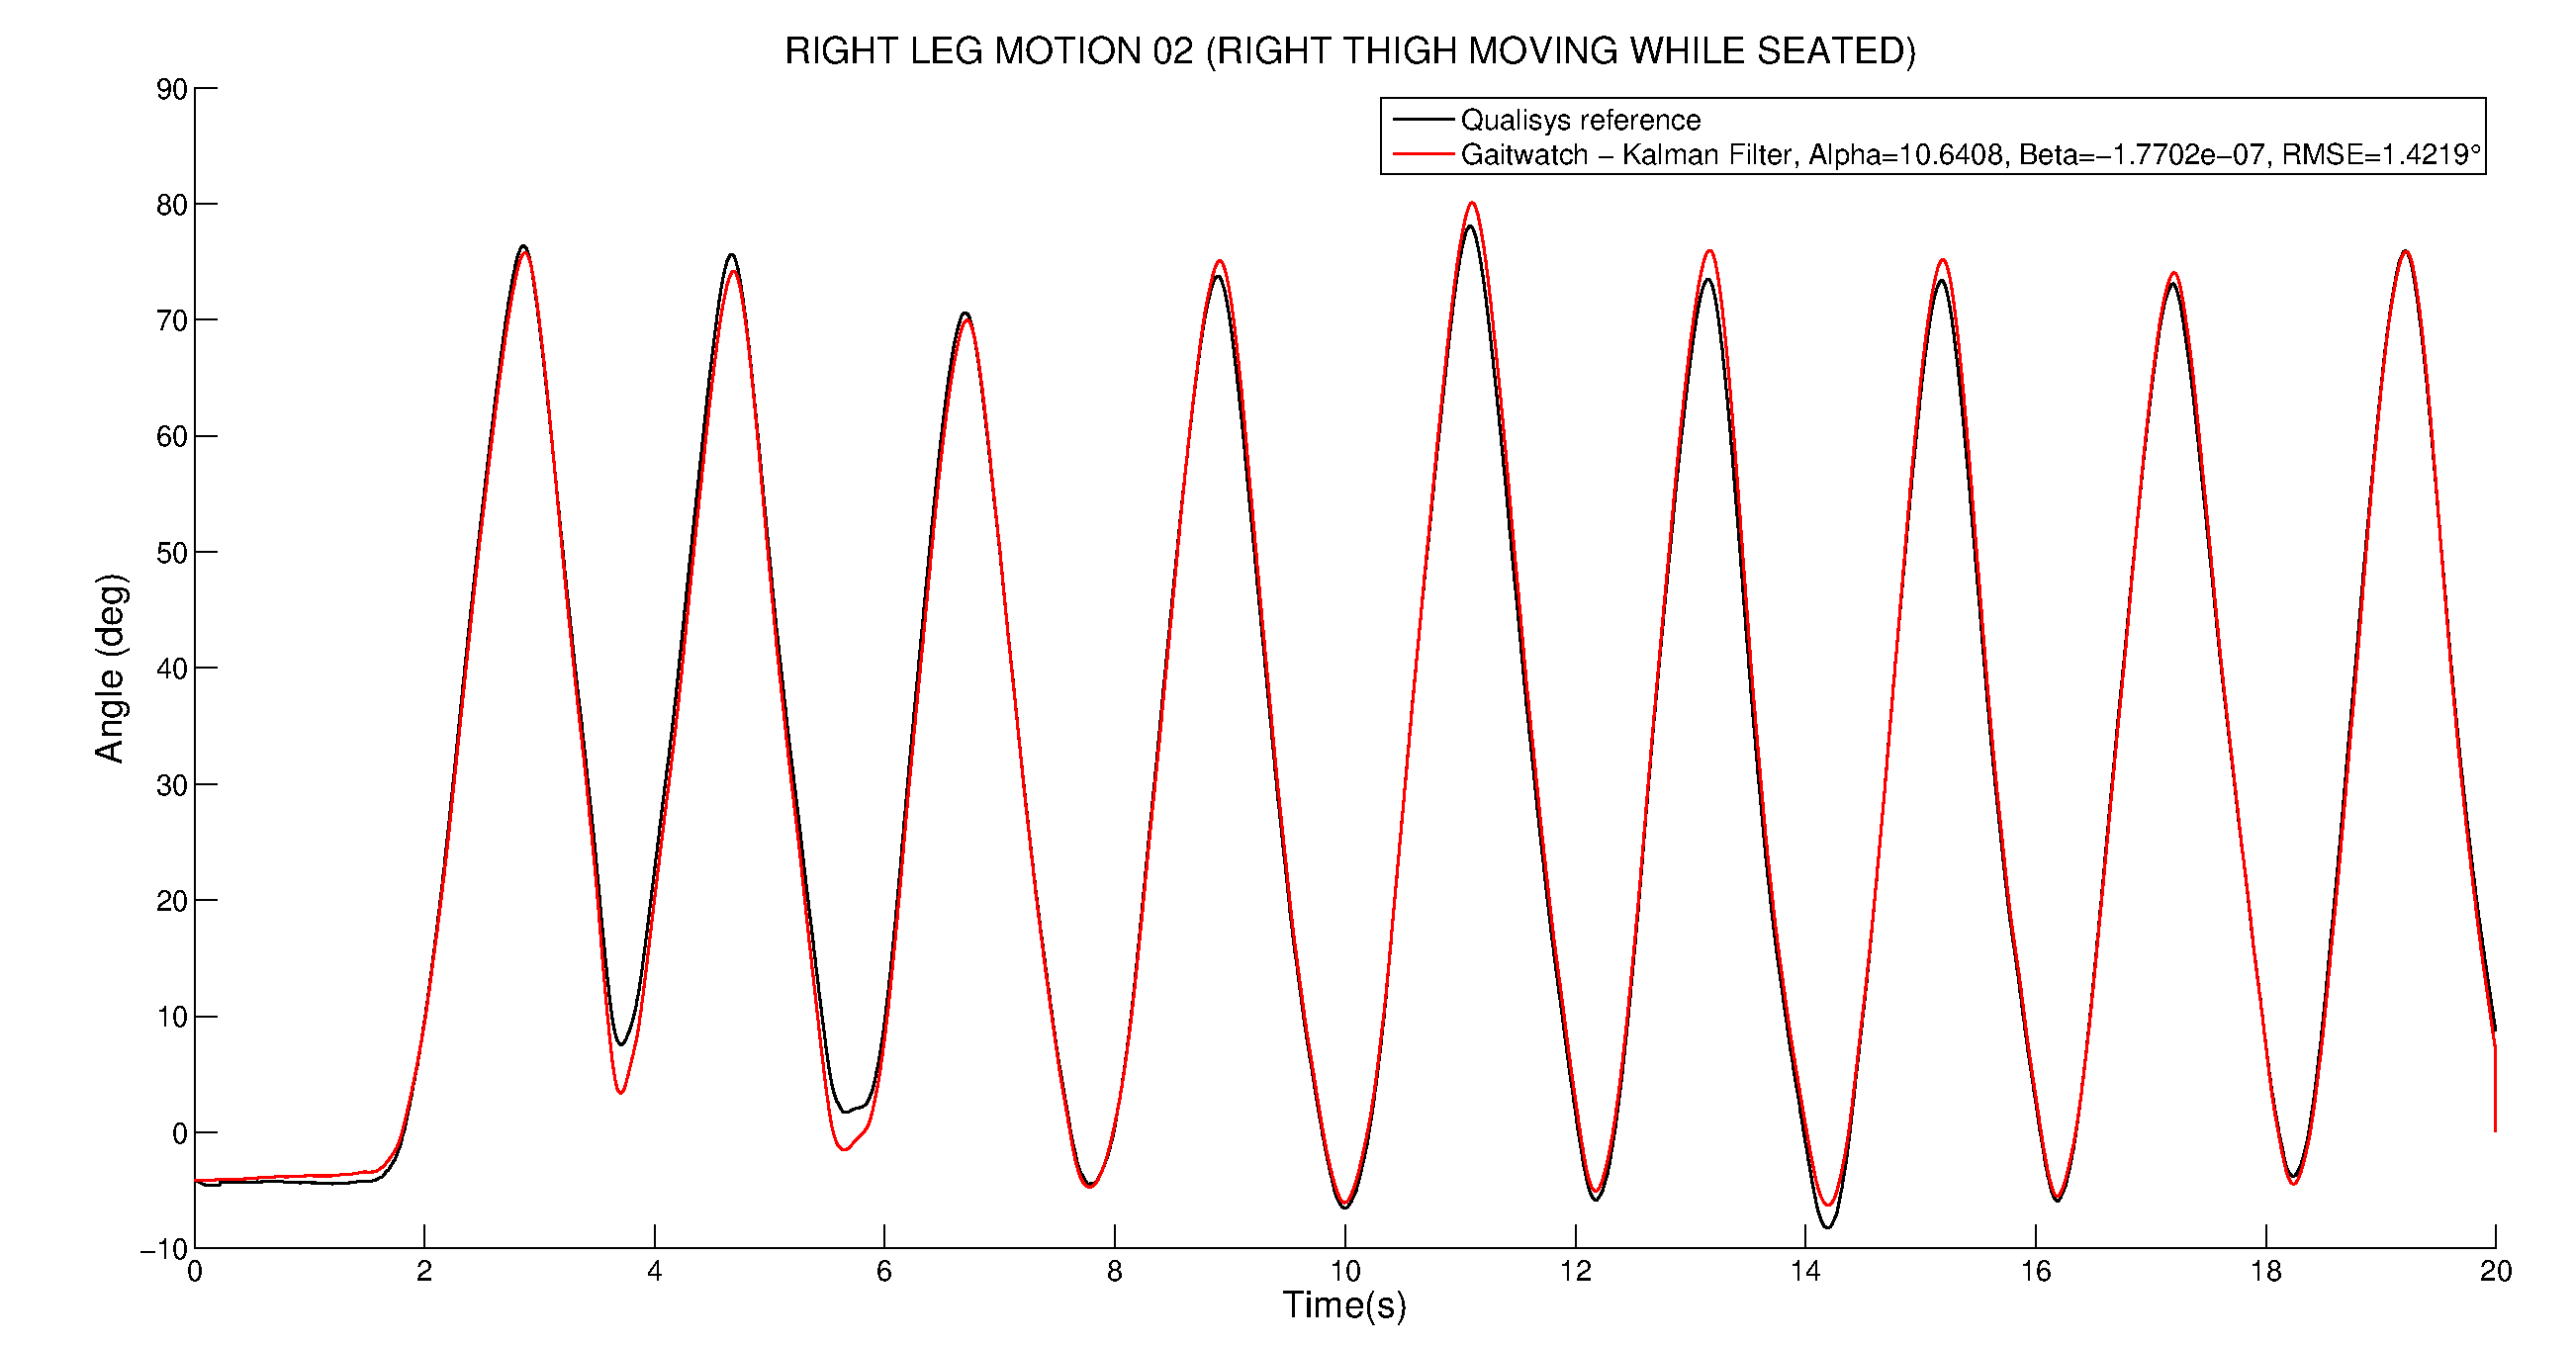
\includegraphics[width=1\textwidth]{figures/Right_leg_motion_02_thigh.eps}
\caption{Pitch angle while swinging right thigh. (GaitWatch vs. Qualisys).}
\label{fig:Right_leg_motion_02_thigh}
\end{figure}

\section{Freezing gait}

\begin{figure}[H]
\centering
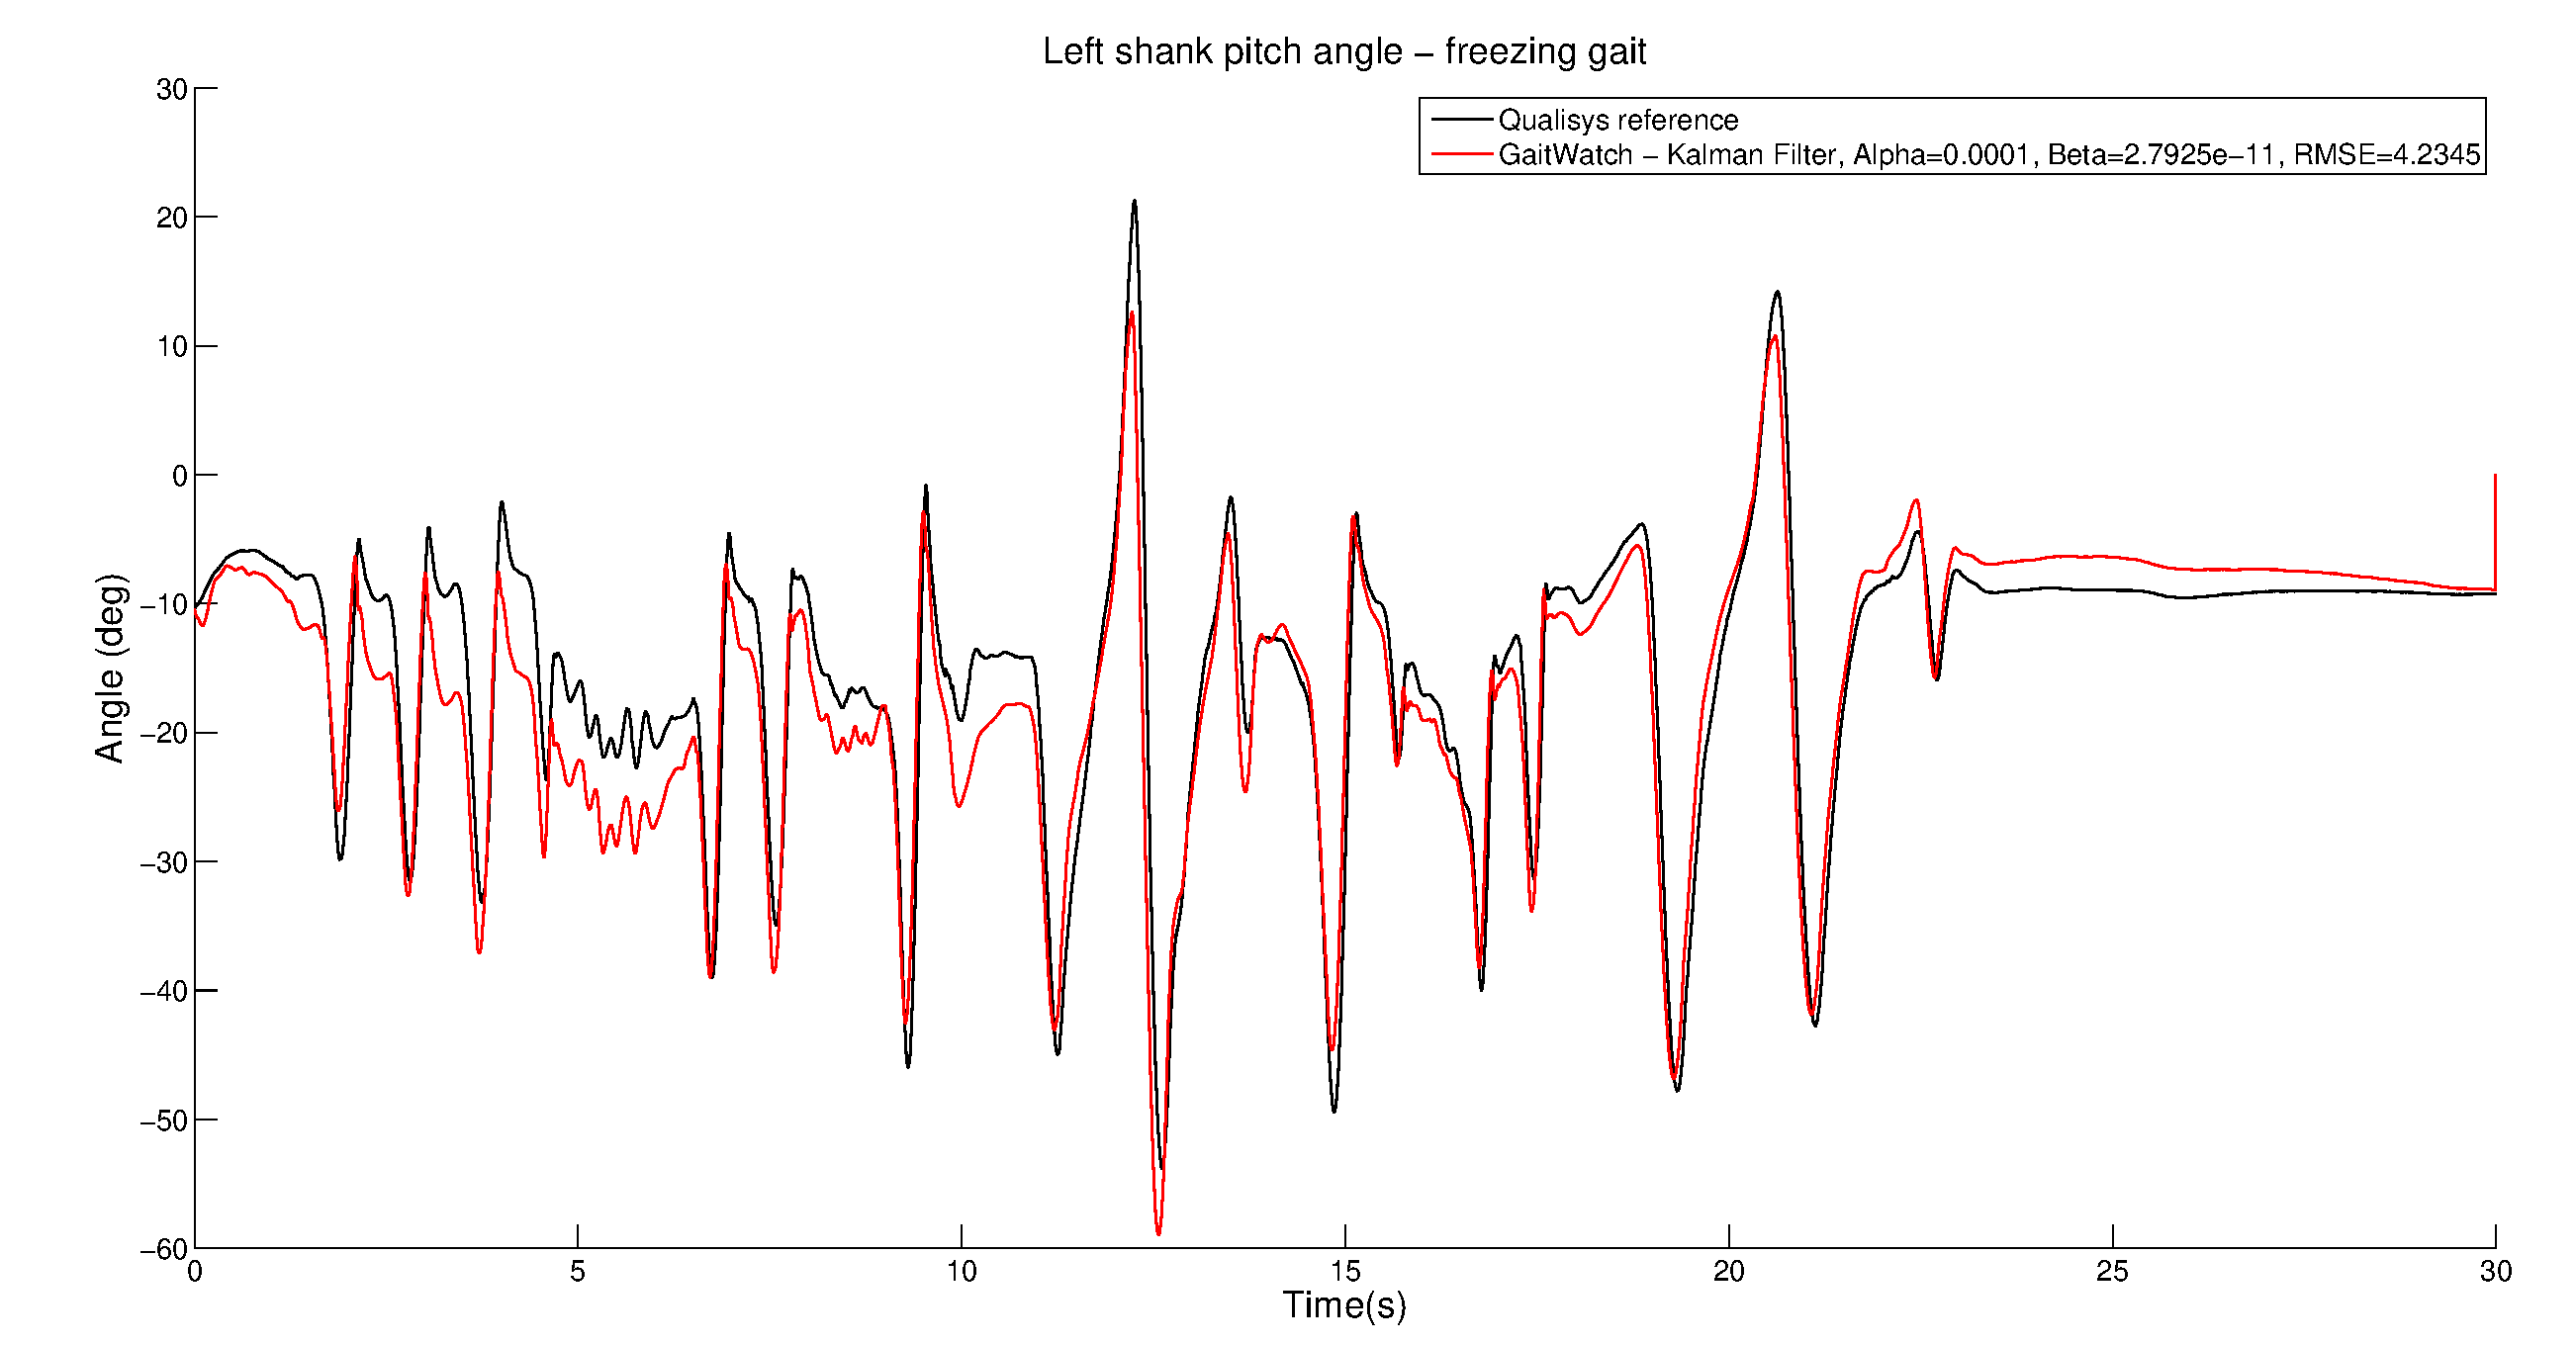
\includegraphics[width=1\textwidth]{figures/freezing_gait_left_shank.eps}
\caption{Left shank's pitch angle during freezing gait. (GaitWatch vs. Qualisys).}
\label{fig:freezing_gait_left_shank}
\end{figure}

\begin{figure}[H]
\centering
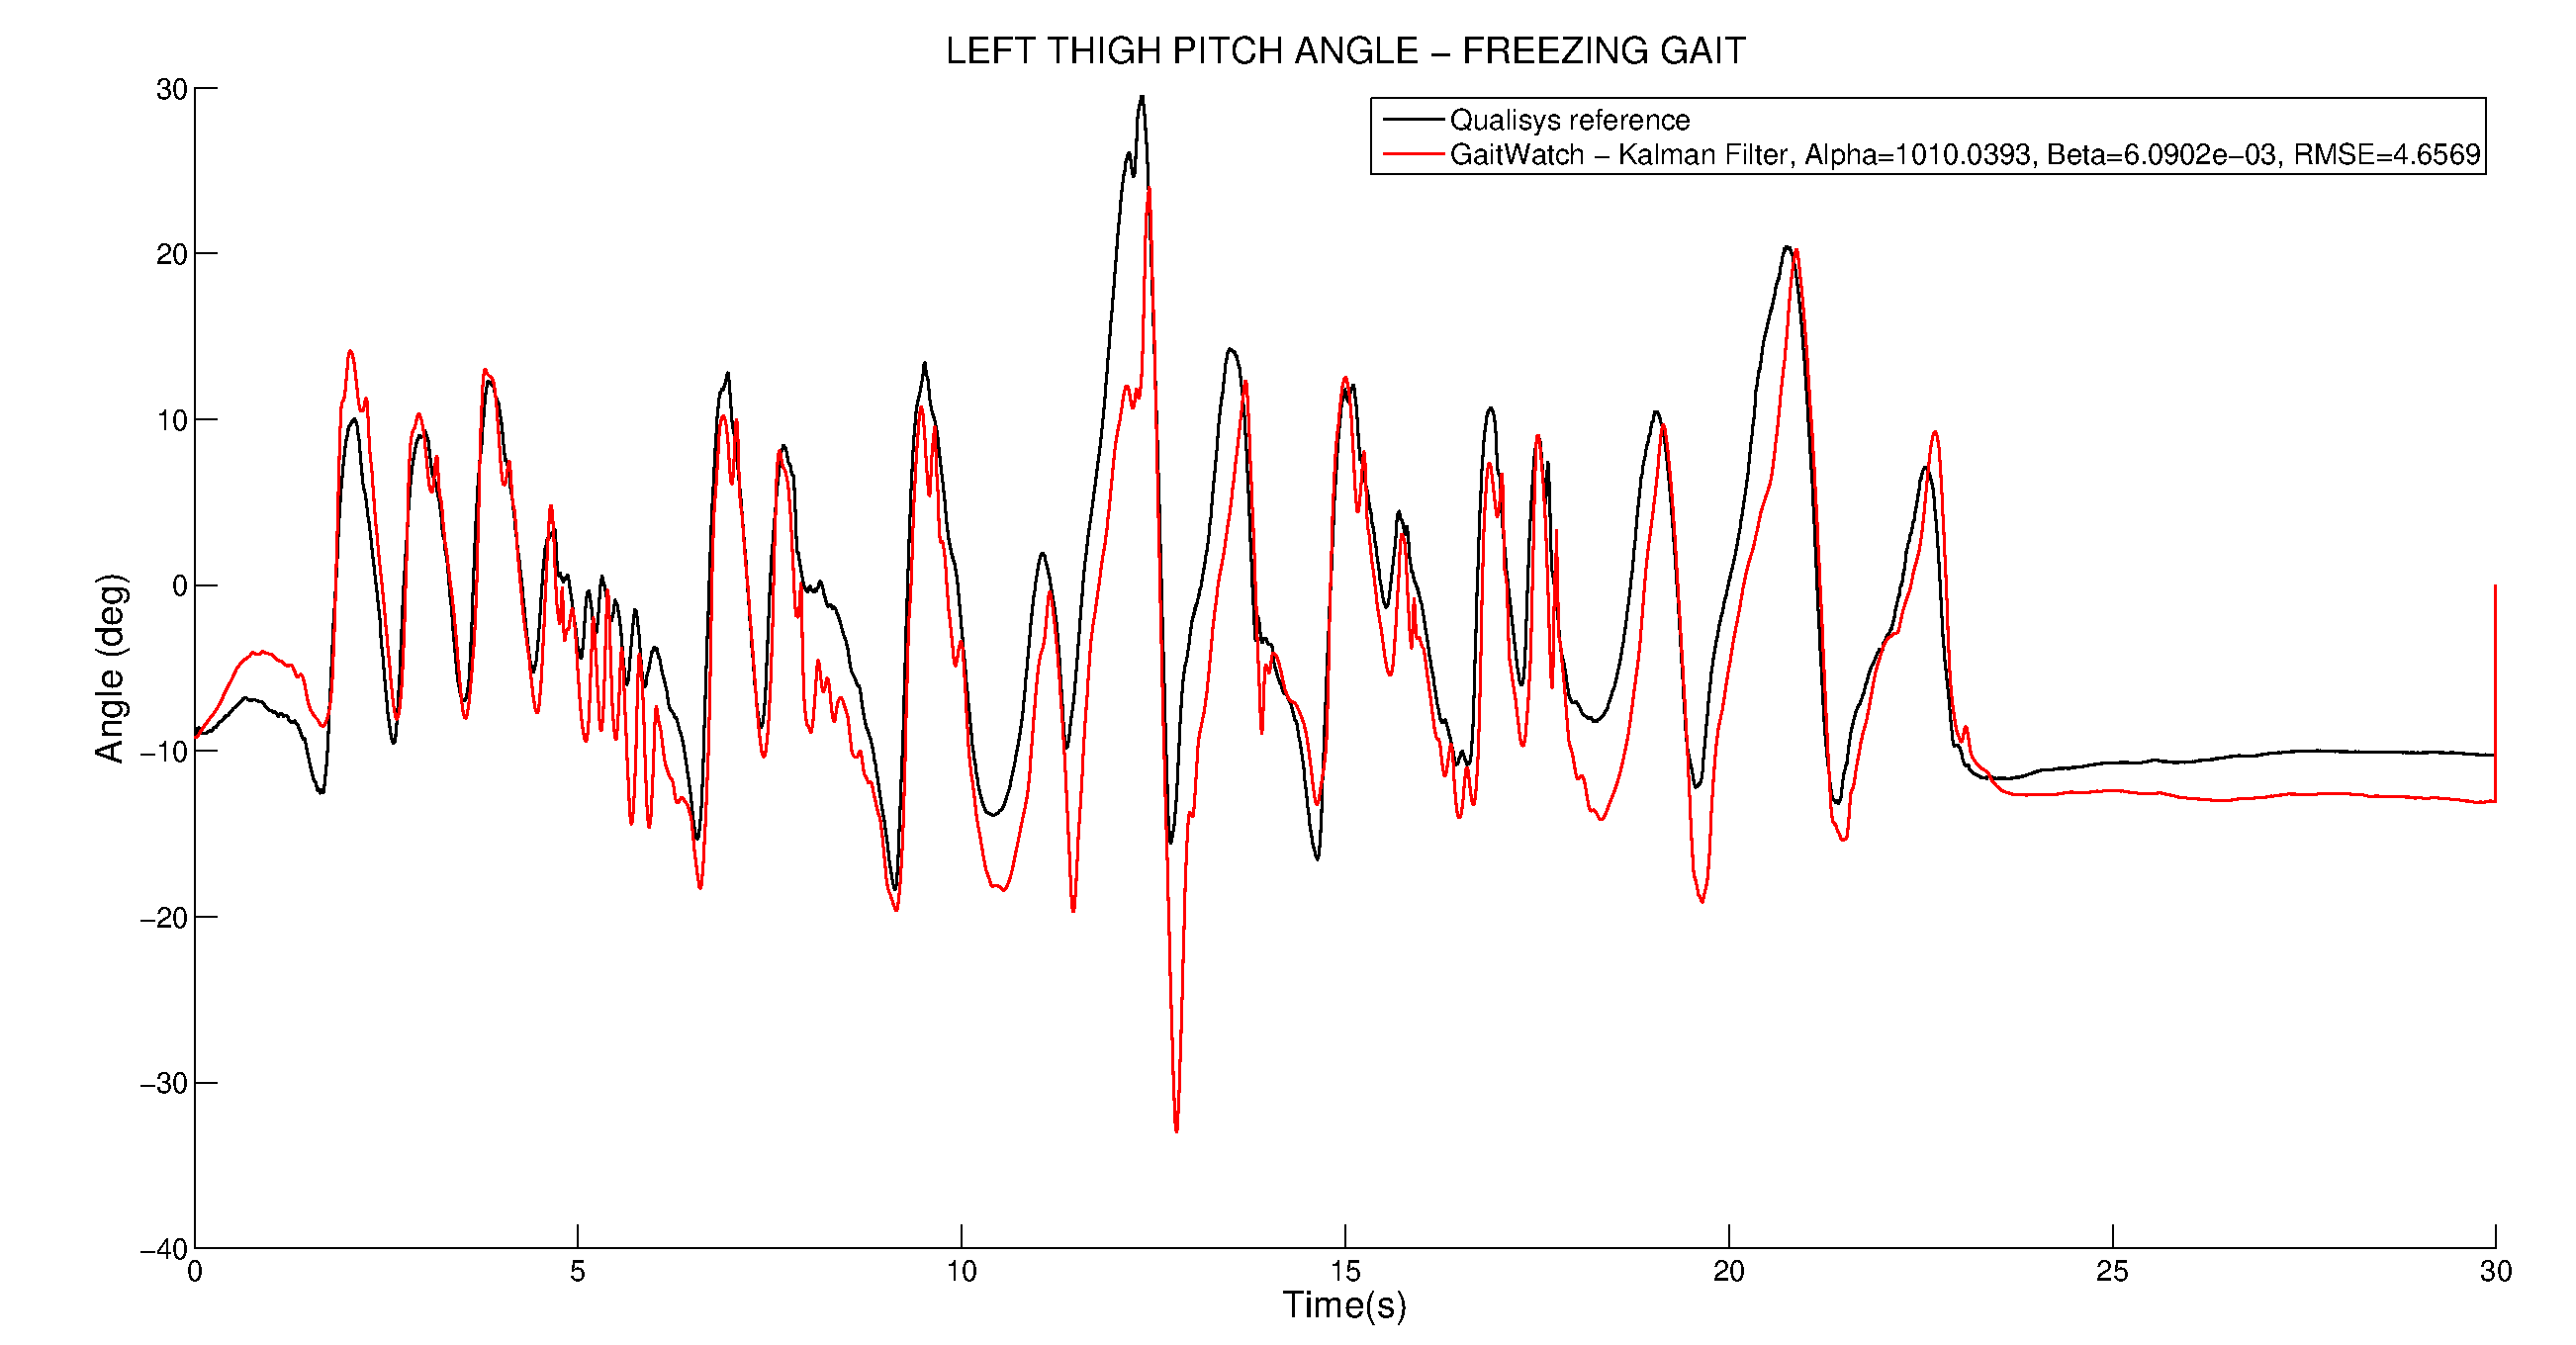
\includegraphics[width=1\textwidth]{figures/freezing_gait_left_thigh.eps}
\caption{Left thigh's pitch angle during freezing gait. (GaitWatch vs. Qualisys).}
\label{fig:freezing_gait_left_thigh}
\end{figure}

\begin{figure}[H]
\centering
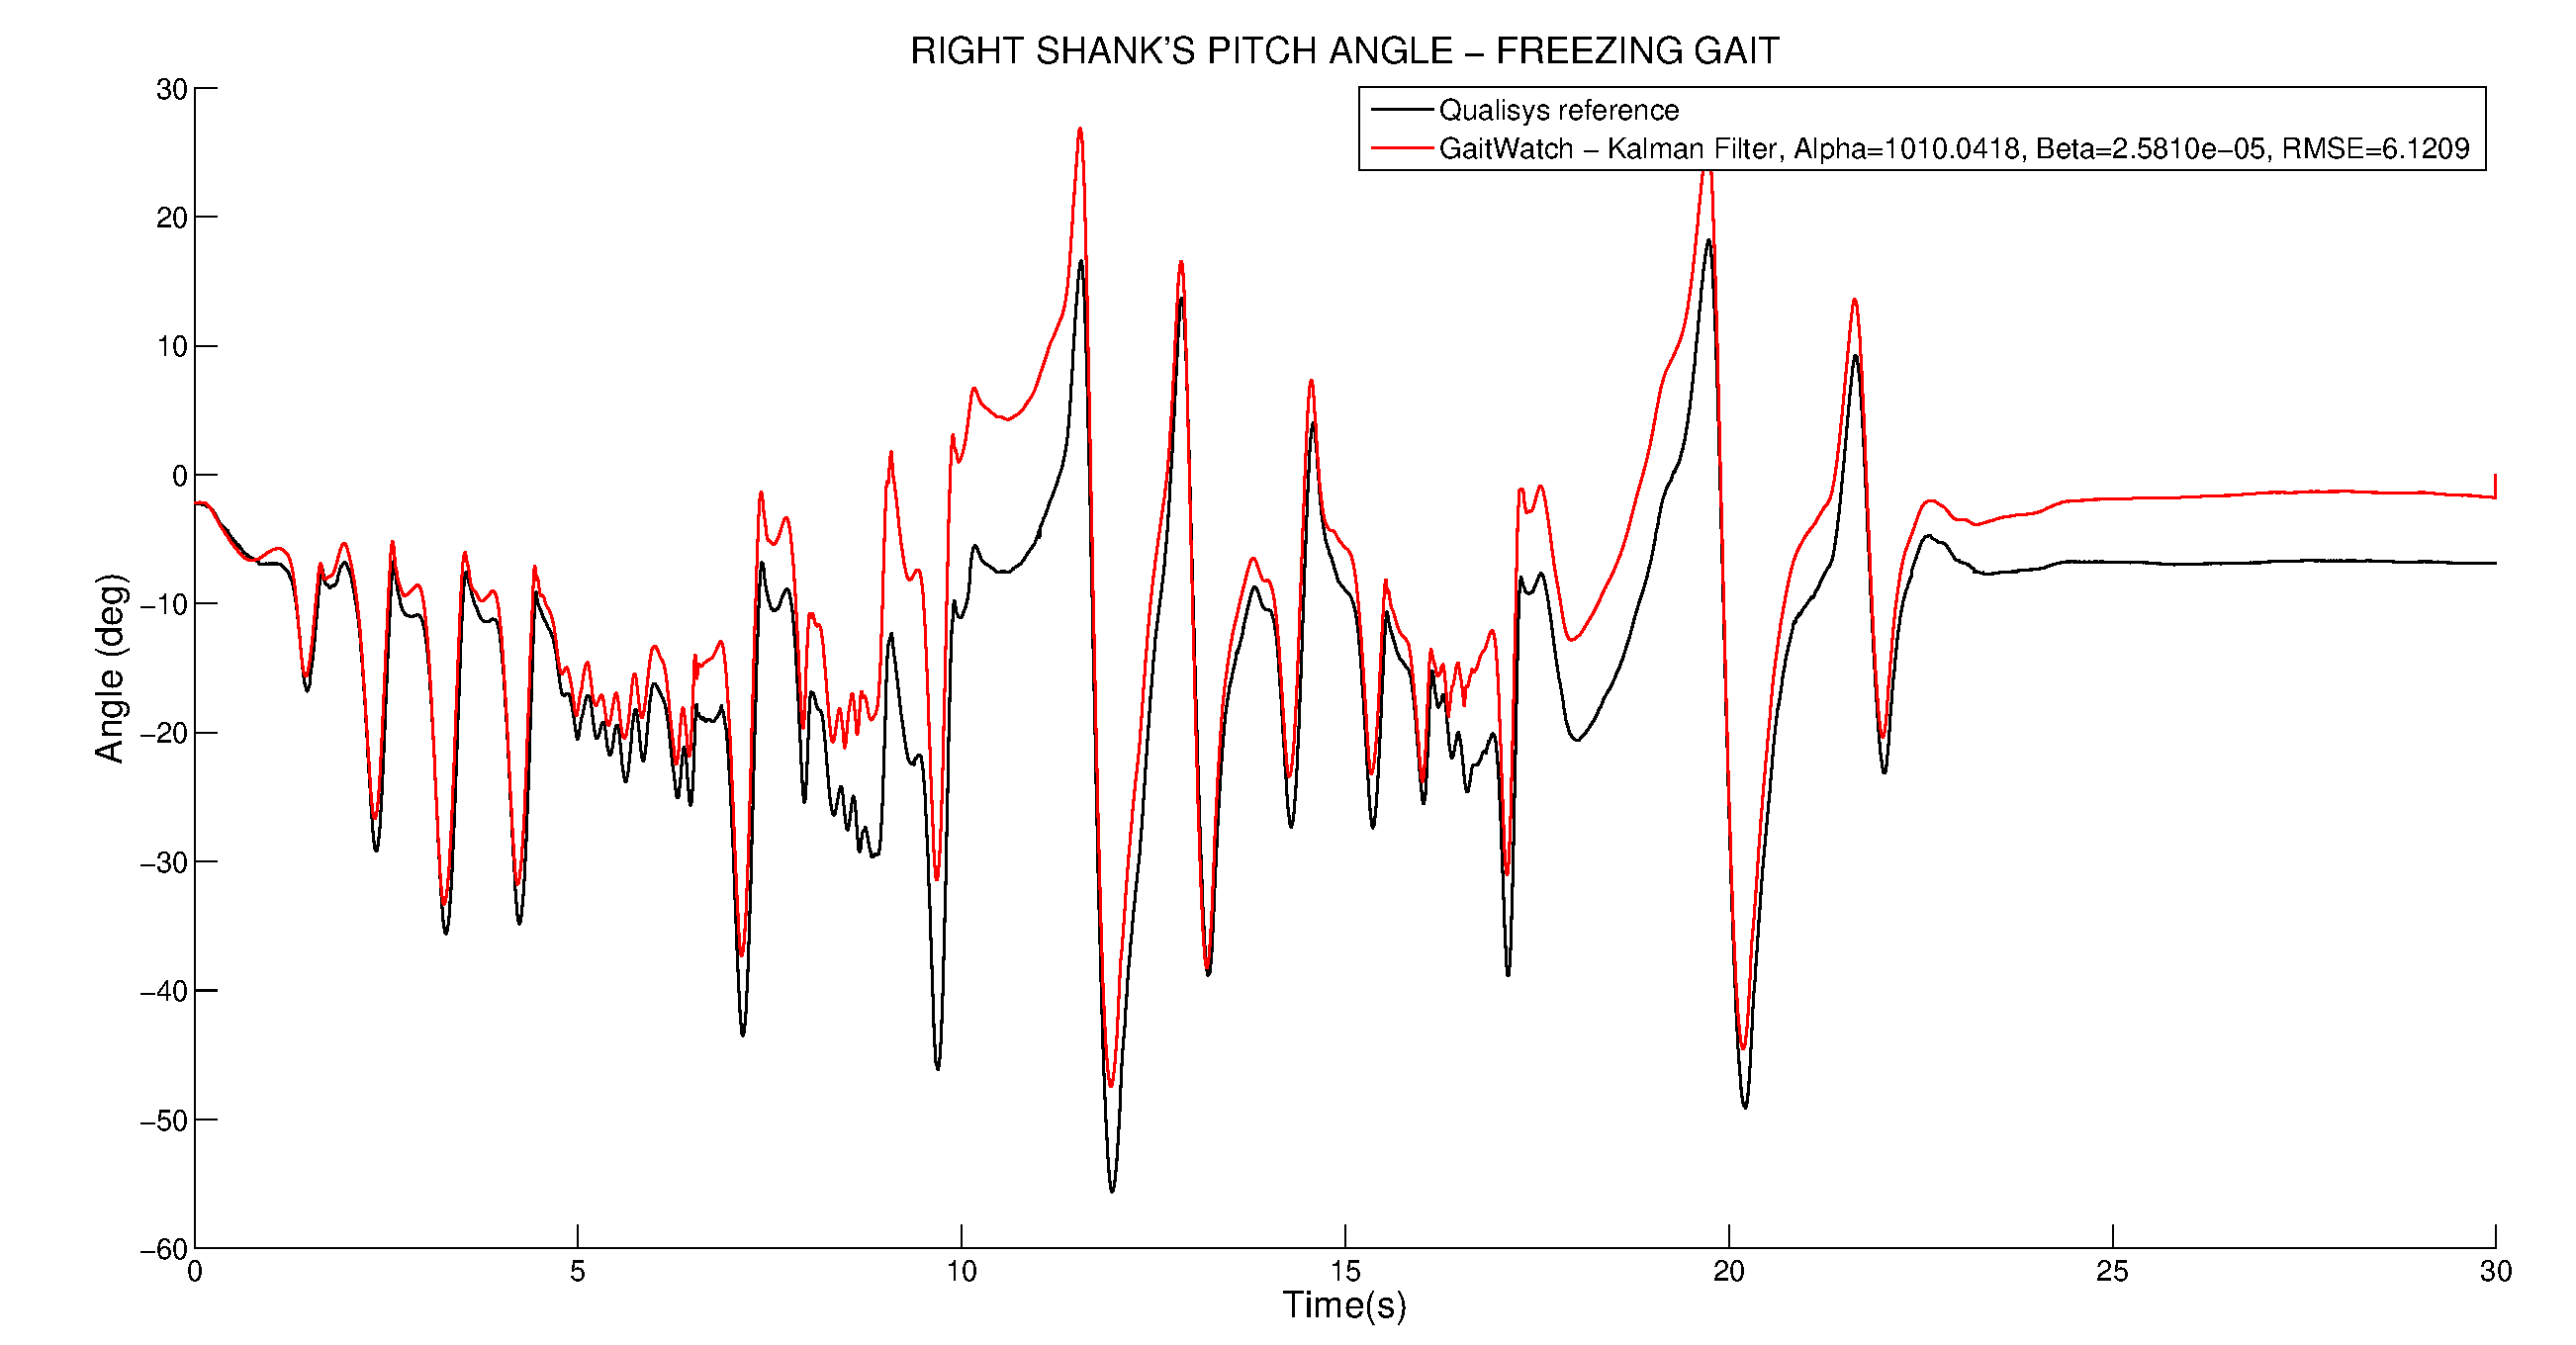
\includegraphics[width=1\textwidth]{figures/freezing_gait_right_shank.eps}
\caption{Right shank's pitch angle during freezing gait. (GaitWatch vs. Qualisys).}
\label{fig:freezing_gait_right_shank}
\end{figure}

\begin{figure}[H]
\centering
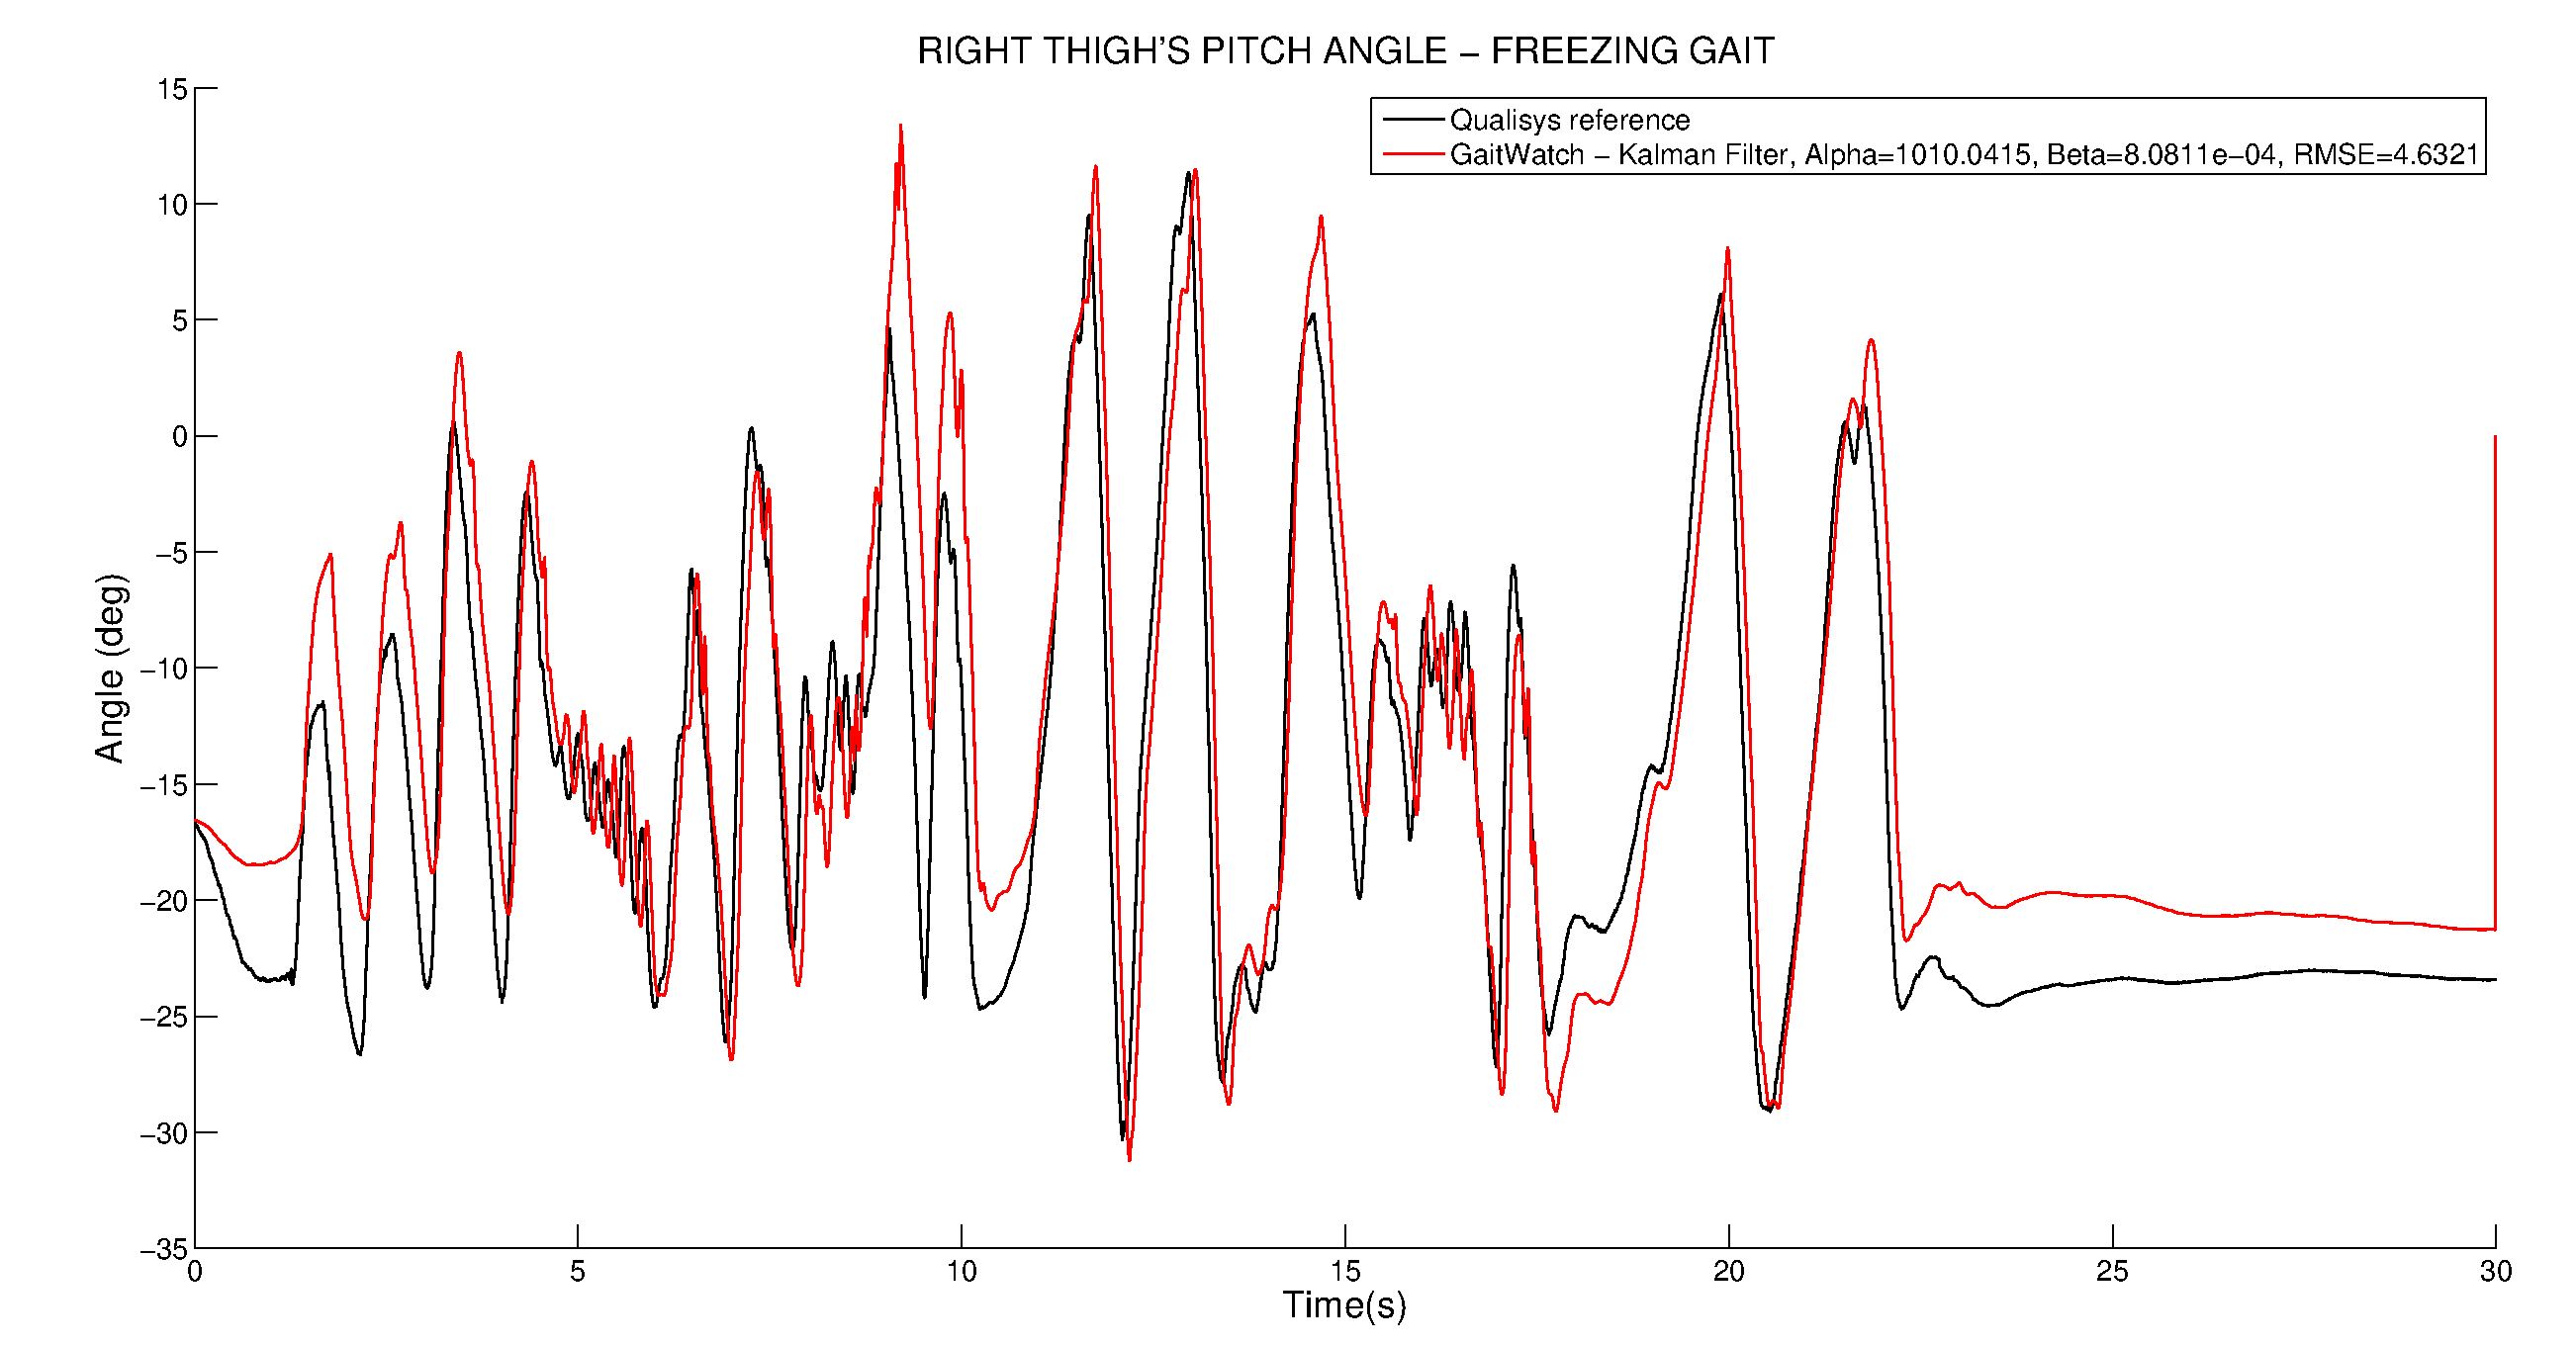
\includegraphics[width=1\textwidth]{figures/freezing_gait_right_thigh.eps}
\caption{Right thigh's pitch angle during freezing gait. (GaitWatch vs. Qualisys).}
\label{fig:freezing_gait_right_thigh}
\end{figure}

\section{Normal gait}

\begin{figure}[H]
\centering
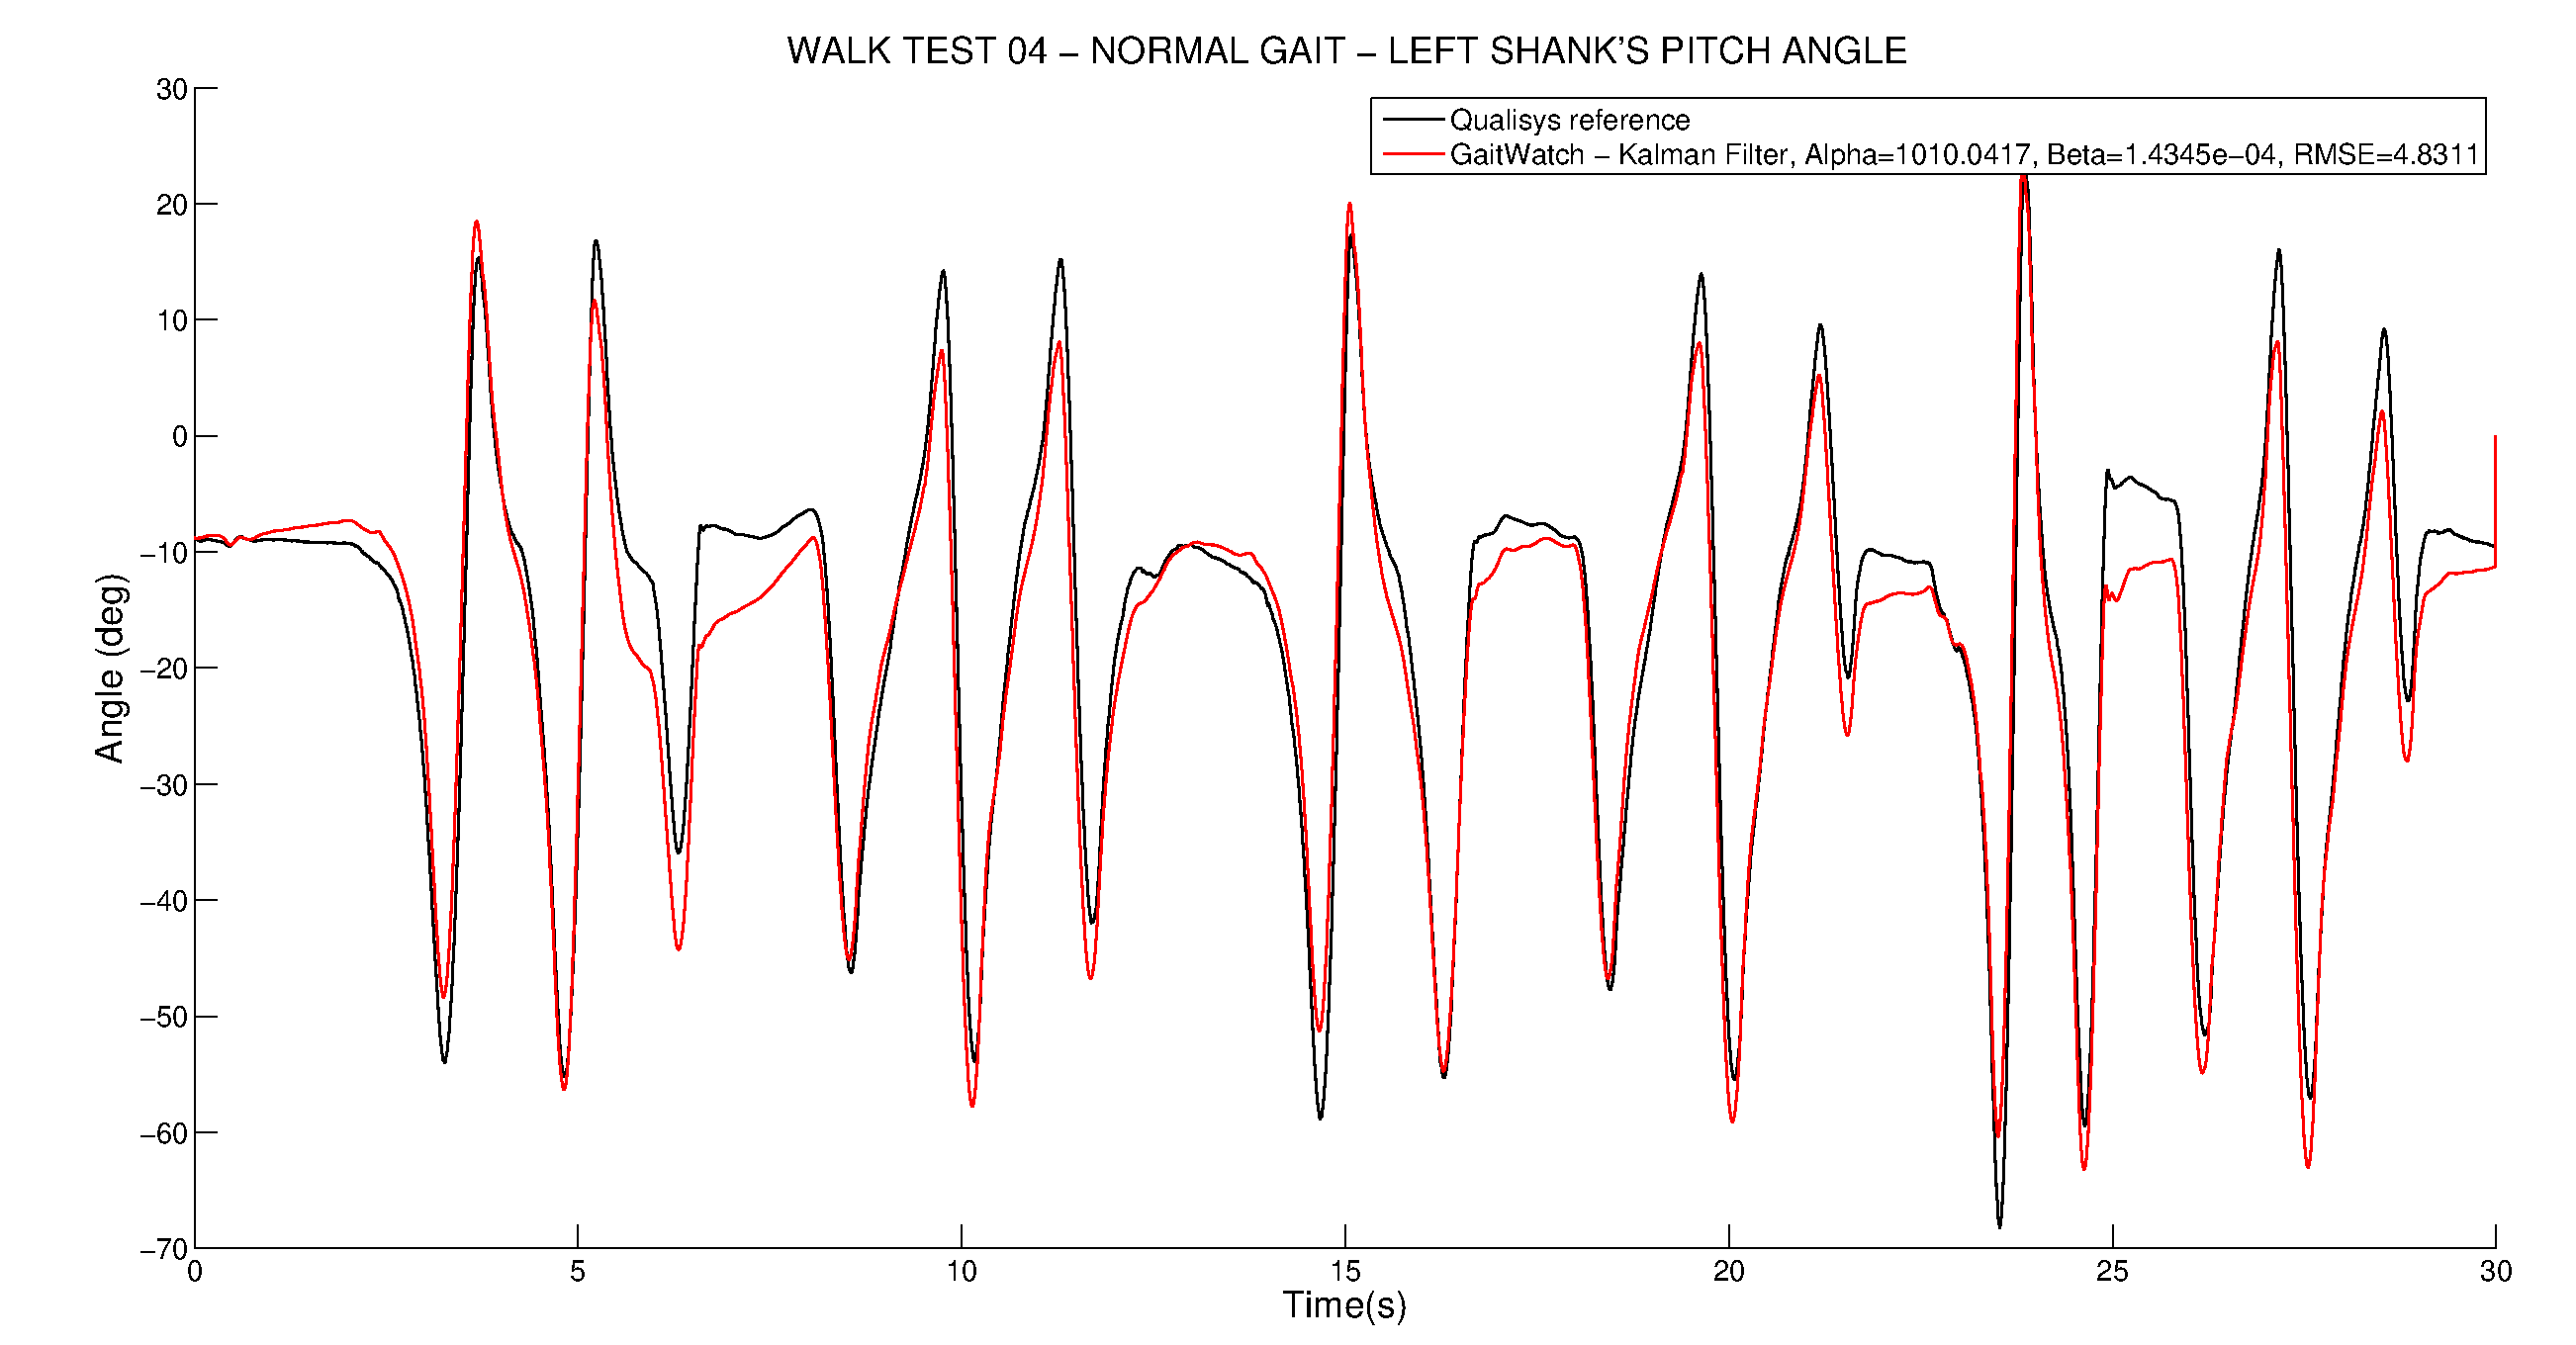
\includegraphics[width=1\textwidth]{figures/Walking_04_left_shank.eps}
\caption{Left shank's pitch angle during normal gait. (GaitWatch vs. Qualisys).}
\label{fig:Walking_04_left_shank}
\end{figure}

\begin{figure}[H]
\centering
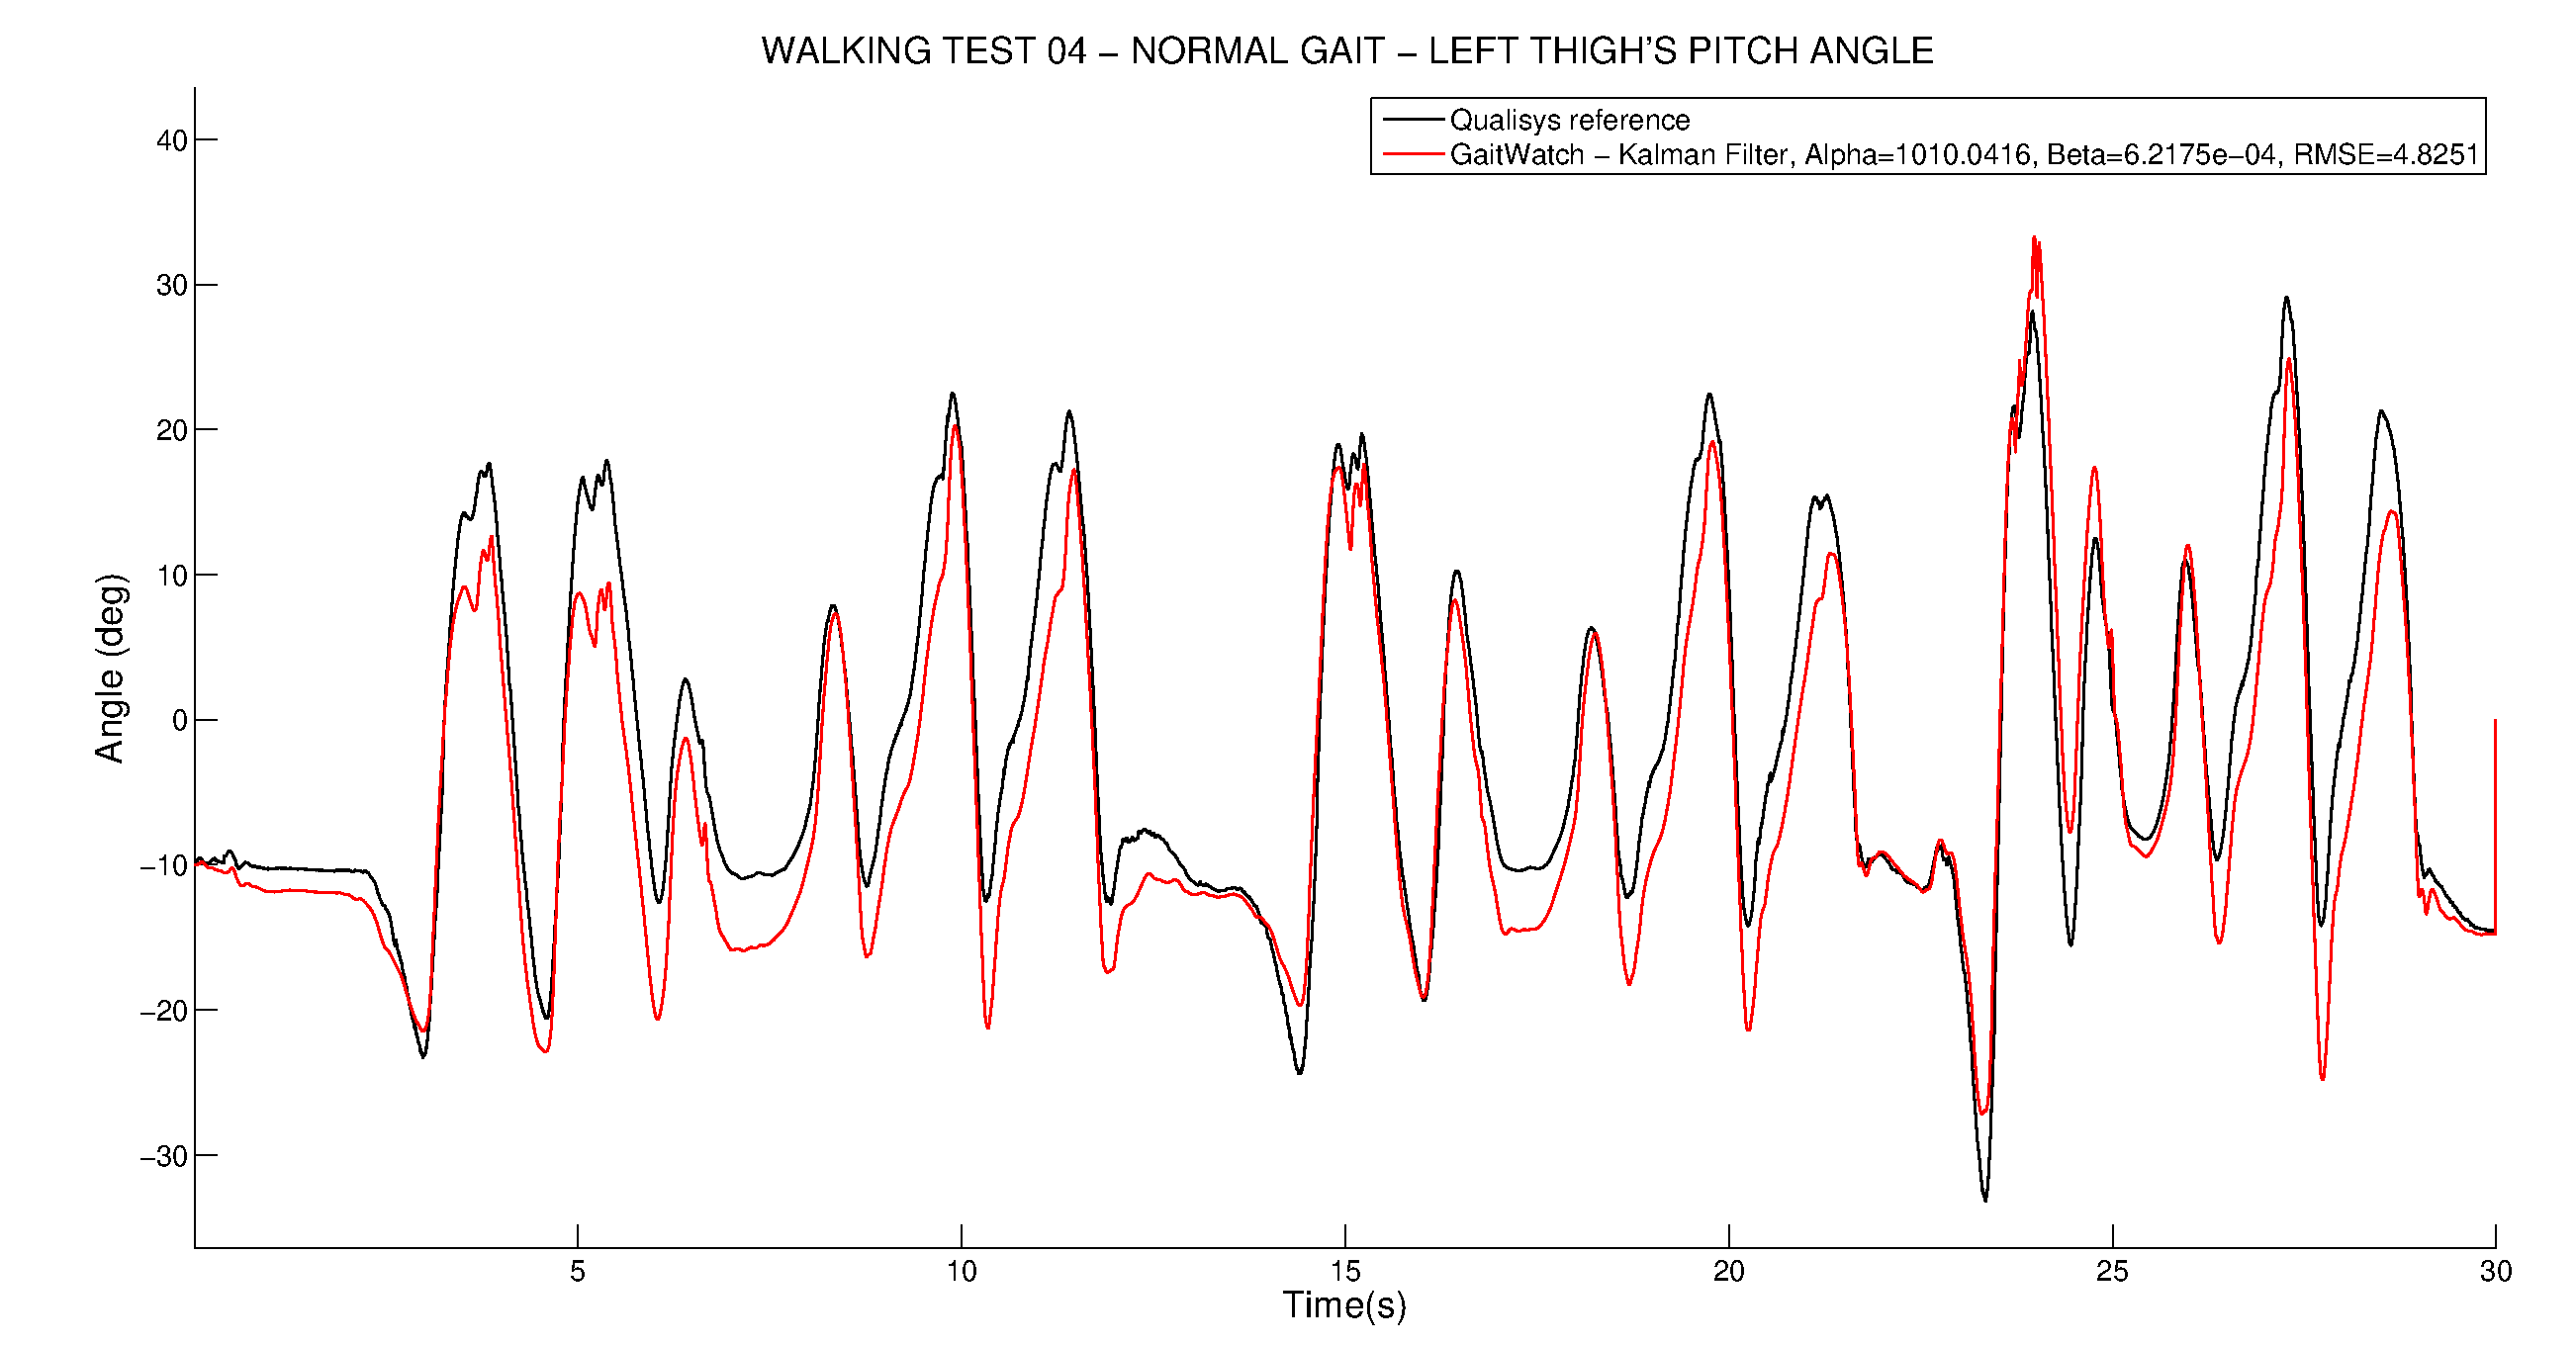
\includegraphics[width=1\textwidth]{figures/Walking_04_left_thigh.eps}
\caption{Left thigh's pitch angle during normal gait. (GaitWatch vs. Qualisys).}
\label{fig:Walking_04_left_thigh}
\end{figure}

\begin{figure}[H]
\centering
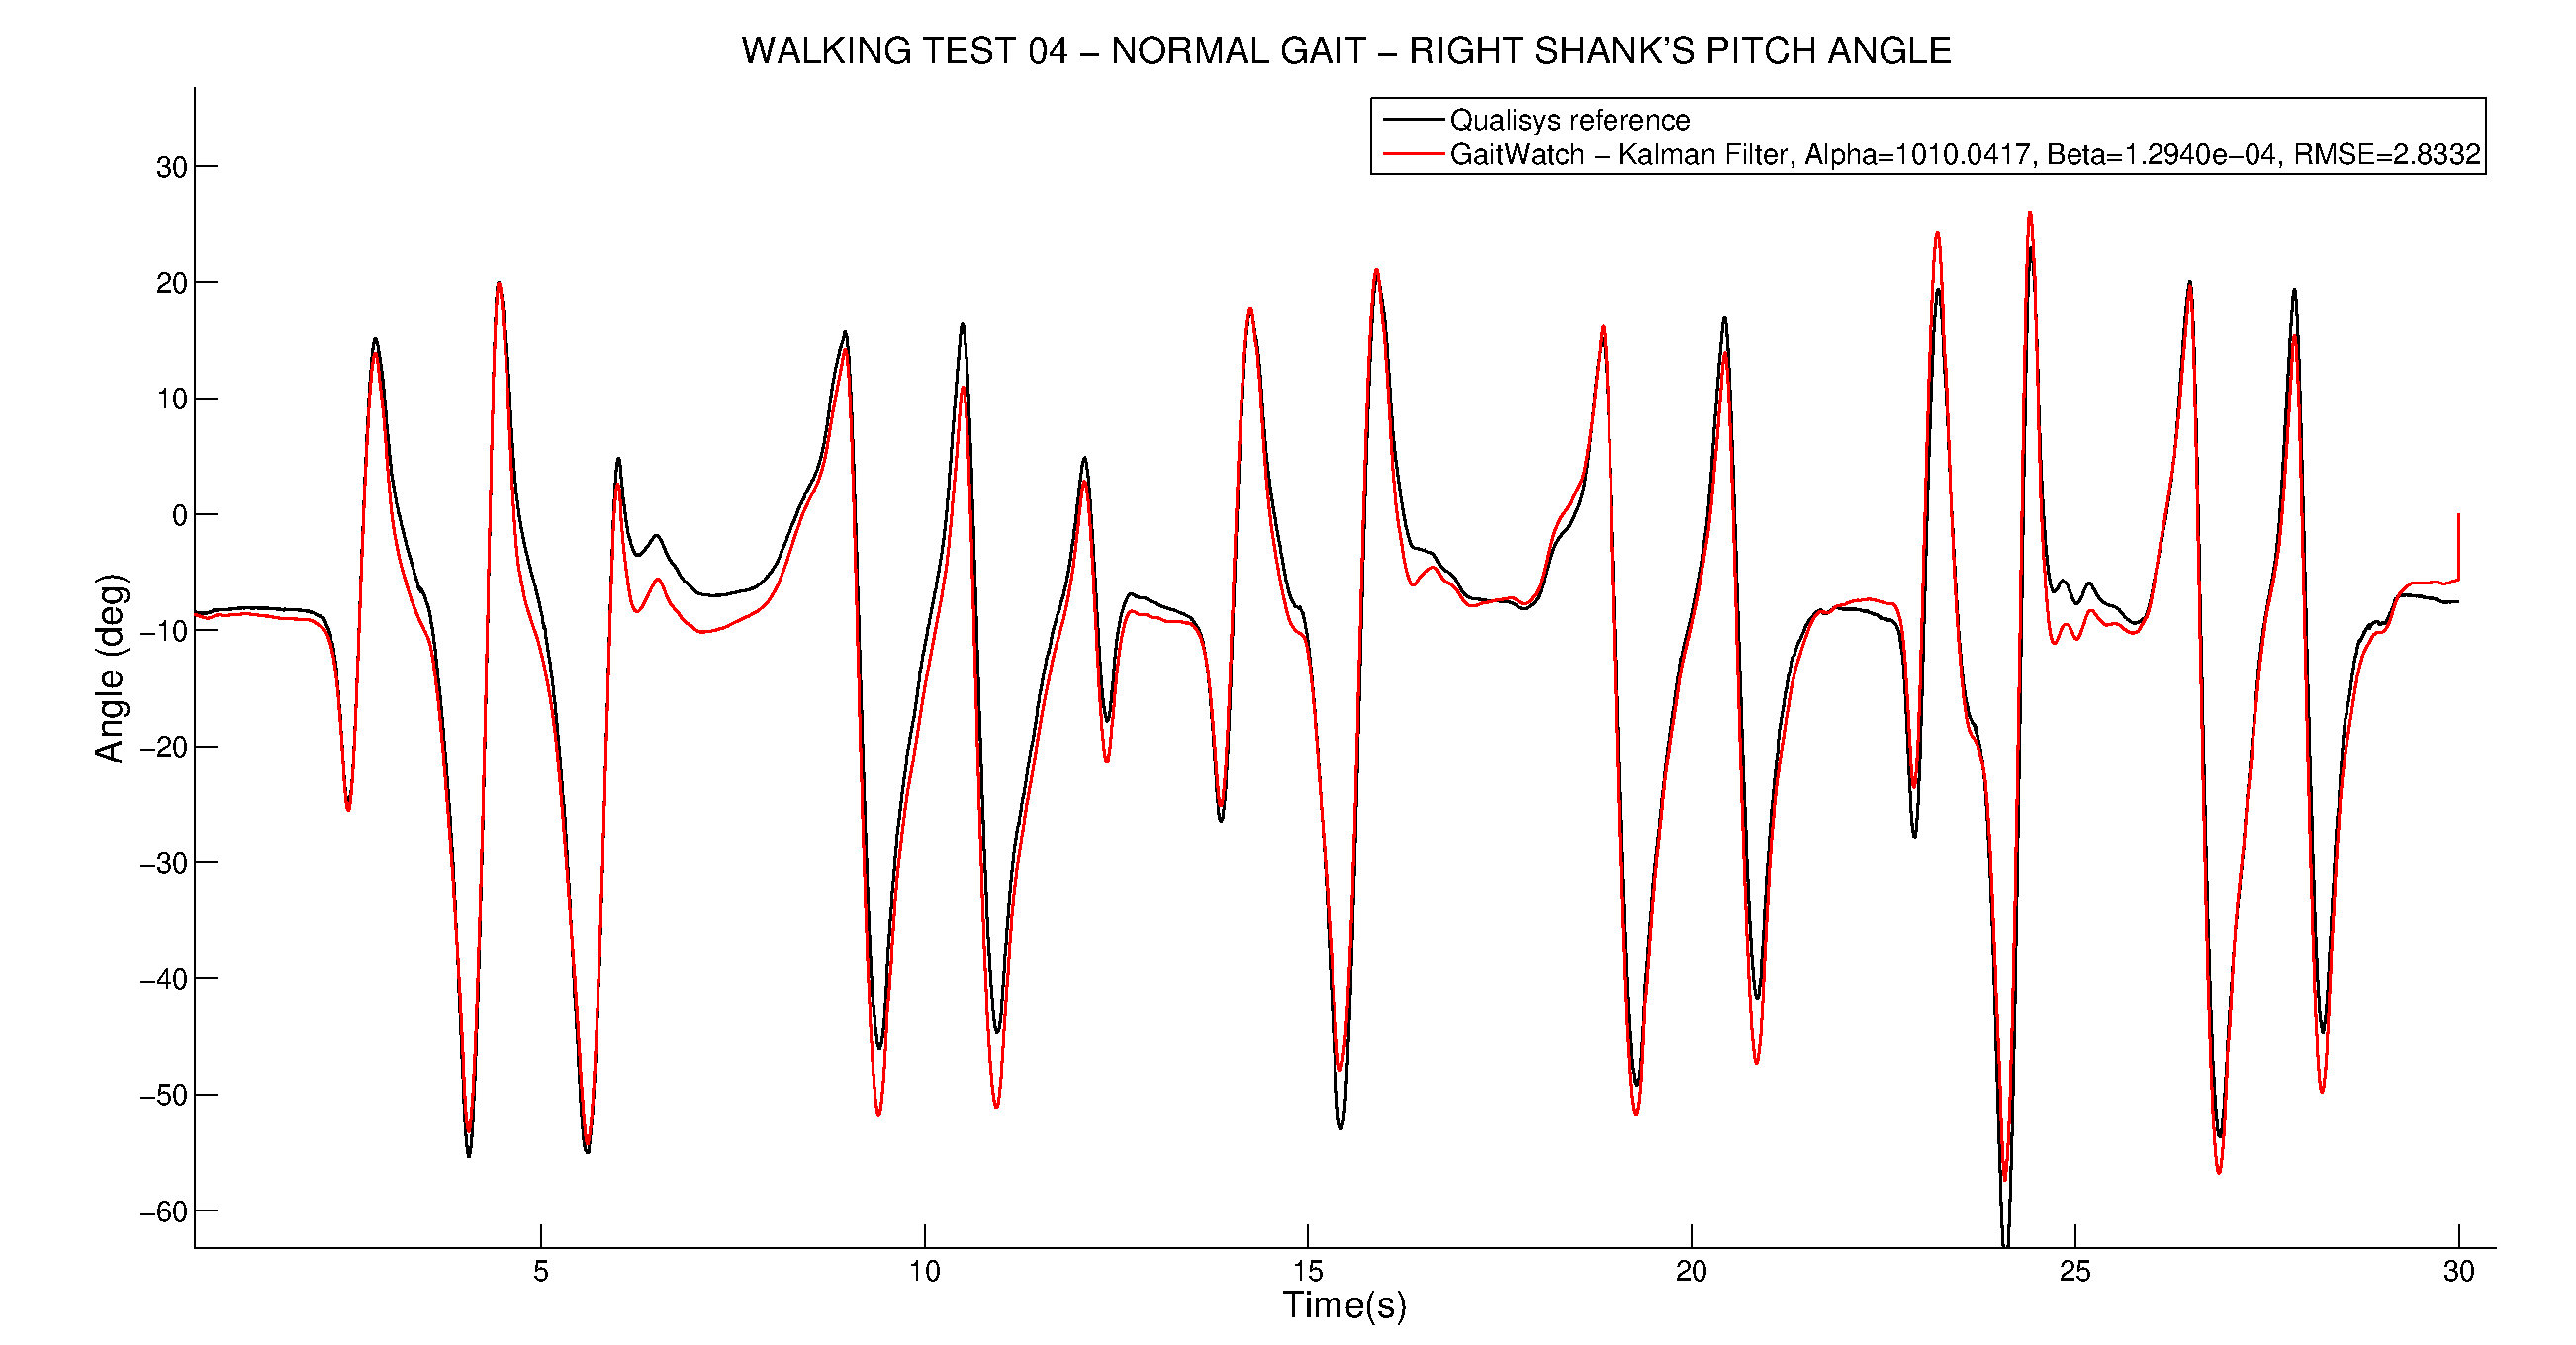
\includegraphics[width=1\textwidth]{figures/Walking_04_right_shank.eps}
\caption{Right shank's pitch angle during normal gait. (GaitWatch vs. Qualisys).}
\label{fig:Walking_04_right_shank}
\end{figure}

\begin{figure}[H]
\centering
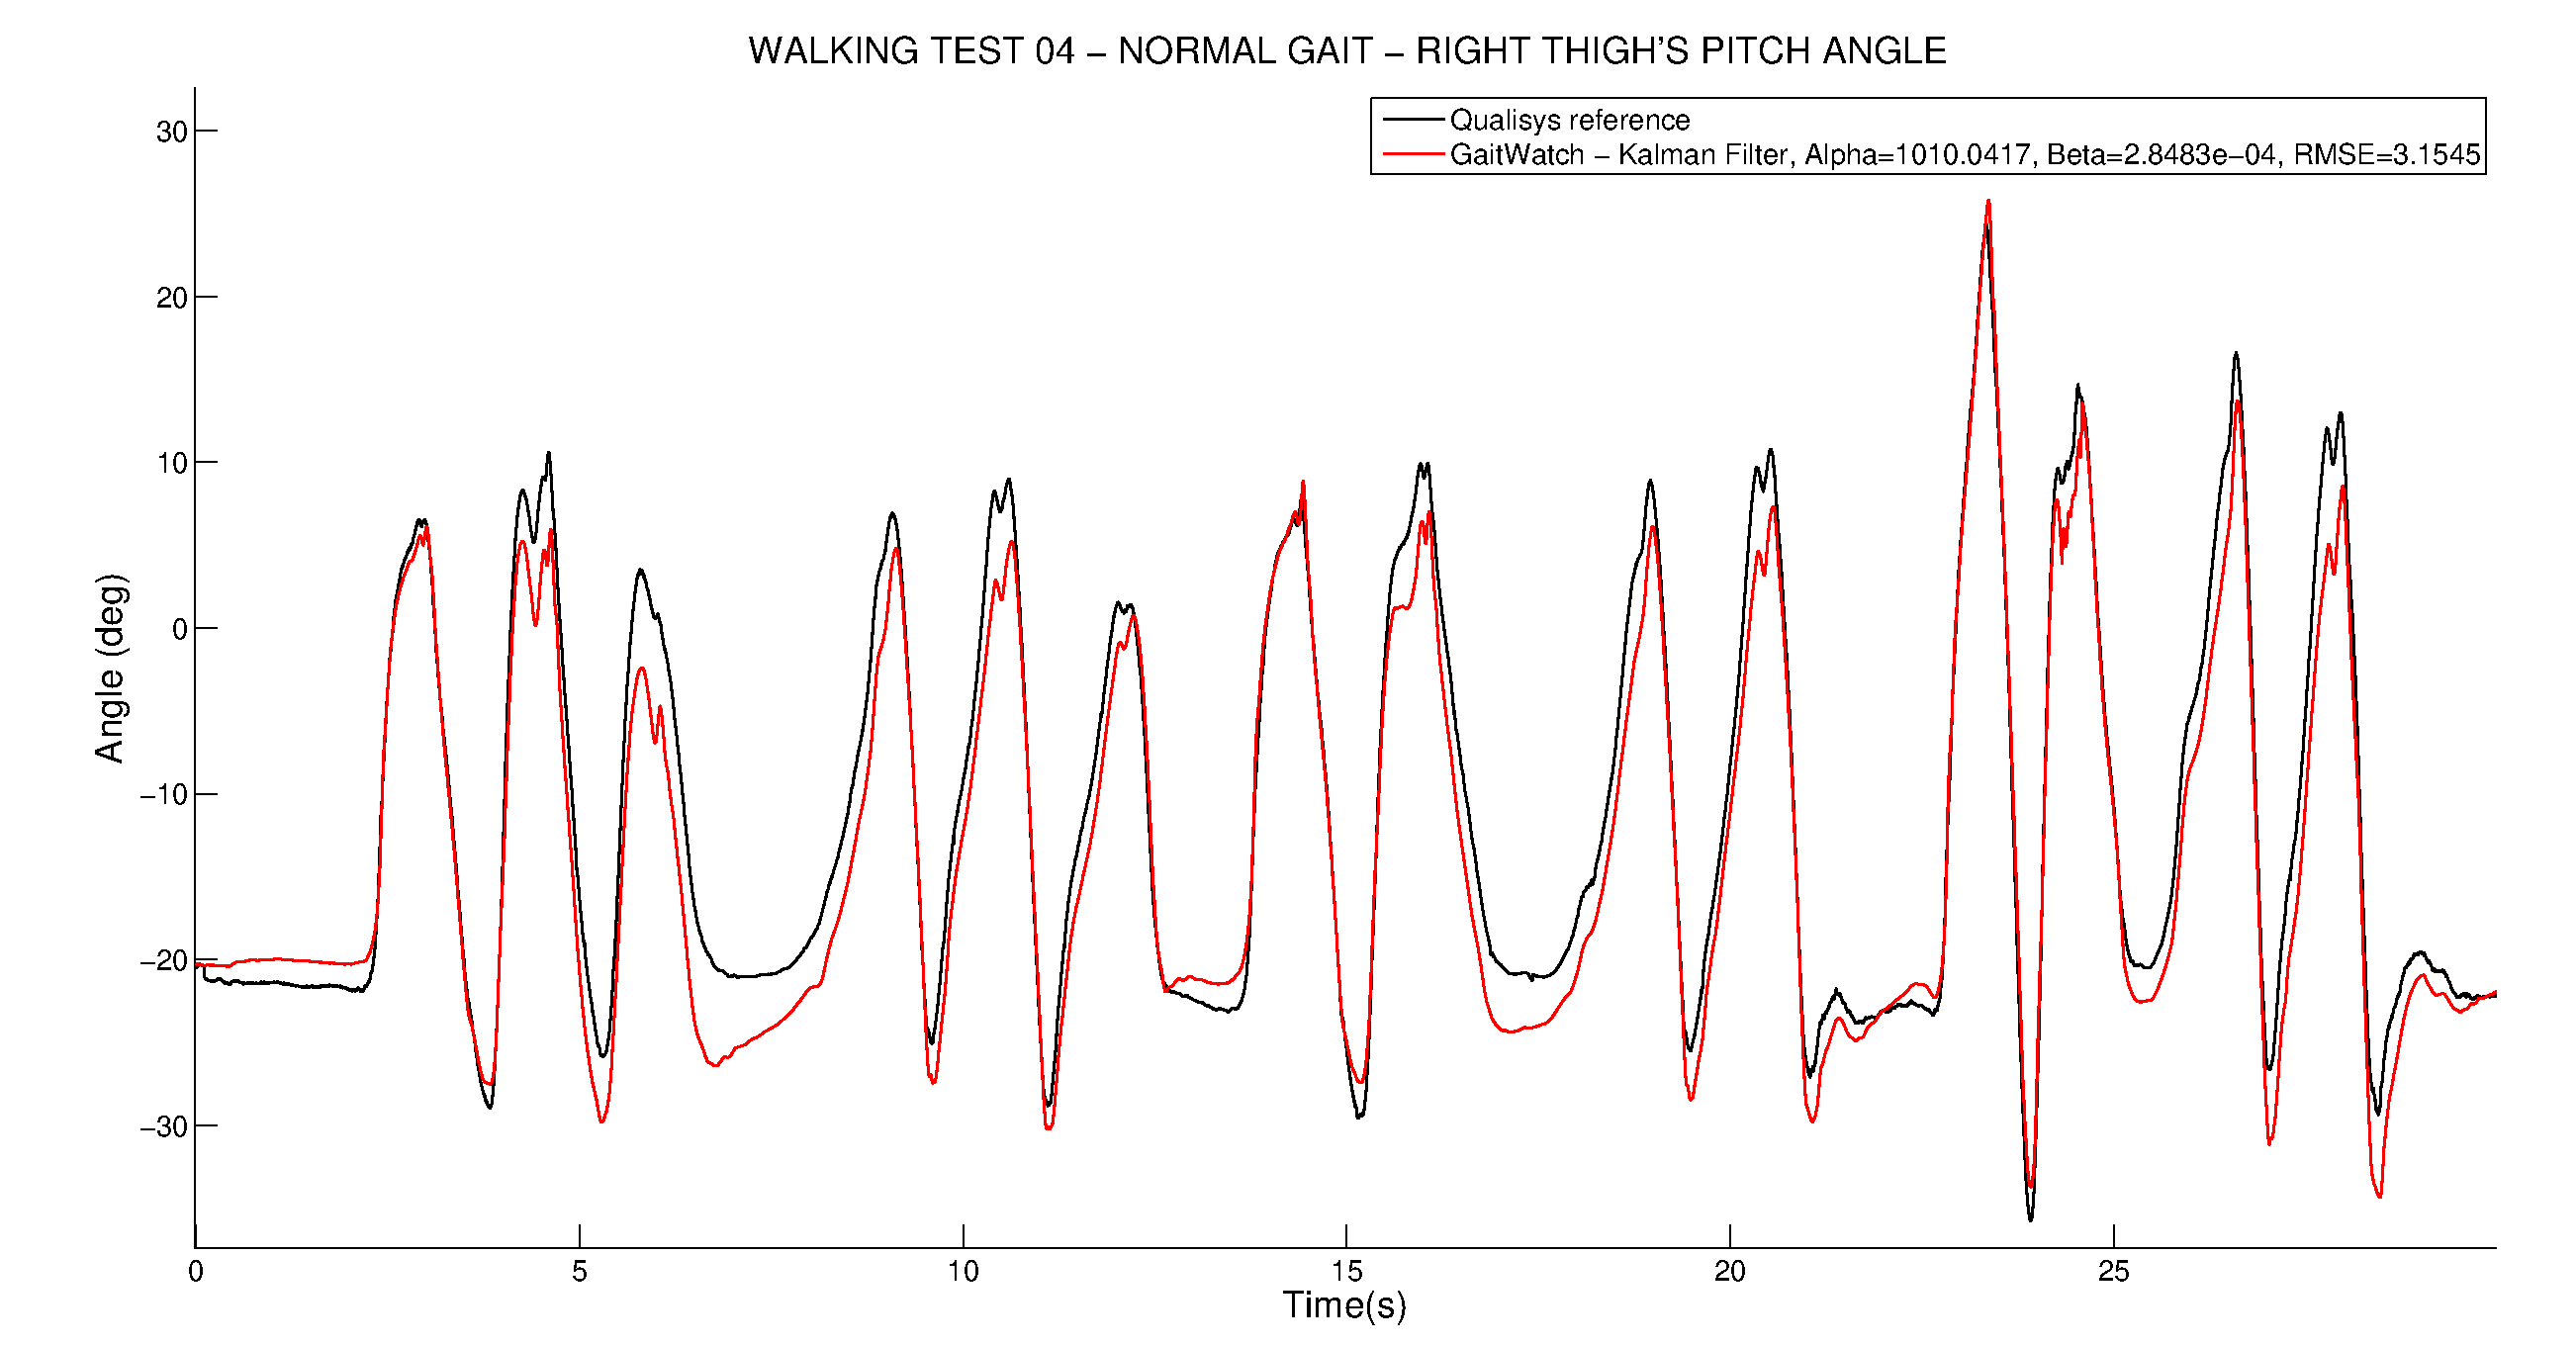
\includegraphics[width=1\textwidth]{figures/Walking_04_right_thigh.eps}
\caption{Right thigh's pitch angle during normal gait. (GaitWatch vs. Qualisys).}
\label{fig:Walking_04_right_thigh}
\end{figure}


  %\include{introduction}

  %\appendix
  %\include{HWappendix}
  %\include{FWappendix}
  %\include{phoneGatherAppendix}

  % Bibliografia
  %\renewcommand{\bibname}{Bibliograf�a}		% Nombre de la bibliograf�a
  %\clearemptydoublepage
  %\phantomsection
  \addcontentsline{toc}{chapter}{\numberline{}\bibname}% La a�ade al �ndice
  \bibliographystyle{unsrt}
  \sloppy
  \bibliography{references}
  
	\clearemptydoublepage

	

\end{document}
